% TO DO ANALISI DATI:
% 
% 1. Tutte le tabelle di verità e i grafici logici di timing:
%   - Porta AND *
%   - J/K *
%   - R/S *
%   - Clear
%   - Altri circuiti logici dell'ADC: registro di scorrimento, porte AND di pilotaggio dei J/K etc... per il paragrafo IV.
%
% 2. Immagini oscilloscopio dei segnale di clock e di clear
%   
%
% 3. Le tabelle con tutti i plot della calibrazione ADC
%
% 4. Le tabelle con tutti i plot di Nyquist (interpolati
%    con sinusoidi) dai dati di Arduino
%
% 5. Istogrammi code density
%
%

\documentclass[journal]{IEEEtran}

%%%%%%%%%%%%%%%%%%%%%%%%%%%%%%%%%%%%%%%%%%%%%%%%%%%%%%%%%%%%%%

\usepackage[italian]{babel}

% *** CITATION PACKAGES ***
\usepackage[style=ieee]{biblatex} 
\bibliography{digital.bib}    %your file created using JabRef
\usepackage{hyperref}

% *** MATH PACKAGES ***
\usepackage{amsmath}
 \usepackage{multirow}

% *** PDF, URL AND HYPERLINK PACKAGES ***
\usepackage{url}
% correct bad hyphenation here
\hyphenation{op-tical net-works semi-conduc-tor}
\usepackage{graphicx}  %needed to include png, eps figures
\usepackage{float}  % used to fix location of images i.e.\begin{figure}[H]

\usepackage{csquotes} % correzione errore compilazione

%%%%%%%%%%%%%%%%%%%%%%%%%%%%%%%%%%%%%%%%%%%%%%%%%%%%%%%%%%%%%


\begin{document}

% paper title
\title{Laboratorio di elettronica digitale\\ 
%\small{1 gennaio 2020}
}

% author names 
\author{\begin{center}Matteo Barbagiovanni\textsuperscript{1},
        Stefano Barbero\textsuperscript{2},
        Federico Malnati\textsuperscript{3},
        Valerio Pagliarino\textsuperscript{4},
        {\small \\
        \textsuperscript{1}
        matteo.barbagiovanni@edu.unito.it -
        \textsuperscript{2}
        stefano.barbero376@edu.unito.it
        \textsuperscript{3}
        federico.malnati@edu.unito.it -
        \textsuperscript{4}
        valerio.pagliarino@edu.unito.it}
        \end{center}}% <-this % stops a space
        
% The report headers
\markboth{Università degli Studi di Torino - C.d.L. Triennale in Fisica - 10/11/21 - A.A. 2021-2022    \quad   \quad \quad \quad   \quad \quad \quad  \quad   \quad \quad \quad   \quad \quad LABORATORIO DI ELETTRONICA \quad \quad }%do not delete next lines
{Shell \MakeLowercase{\textit{et al.}}: Bare Demo of IEEEtran.cls for IEEE Journals}

% make the title area
\maketitle


%%%%%%%%%%%%%%%%%%%%%%%%%%%%%%%%%%%%%%%%%%%%%%%%%%%%%%%%%%%%%
%% Introduzione 
%%%%%%%%%%%%%%%%%%%%%%%%%%%%%%%%%%%%%%%%%%%%%%%%%%%%%%%%%%%%%

\begin{abstract} 
Dopo aver analizzato i principali circuiti analogici che consentono l'amplificazione e il condizionamento dei segnali, in questa seconda relazione di laboratorio si studieranno alcune tecniche di elettronica digitale con l'obiettivo di realizzare un convertitore ADC (Analog to Digital Converter) ad approssimazioni successive, analizzando la catena del segnale dall'ingresso analogico fino alla memorizzazione dei dati su scheda di memoria. Inizialmente, dopo aver introdotto la famiglia di integrati digitali 7400 che verrà utilizzata, verranno prese in esame alcune funzioni logiche fondamentali come le porte AND, NAND, NOT, i flip-flop di tipo set-reset e J-K di cui verranno studiate le tabelle di verità e talvolta le funzioni di trasferimento. A questo punto verrà introdotta l'architettura generale del convertitore SAR, seguita da una rapida caratterizzazione dei sottocircuiti che lo compongono: il registro a scorrimento con la relativa logica di controllo, i J-K, il DAC e lo stadio analogico. Successivamente, dopo aver assemblato il circuito, si passerà alla verifica di alcune caratteristiche quantitative di base, con la calibrazione del DAC e dell'ADC al completo.
A questo punto si potranno finalmente eseguire le prime operazioni di campionamento con l'ausilio dell'oscilloscopio: dapprima di segnali costanti e poi di forme d'onda variabili nel tempo. Infine, verrà installato un circuito analogico di \textit{sample holding} per migliorare le prestazioni del dispositivo nel campionamento di segnali variabili e si prevederà un sistema di registrazione delle misure mediante una scheda a microcontrollore. Quest'ultimo passaggio renderà possibile la verifica del teorema del campionamento di Nyquist-Shannon e la valutazione della linearità del dispositivo realizzato con il metodo della \textit{code density}. 
\end{abstract}

%%%%%%%%%%%%%%%%%%%%%%%%%%%%%%%%%%%%%%%%%%%%%%%%%%%%%%%%%%%%%
%%%%%%%%%%%%%%%%%%%%%%%%%%%%%%%%%%%%%%%%%%%%%%%%%%%%%%%%%%%%%

\section{Componenti utilizzati}

In aggiunta alla strumentazione da laboratorio già descritta nella precedente relazione e all'OPA LM741, per la realizzazione delle esperienze di elettronica digitale sono stati utilizzati i componenti descritti brevemente nei sotto-paragrafi seguenti.


\subsection{Logica TTL serie 7400}
I ciruiti logici descritti nella presente relazione di laboratorio sono stati realizzati utilizzando la famiglia di integrati 7400 che utilizza lo standard TTL. Questi componenti sono realizzati mediante transistor bipolari e resistori su die a basso livello di integrazione e riconoscono come segnale di livello alto una tensione da 2 V a 5 V e come segnale di livello basso una tensione da a 0 V a 0.8 V; lo standard prevede un margine di rumore pari a 0.4 V. In laboratorio sono stati utilizzati:
\begin{itemize}
    \item \textbf{SN74LS164M} - Un registro a scorrimento con capacità di memoria di 8 bit che supporta frequenze di clock fino a 25 MHz con un assorbimento di corrente inferiore a 54 mA dotato di due ingressi seriali in NAND tra loro e un ingresso di clear asincrono. 
    
   \cite{D}
    
    \item \textbf{74LS76AN} - Un integrato contenente due flip-flop di tipo J-K che lavorano sul fronte di discesa del clock (\textit{negative-edge triggered}) con ingressi separati per il clock e per il segnale di clear asincrono. Il componente supporta frequenze di commutazione fino a 30 MHz e ritardo di propagazione dei segnali di clock, clear e PRE inferiore a 25 ns. Dal momento che le uscite Q di questi J-K verranno utilizzate per alimentare una rete di resistenze per realizzare un DAC R-2R, è interessante riportare che questi componenti supportano correnti di corto-circuito sulle uscite fino a 100 mA in regime impulsato.
    \cite{E}
    
    \item \textbf{SN74LS08N} - Un integrato che implementa 4 porte AND in logica positiva mediante uno stadio di ingresso realizzato con transistor BJT multi-emettitore e uscita totem-pole. Questo componente ha tempi di commutazione  di 17.5 ns per portarsi allo stato basso e 12 ns per portarsi allo stato alto.
    \cite{F}
    
    \item \textbf{SN74LS00N} - Un integrato che implementa 4 porte NAND in logica positiva con tempi di commutazione di 9 ns e 10 ns rispettivamente per portarsi allo stato basso o allo stato alto.
    \cite{G}
    
    \item \textbf{SN74LS04} - Un integrato che implementa 6 porte NOT (inverter) con tempi di commutzione di 12 ns e 8 ns rispettivamente per portarsi allo stato basso e allo stato alto.
    \cite{H}
    
\end{itemize}

\begin{figure}[H]%[!ht]
\begin{center}
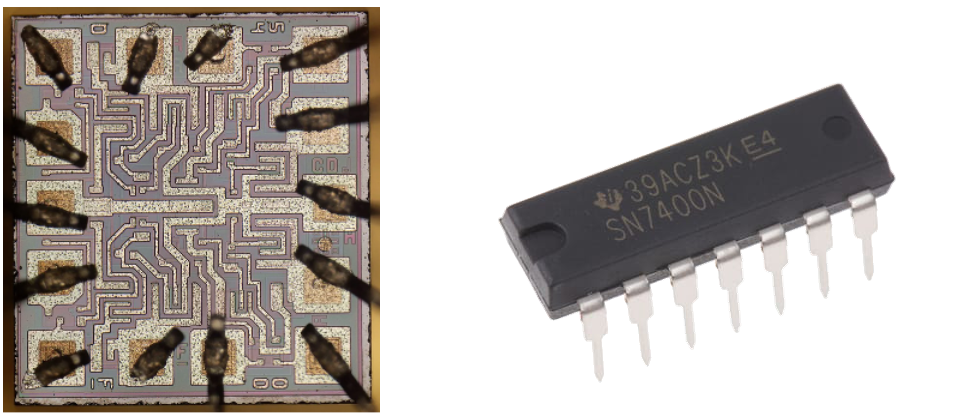
\includegraphics[width=0.40\textwidth]{lab-reports/Schematics-and-graphics/SN7400N.png}
\caption{Fotografia del DIE e del \textit{package} plastico DIP \textit{(Dual Inline Package)} dell'integrato con 2 porte NAND SN7400N}
\label{fig:integrated_nand}
\end{center}
\end{figure}

\subsection{Transistor di interfaccia PN2222A}
Gli integrati logici appena descritti, appartenendo alla famiglia TTL con stato alto a 5V, non possono essere collegati direttamente all'uscita degli amplificatori operazionali presenti nello stadio analogico del SAR, che operano tra +15V e -15V, si rende quindi necessaria l'introduzione di un transistor di interfaccia come il PN2222A, un BJT NPN \textit{general purpose} con $h_{fe}$ compreso tra 100 e 300 che tollera correnti di collettore fino a 600 mA. Questo dispositivo verrà utilizzato in configurazione ad emettitore comune in modalità interdizione / saturazione.
\cite{I}


\subsection{Integrato di \textit{sample holding} LF398}
Il convertitore SAR tratttato in questa relazione può campionare segnali variabili nel tempo sotto l'ipotesi di piccole variazioni di questi durante ciascun ciclo di campionamento e questo implica di utilizzare una frequenza di campionamento molto maggiore della frequenza delle armoniche di Fourier del segnale in ingresso. Per ottenere prestazioni migliori, raggiungendo il limite posto dal teorema di campionamento di Nyquist-Shannon, è necessario introdurre un circuito in grado di mantenere costante la tensione all'ingresso dell'ADC fino a quanto il ciclo di conversione non viene completato. Questo viene realizzato mediante l'integrato monolitico \textit{sample and hold} LF398, che prevede un ingresso compatibile con la logica TTL per controllare la finestra di campionamento, due pin per il collegamento del condensatore che permetterà il mantenimento della tensione in uscita, due pin di alimentazione duale $\pm$ 15V e naturalmente i pin di ingresso e di uscita del segnale analogico. L'integrato necessita di meno di 10 $\mu s$ per effettuare il campionamento e il datasheet riporta una stabilità del guadagno pari allo 0.002 \%.
\cite{J}

\subsection{Scheda a microcontrollore}
Nell'ultima fase dell'esperienza di laboratorio verrà realizzato un semplice sistema di registrazione dei valori acquisiti utilizzando un microcontrollore \textit{Atmel ATmega328P} basato sull'architettura Harvard RISC a 8 bit interfacciato con un lettore di schede microSD. Questo MCU viene impiegato con un oscillatore esterno al quarzo a 16 MHz per il clock, dispone di 32 KB di memoria ISP flash e nel nostro caso è installato su una scheda Arduino che ospita anche un secondo microcontrollore \textit{Atmel ATmega16u2} con funzione di interfaccia di programmazione USB. La funzione di questo dispositivo è quella di leggere lo stato delle uscite dei J-K, corrispondente alla rappresentazione binaria del segnale campionato, e di scrivere su un file salvato una scheda microSD a cui è connesso mediante una linea seriale SPI.

%%%%%%%%%%%%%%%%%%%%%%%%%%%%%%%%%%%%%%%%%%%%%%%%%%%%%%%%

\section{Caratterizzazione dei circuiti logici fondamentali}

\subsection{Verifica della tabella di verità della porta AND}
Una porta AND è un gate logico digitale con due o più ingressi e un'uscita che esegue la congiunzione logica. L'output di tale componente rispetta la seguente tabella di verità:
\begin{center}
\begin{tabular}{ |c|c|c| } 
 \hline
 A & B & OUT \\ \hline 
 0 & 0 & 0 \\ \hline
 1 & 0 & 0 \\ \hline
 0 & 0 & 0 \\ \hline
 1 & 1 & 1 \\ \hline
 
 \hline
\end{tabular}
\end{center}
In laboratorio utilizzando l'integrato \textbf{SN74LS08N} e fornendo in ingresso due onde quadre di frequenza 5 Hz oscillanti tra 0 e 5 V e sfasate di un quarto di periodo si è ottenuta la  \textit{figura \ref{fig:AND-table}} 
\begin{figure}[H]%[!ht]
\begin{center}
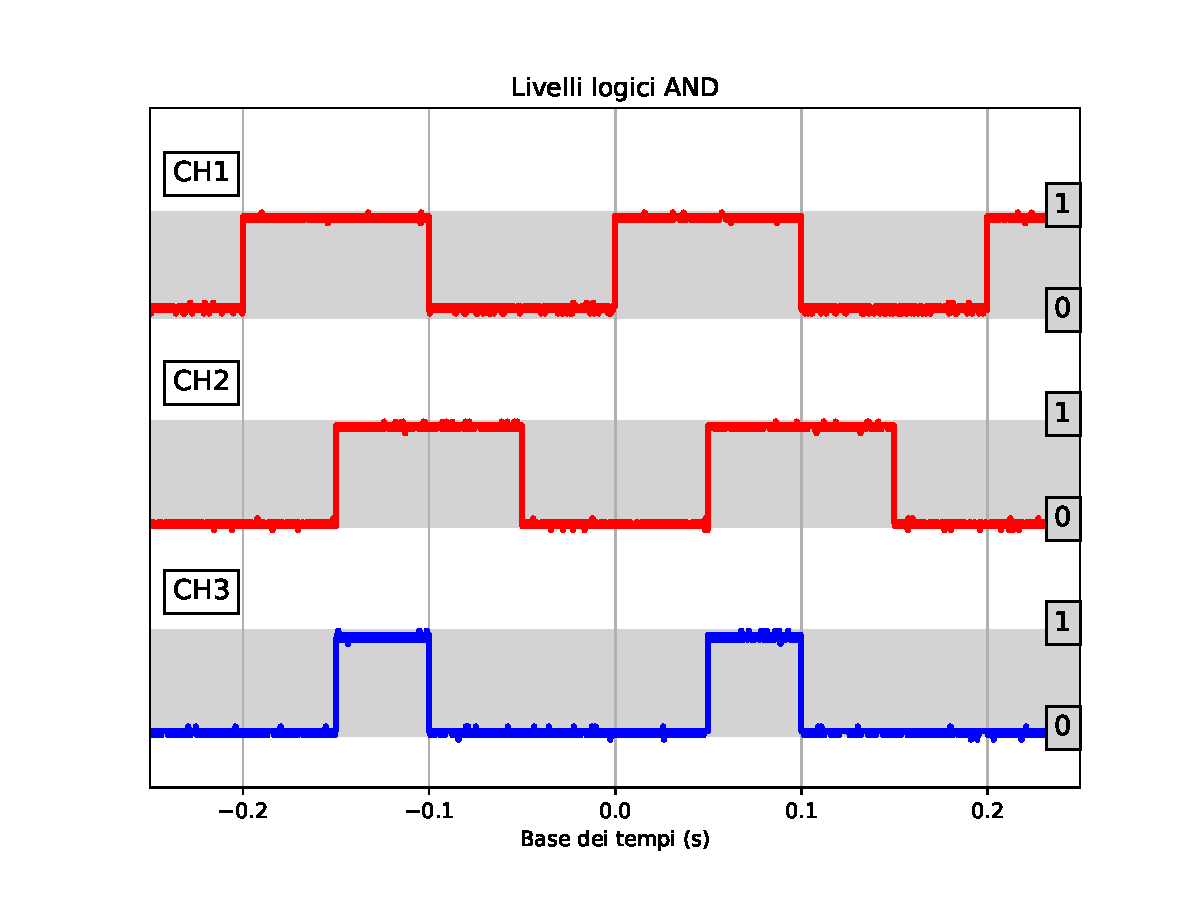
\includegraphics[width=0.40\textwidth]{analysis/output/AND-all.pdf}
\caption{Verifica della tabella di verità della porta logica AND}
\label{fig:AND-table}
\end{center}
\end{figure}

Dal grafico si evincono tutti i possibili scenari, notando in particolare che il  segnale in uscita risulta allo stato logico 1 solamente nel momento in cui entrambi gli ingressi sono in tale livello.


\subsection{Studio della caratteristica di trasferimento della porta NAND}
Testo

\begin{figure}[H]%[!ht]
\begin{center}
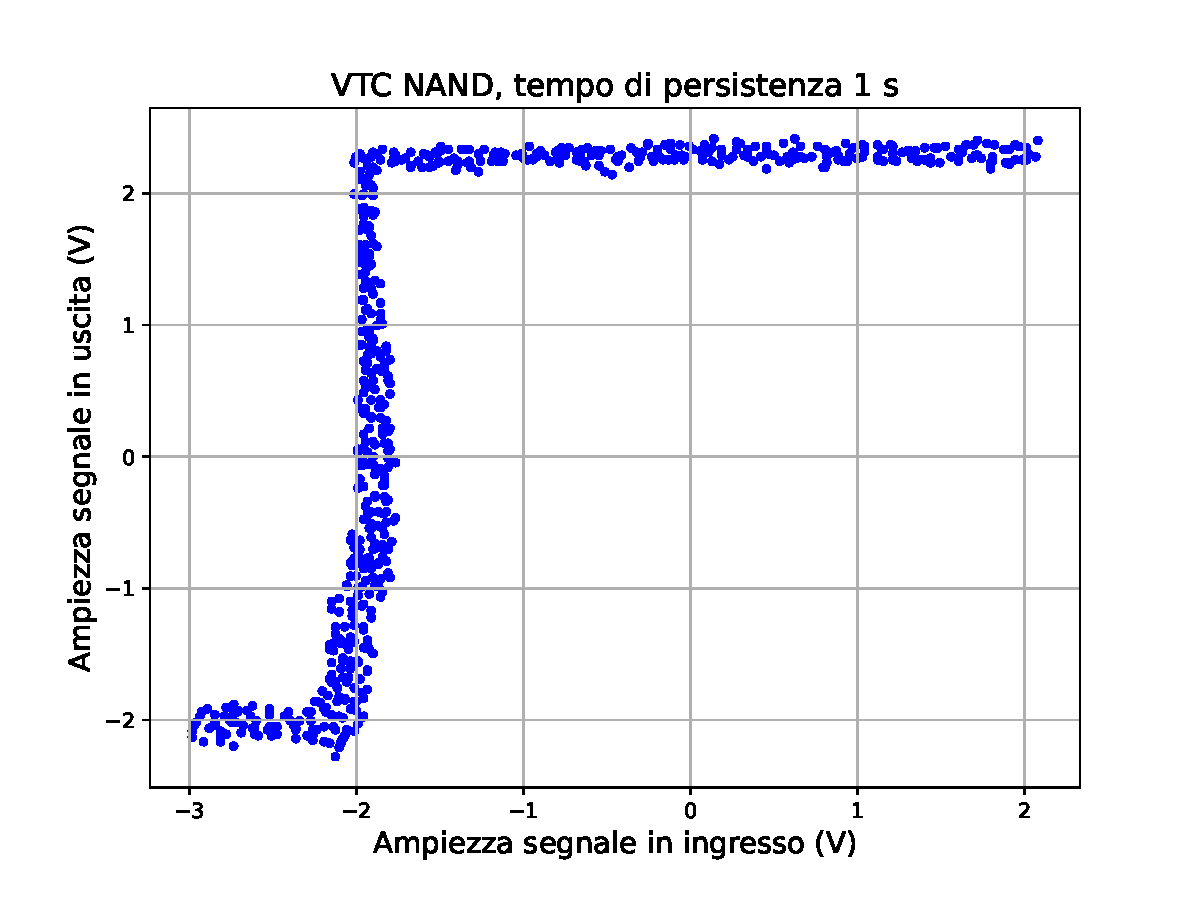
\includegraphics[width=0.40\textwidth]{analysis/output/NAND-XY.pdf}
\caption{Forma d'onda generata dall'anello di inverter}
\label{fig:graph_ring_oscillator}
\end{center}
\end{figure}


\subsection{Studio della caratteristica di trasferimento della porta NOT}
Testo

\begin{figure}[H]%[!ht]
\begin{center}
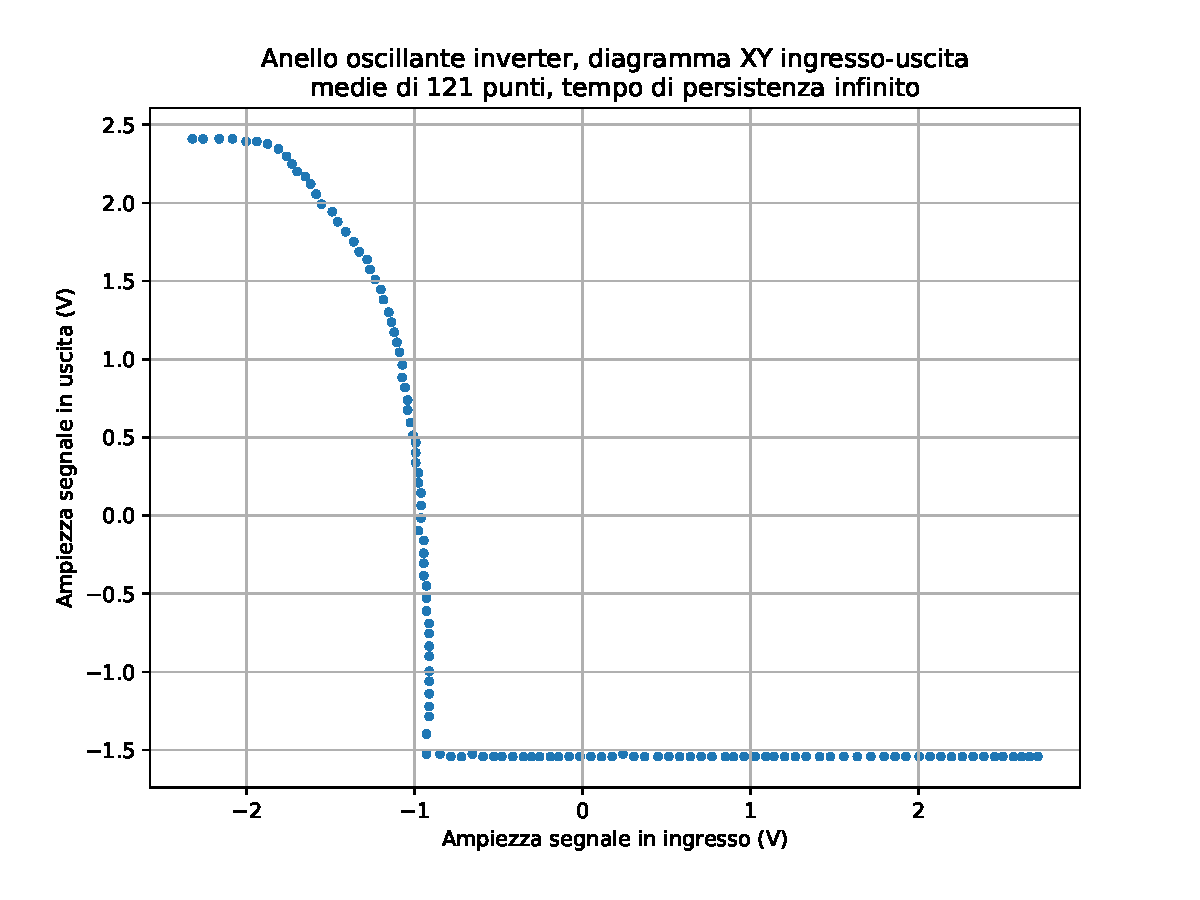
\includegraphics[width=0.45\textwidth]{analysis/output/inverter_ring_xy.pdf}
\caption{Caratteristica di trasferimento della porta NOT}
\label{fig:inverter_ring_xy}
\end{center}
\end{figure}


\subsection{Flip-flop di tipo set - reset}
Testo

\begin{figure}[H]%[!ht]
\begin{center}
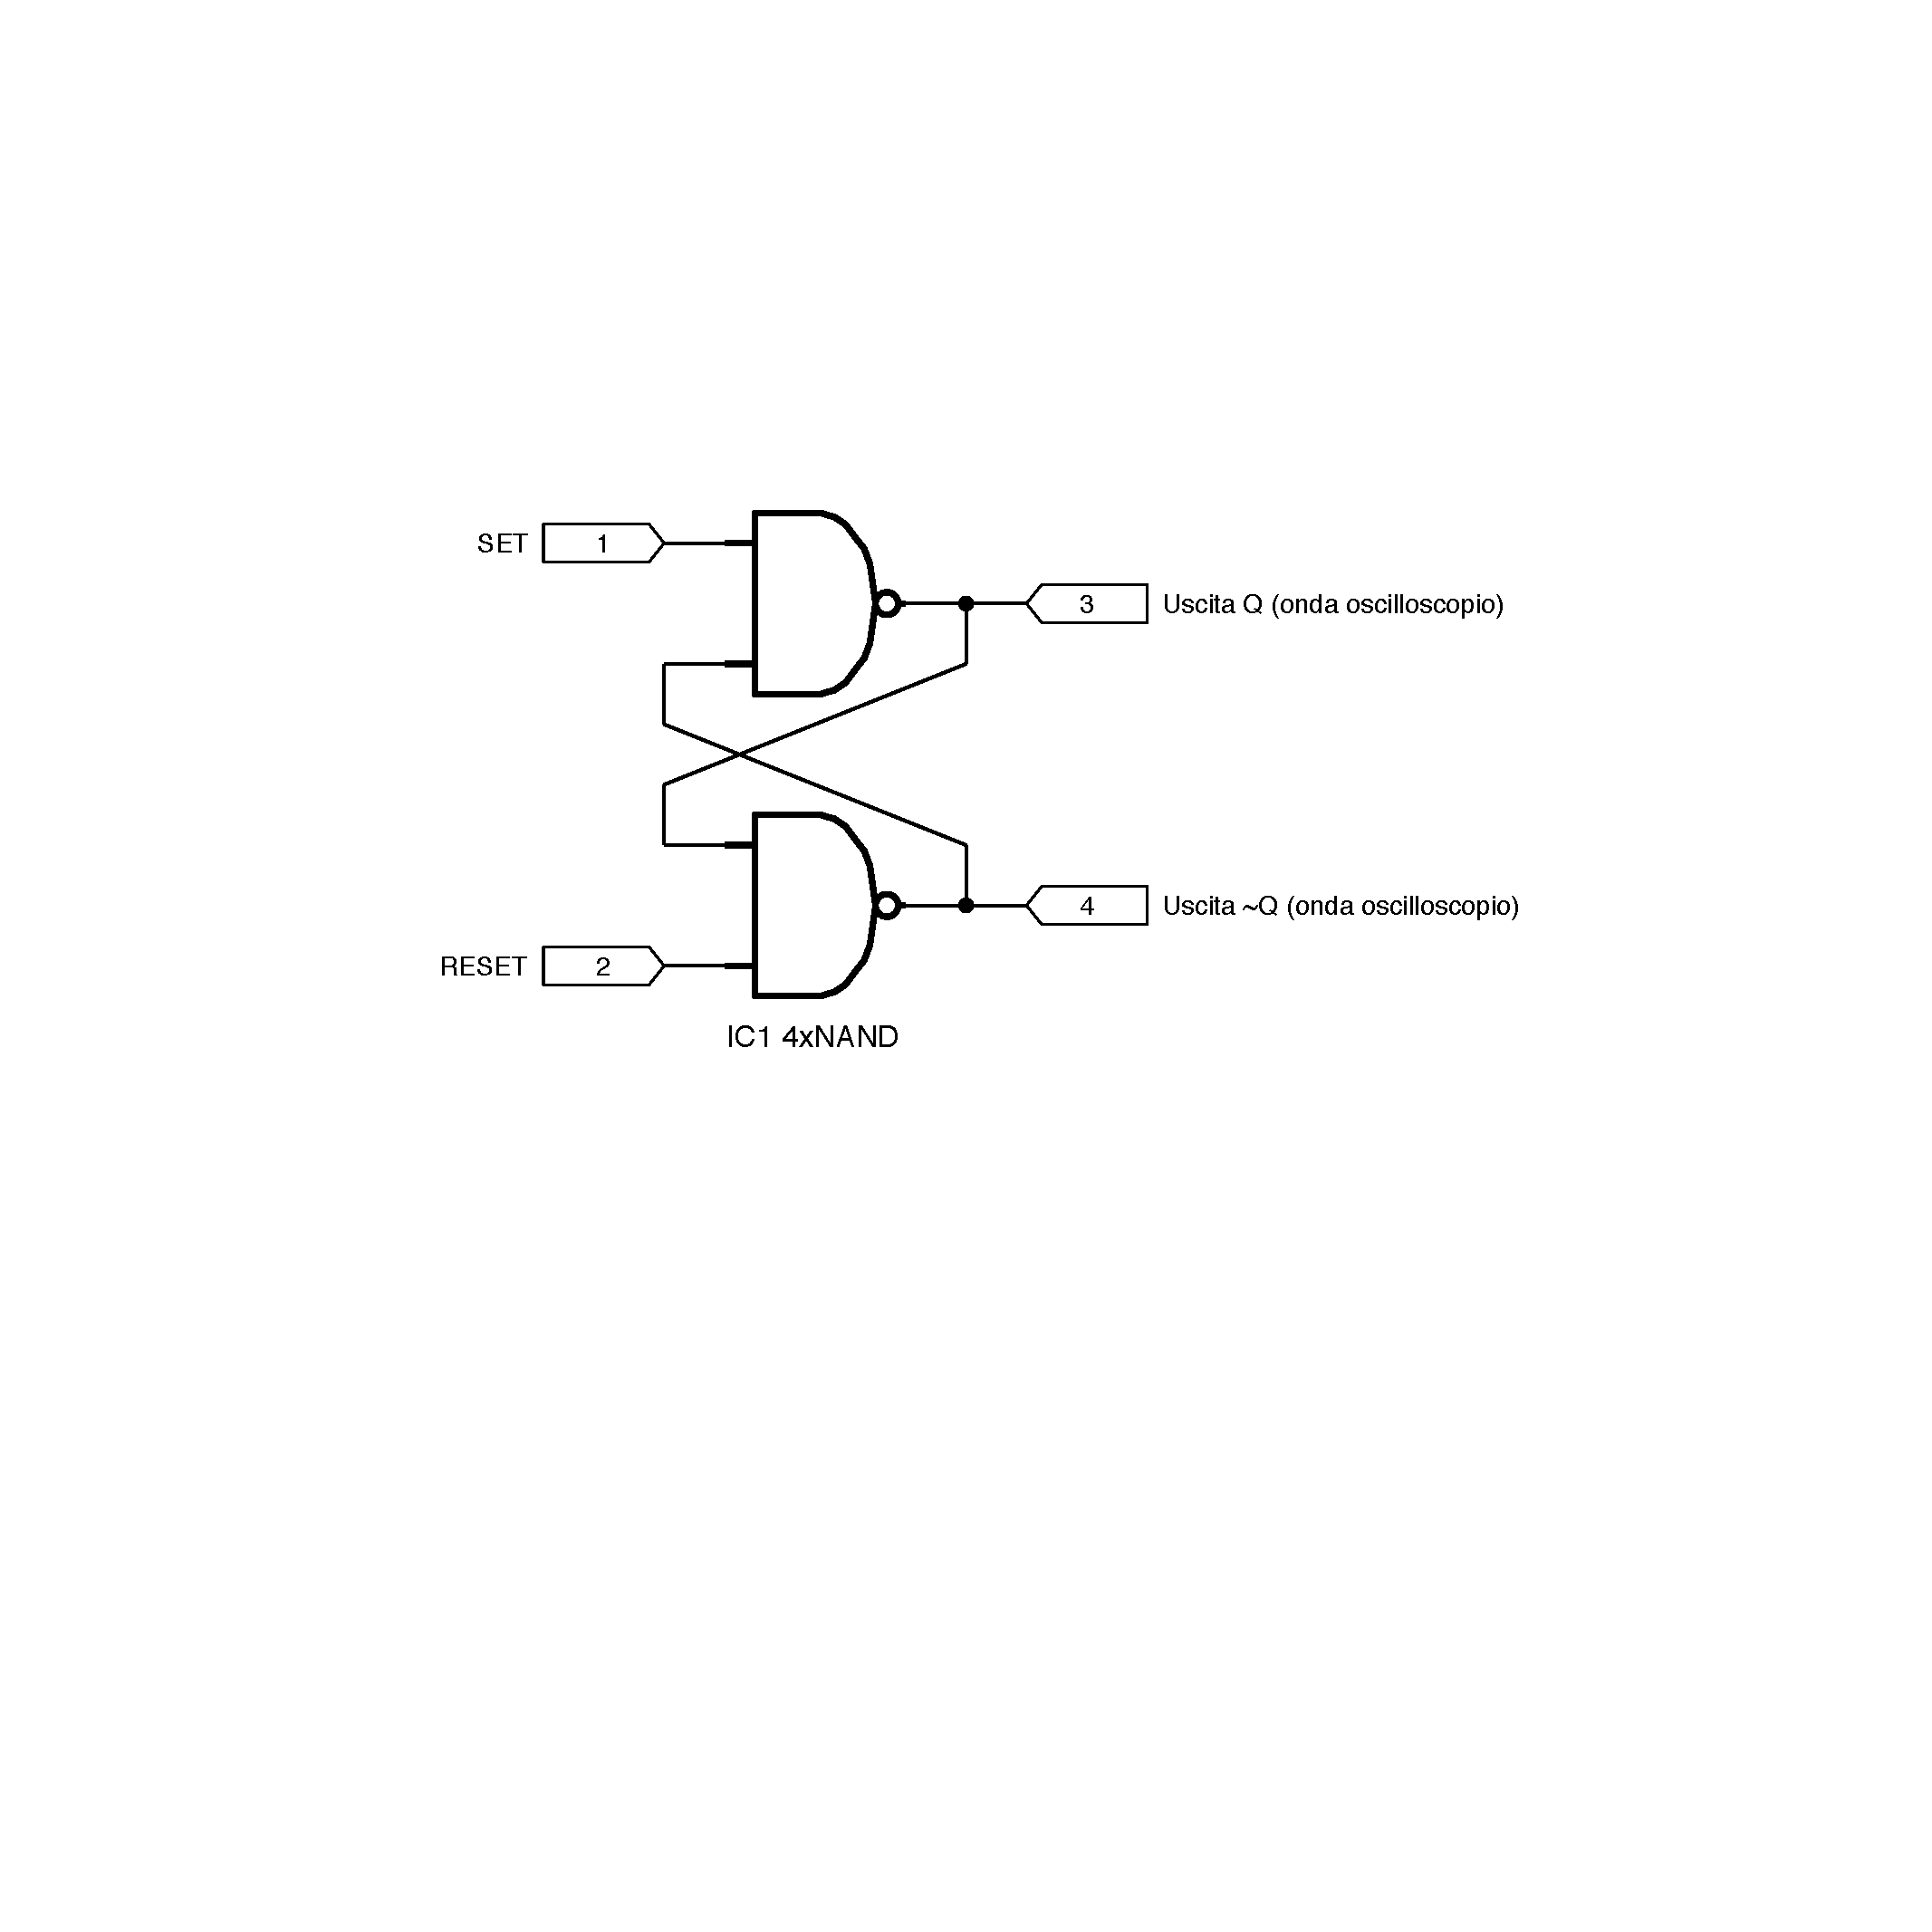
\includegraphics[width=0.30\textwidth]{sch-simulations/digital/output/flip-flop-RS.pdf}
\caption{Logica interna del flip-flop set-reset}
\label{fig:circuit_flip_flop}
\end{center}
\end{figure}
\begin{center}
\begin{tabular}{ |c|c|c|c| } 
 \hline
 S & R & Q & $\overline{Q}$ \\ \hline 
 0 & 0 & 1 & 1 \\ \hline
 0 & 1 & 1 & 0 \\ \hline
 1 & 0 & 0 & 1 \\ \hline
 1 & 1 & 0 & 1 \\ \hline
 1 & 1 & 1 & 0 \\ \hline
\end{tabular}
\end{center}
\begin{figure}[H]%[!ht]
\begin{center}
\includegraphics[width=0.40\textwidth]{analysis/output/set-reset-table.pdf}
\caption{Verifica della tabella di verità di un flip-flop di tipo set-reset realizzato con porte NAND}
\label{fig:graph_ring_oscillator}
\end{center}
\end{figure}



\subsection{Verifica della tabella di verità del flip-flop di tipo J-K}
Testo

\begin{figure}[H]%[t]
\centering
\begin{center}
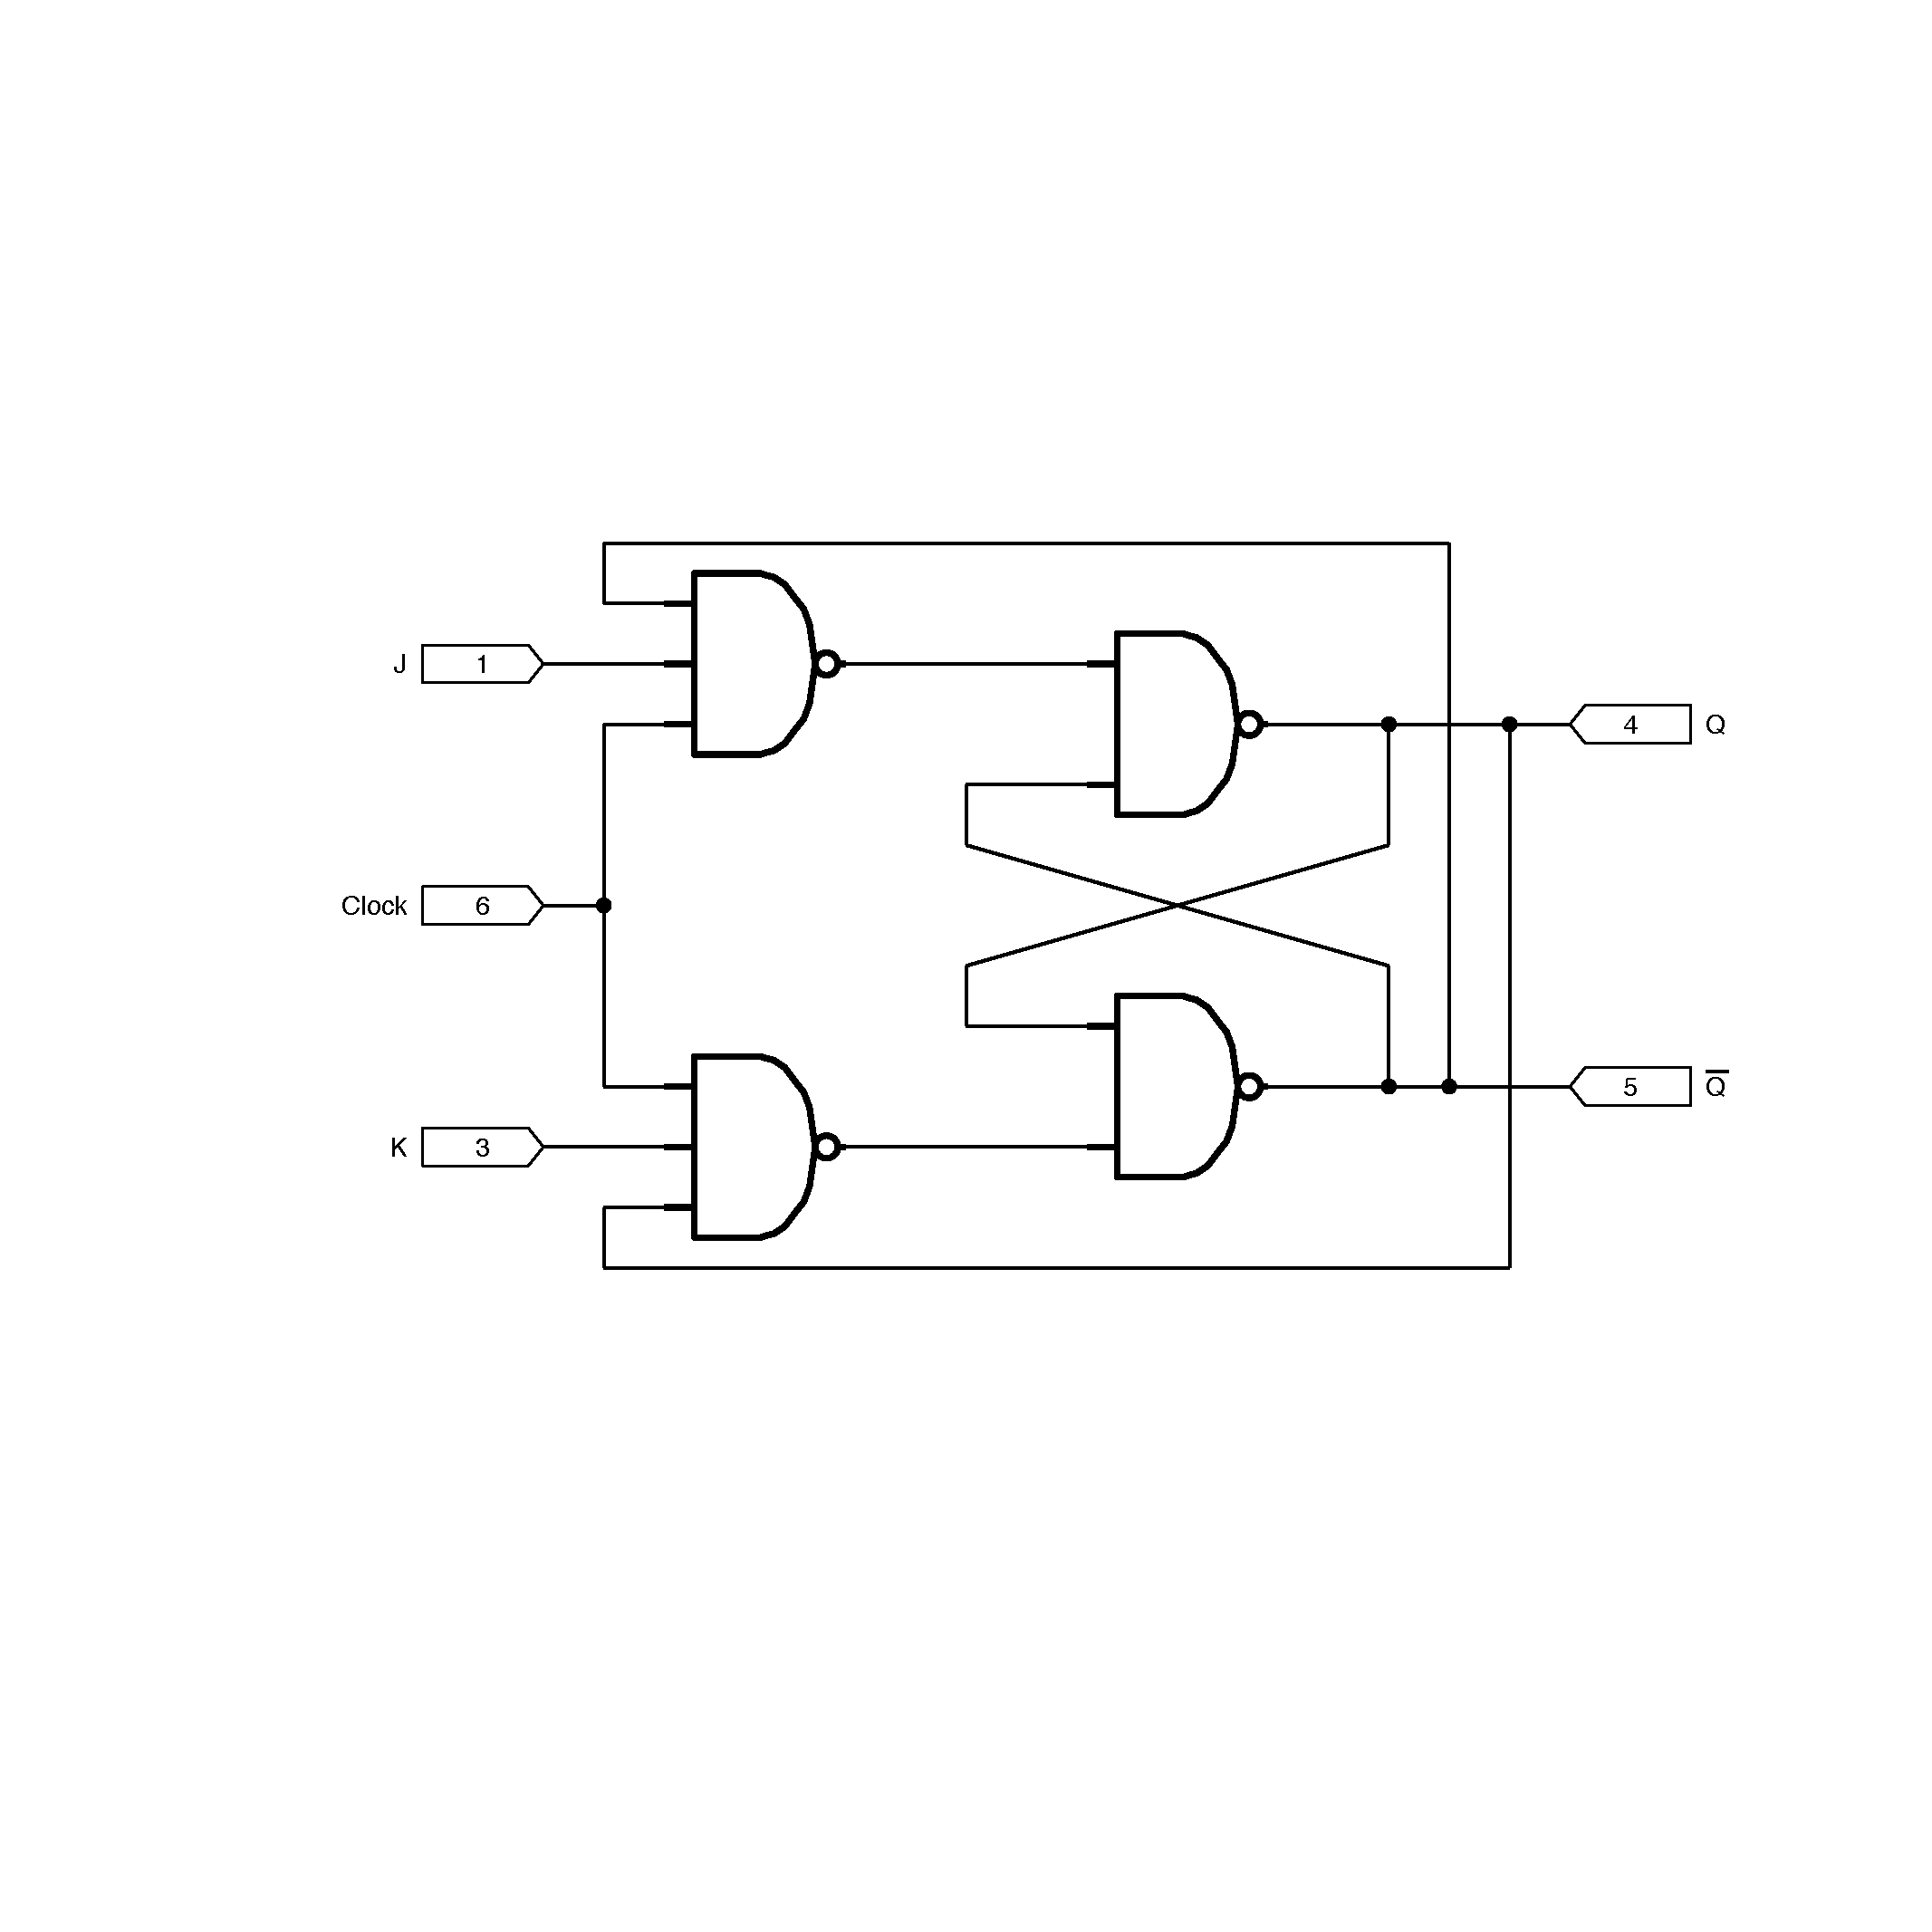
\includegraphics[width=0.40\textwidth]{sch-simulations/digital/output/flip-flop-JK.pdf}
\end{center}
\caption{Logica interna del flip-flop JK}
\label{fig:circuit_JK}
\end{figure}

\begin{center}
\begin{tabular}{ |c|c|c|c|c| } 
 \hline
 J & K & Q & $\overline{Q}$ & $ Q_{n + 1} $ \\ \hline 
 0 & 0 &  &  & $Q_n$ \\ \hline
 1 & 0 & 0 & 1 & 1 \\ \hline
 1 & 0 & 1 & 0 & 1\\ \hline
 0 & 1 & 0 & 1 & 0 \\ \hline
 0 & 1 & 1 & 0 & 0 \\ \hline
 1 & 1 &  & & $\overline{Q_n}$ \\ \hline
\end{tabular}
\end{center}

\begin{figure}[H]%[!ht]
\begin{center}
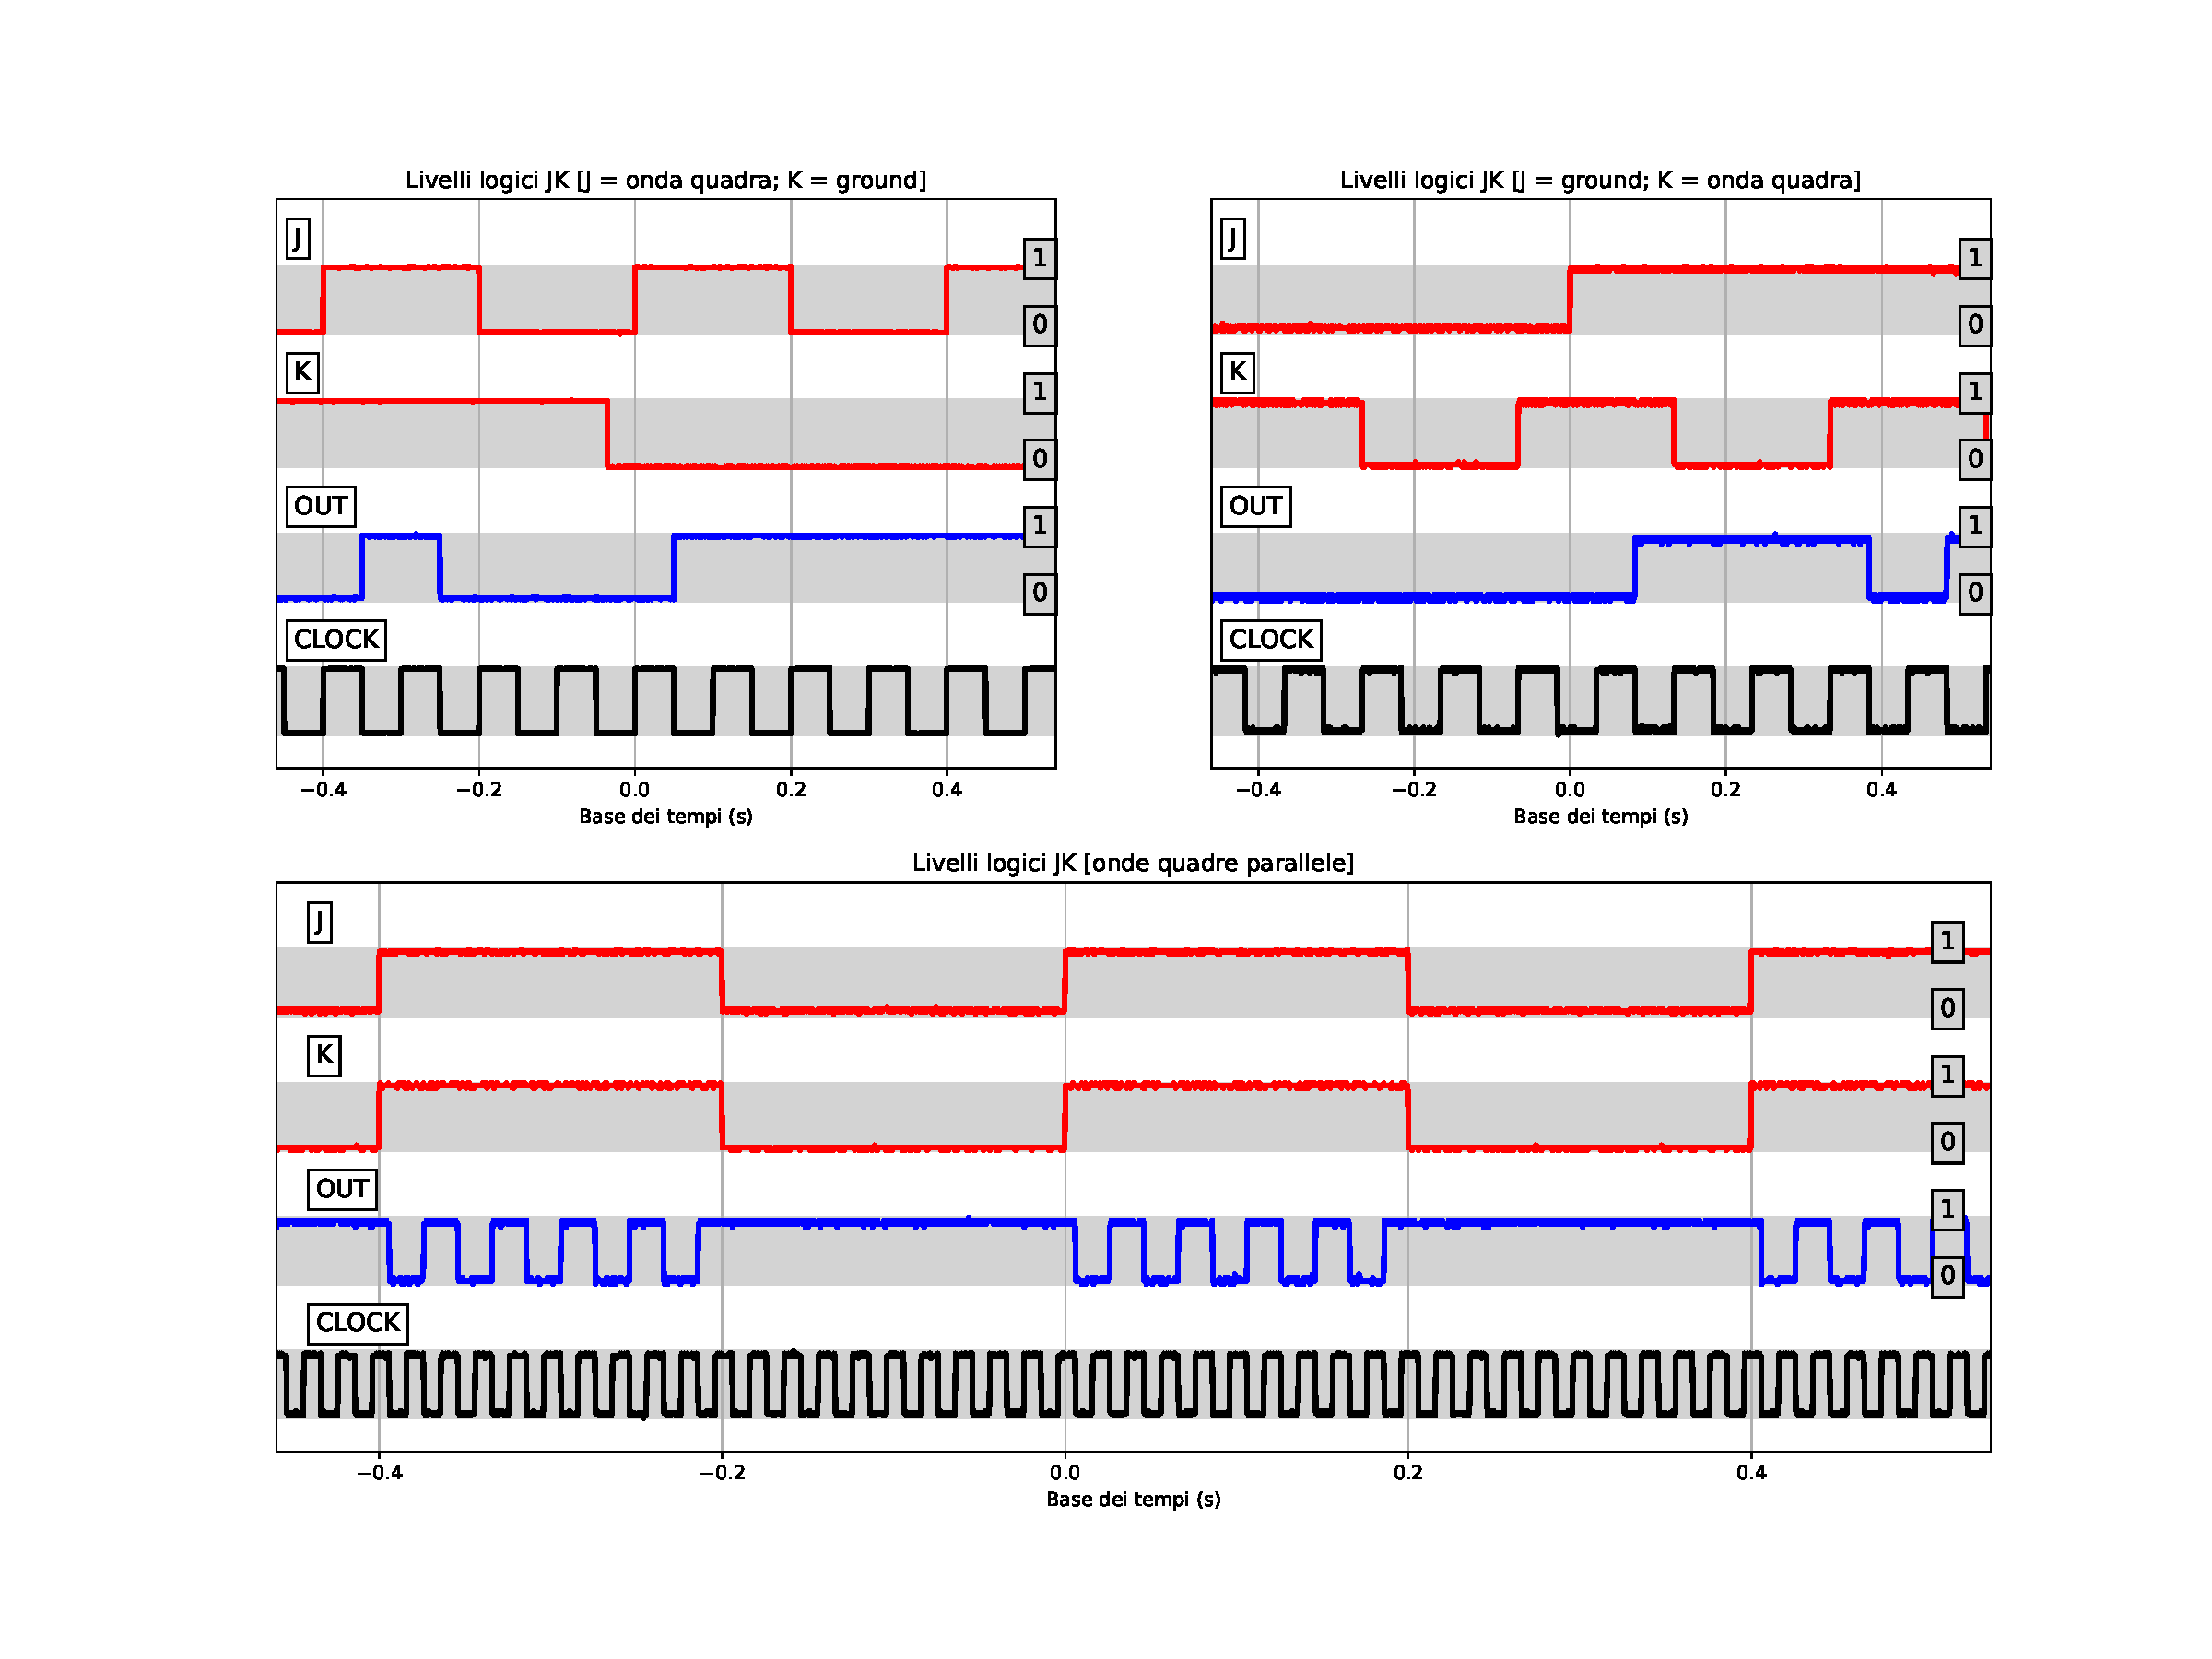
\includegraphics[width=0.48\textwidth]{analysis/output/JK-truth.pdf}
\caption{Verifica della tabella di verità di un flip-flop di tipo J-K}
\label{fig:graph_ring_oscillator}
\end{center}
\end{figure}

%%%%%%%%%%%%%%%%%%%%%%%%%%%%%%%%%%%%%%%%%%%%%%%%%%%%%%%%

\section{Verifica del funzionamento del ring oscillator realizzato con inverter}
Come anticipato nel paragrafo di descrizione degli integrati, il dispositivo SN74LS04 che implementa 6 porte NOT presenta un tempo di commutazione non trascurabile al variare del livello logico del segnale in ingresso alle alte frequenze e questo, se realizziamo una catena di porte OR, darà origine ad un ritardo di propagazione del segnale in ogni porta. 
Questo effetto porta a conseguenze interessanti se si realizza un anello chiuso con un numero dispari di inverters, nel nostro caso 7 suddivisi su due integrati. Si osserva infatti, collegando una sonda dell'oscilloscopio ad un punto arbitrario, che alimentando gli inverter le uscite cominciano ad oscillare liberamente con una forma d'onda che ricorda un'onda triangolare distorta con un periodo proporzionale al ritardo introdotto da ogni porta e al numero delle porte. Si sottolinea che il circuito risultante è un vero e proprio oscillatore, in quanto è in grado di produrre un'uscita periodica a partire da ingressi costanti nel tempo e non necessita di alcun innesco esterno se non quello dato dal rumore.

\begin{figure}[H]%[!ht]
\begin{center}
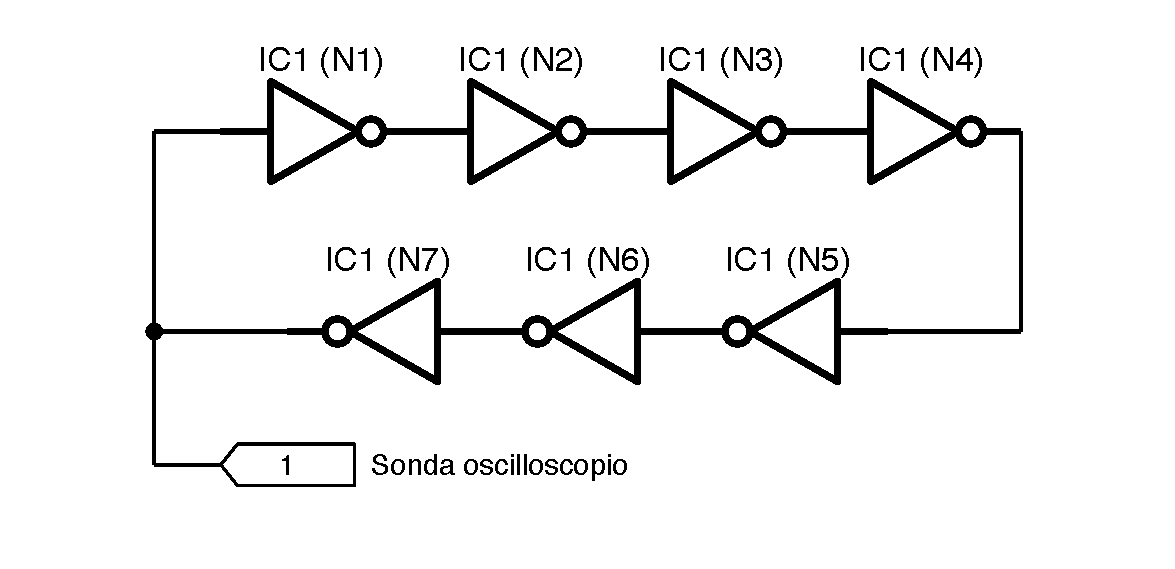
\includegraphics[width=0.40\textwidth]{sch-simulations/digital/output/ring-osc-logic.pdf}
\caption{Circuito equivalente dell'oscillatore ad anello}
\label{fig:circuit_ring_oscillator}
\end{center}
\end{figure}

Tra il ritardo di propagazione (t), il numero delle porte (n) e la frequenza della tensione oscillante generata (f) vale la presente relazione: 
\begin{math}
f = \frac{1}{2tn}
\end{math}
In laboratorio è stata acquisita la forma d'onda seguente, la cui frequenza risulta essere f = (12.66 $\pm$ 0.01) MHz, corrispondente ad un ritardo di propagazione medio tra gli inverter t = (5.6428 $\pm$ 0.0007) ns.


\begin{figure}[H]%[!ht]
\begin{center}
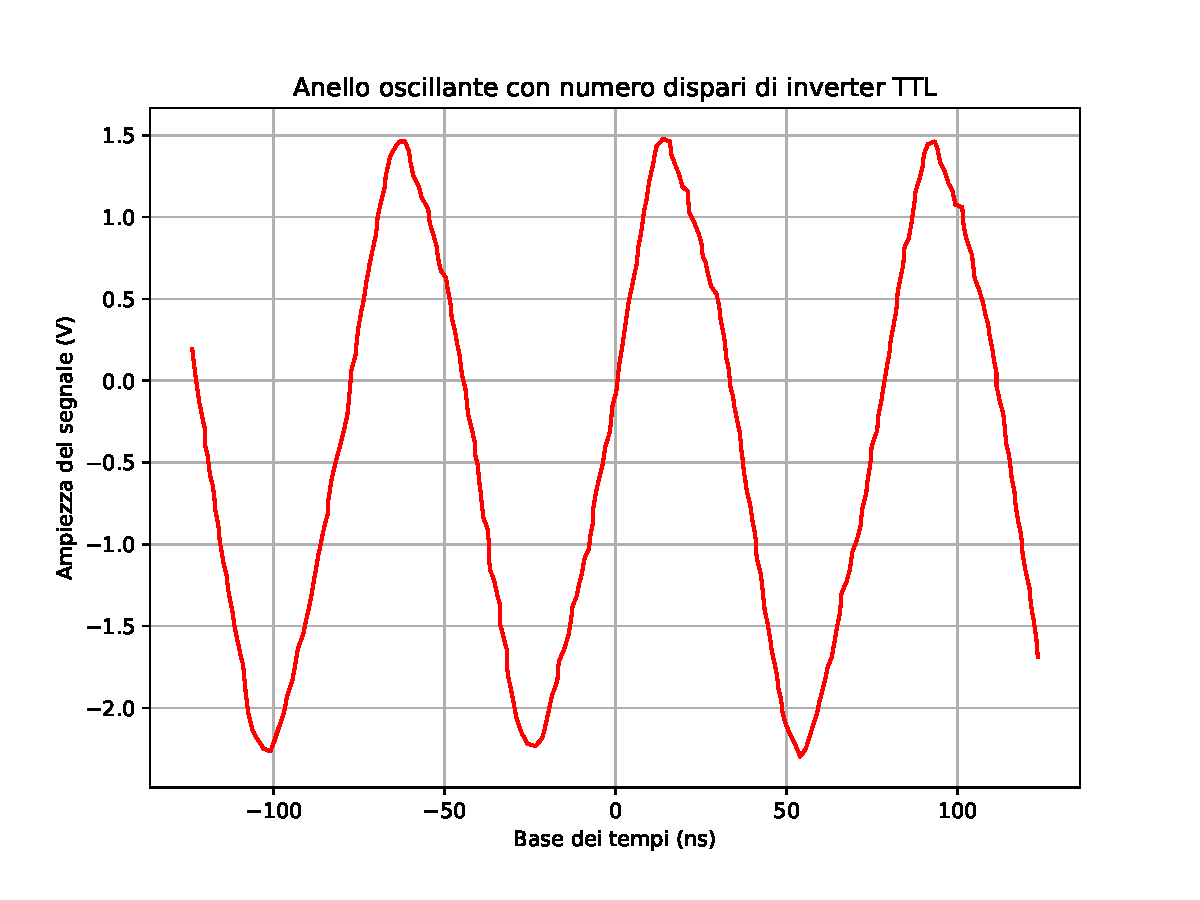
\includegraphics[width=0.52\textwidth]{analysis/output/oscillating-ring.pdf}
\caption{Forma d'onda generata dall'anello di inverter}
\label{fig:graph_ring_oscillator}
\end{center}
\end{figure}


Oscillatori di questo tipo sono utili per numerose applicazioni che spaziano dai VCO (voltage controller oscillators) dei phased-locked-loops (PLL) impiegati per generare il clock di tutte le moderne CPU fino alla generazione di numeri casuali sfruttando il jitter.

%%%%%%%%%%%%%%%%%%%%%%%%%%%%%%%%%%%%%%%%%%%%%%%%%%%%%%%%

\section{Realizzazione di un ADC SAR a 4 bit}

\subsection{Descrizione generale e specifiche tecniche desiderate}
Dopo aver preso in esame alcuni circuiti logici fondamentali, verrà ora affrontata la progettazione, calibrazione e verifica di un ADC ad approssimazioni successive (SAR) con risoluzione di 4 bit, rappresentato nello schema in figura \ref{fig:circuit_sarCompleteSchematic}. Questa tipologia di convertitori analogico - digitali è molto diffusa, sia in circuiti integrati stand alone (per esempio \textit{Analog Devices AD4695} sia all'interno di microcontrollori (per esempio la serie \textit{STM32} della \textit{ST Microelectronics}) e consente di raggiungere un buon compromesso tra frequenza di campionamento e risoluzione.

Il convertitore SAR che verrà realizzato utilizza un registro di scorrimento a 8 bit, pertanto la frequenza di campionamento sarà pari a un ottavo della frequenza di clock che durante la caratterizzazione è stata posta al massimo a 10 KHz. In questo regime di funzionamento il convertitore si è sempre mostrato affidabile, mentre a frequenze maggiori gli amplificatori operazionali dello stadio analogico costituiscono il collo di bottiglia del sistema. Il convertitore ha un tempo di acquisizione dato dalla lunghezza della finestra in cui l'integato \textit{sample and hold} LF398 effettua il campionamento, pari a un periodo del clock.

Il convertitore si compone dei seguenti blocchi funzionali fondamentali (con riferimento allo schema in figura \ref{fig:circuit_sarCompleteSchematic}):
\begin{itemize}
    \item Un registro di scorrimento a 8 bit (U7) che permette di effettuare la scansione dei bit nel processo di confronto del segnale in ingresso ad approssimazioni successive, insieme a due circuiti di controllo implementati con porte NAND: il primo, basato su U8, genera il segnale di \textit{clear} che effettua il reset degli integrati TTL al termine del ciclo di conversione, mentre il secondo, basato su U9, inizializza l'ingresso del registro all'inizio di ogni ciclo di conversione.
    \item Una logica comprendente 4 porte AND implementate nell'integrato U5 che controllano 4 flip-flop di tipo J-K, implementati negli integrati U3 e U4. (MSB su U3). I flip-flop J-K vengono settati (J) in sequenza dalle uscite del registro di scorrimento e vengono resettati (K) quando viene settato il flip-flop successivo solamente se il circuito comparatore ha come complemento logico dell'uscita uno stato alto. Al termine di un ciclo del registro le uscite dei J-K rappresentano quindi il risultato della conversione.
    \item Uno stadio analogico che confronta il segnale in ingresso con la sua rappresentazione fornita dalle uscite dei J-K, composto da un DAC R-2R controllato da queste ultime la cui uscita viene confrontata mediante un OPA LM741 ad anello aperto (U2) con la tensione da campionare. L'uscita del comparatore pilota le porte AND che resettano i J-K mediante un transistor di interfaccia che garantisce sia la compatibilità dei livelli logici (l'uscita arriva a +15 V, mentre TTL prevede lo stato alto a +5 V), sia un più rapido fronte di commutazione. Lo stadio analogico può essere completato inserendo un circuito di \textit{sample and hold} a monte, pilotato dal registro a scorrimento.
\end{itemize}

\subsection{Verifica del circuito con registro di scorrimento e annessa logica di controllo}
Testo


\begin{figure}[H]%[!ht]
\begin{center}
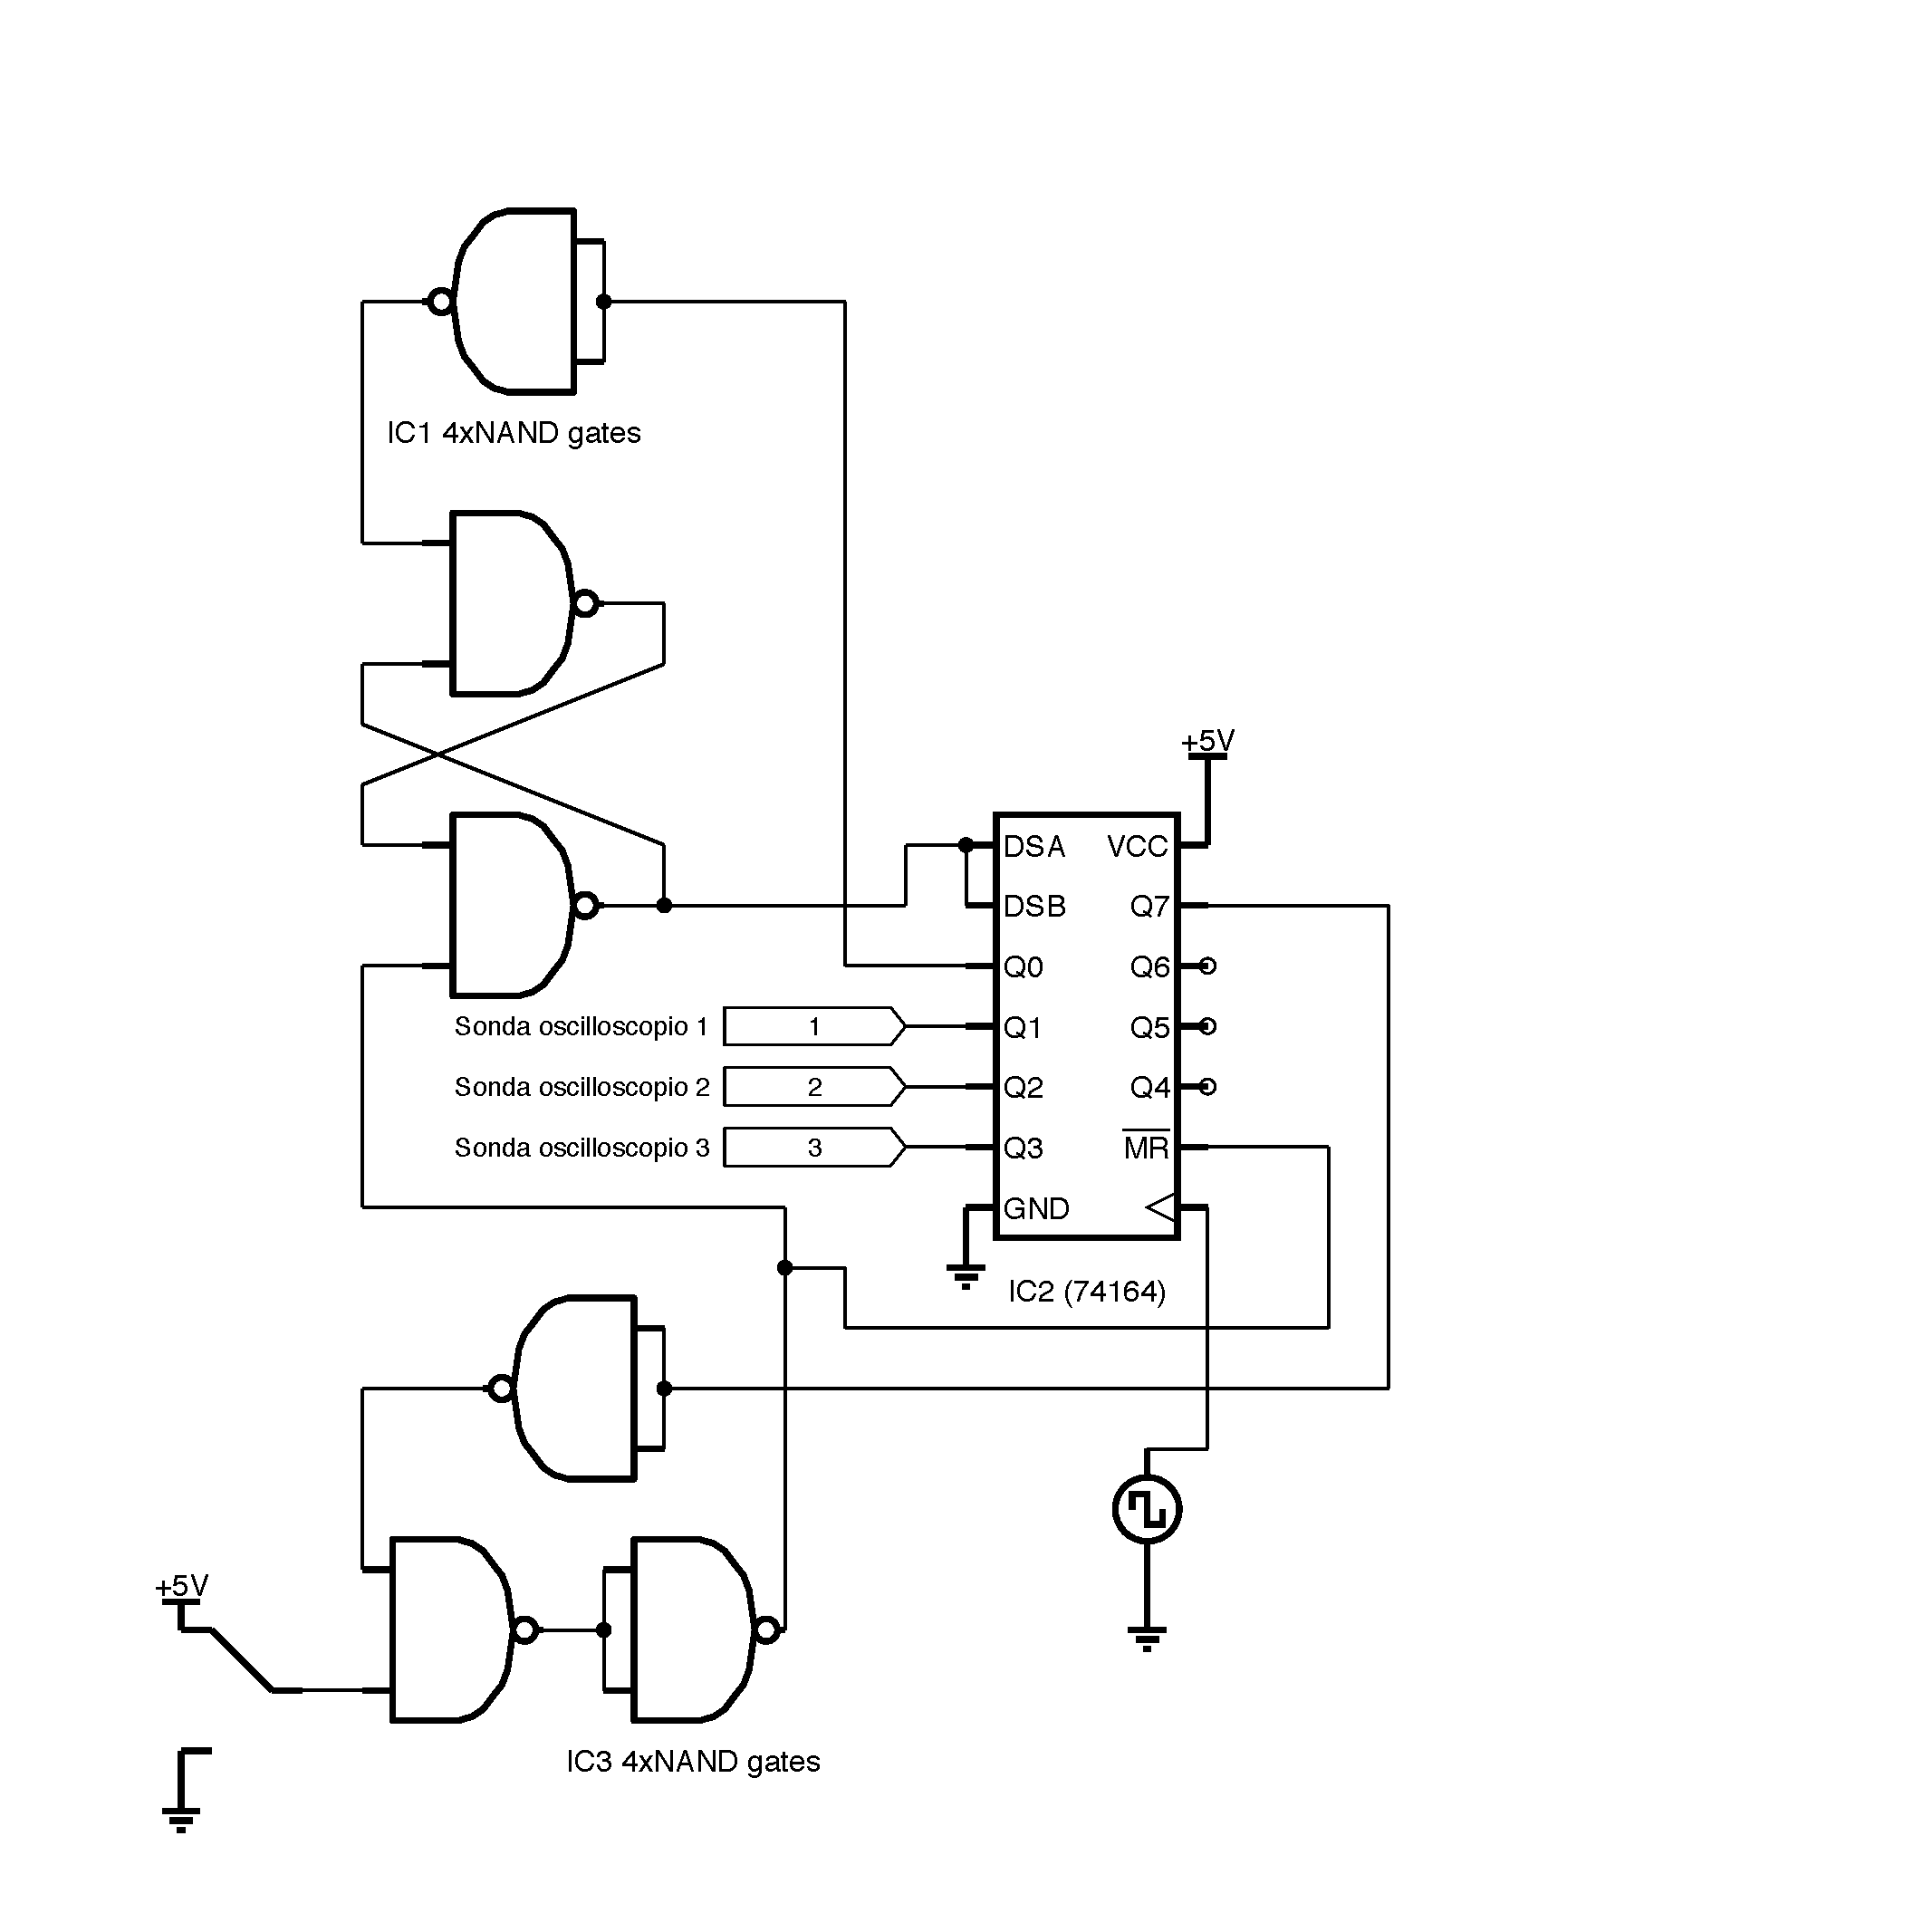
\includegraphics[width=0.50\textwidth]{sch-simulations/digital/output/shift-register.pdf}
\caption{Registro a scorrimento e circuito di controllo}
\label{fig:circuit_shift_register}
\end{center}
\end{figure}



\subsection{Verifica del circuito di pilotaggio del DAC (J-K) e dello stadio analogico}
Testo

\begin{figure}[H]%[!ht]
\begin{center}
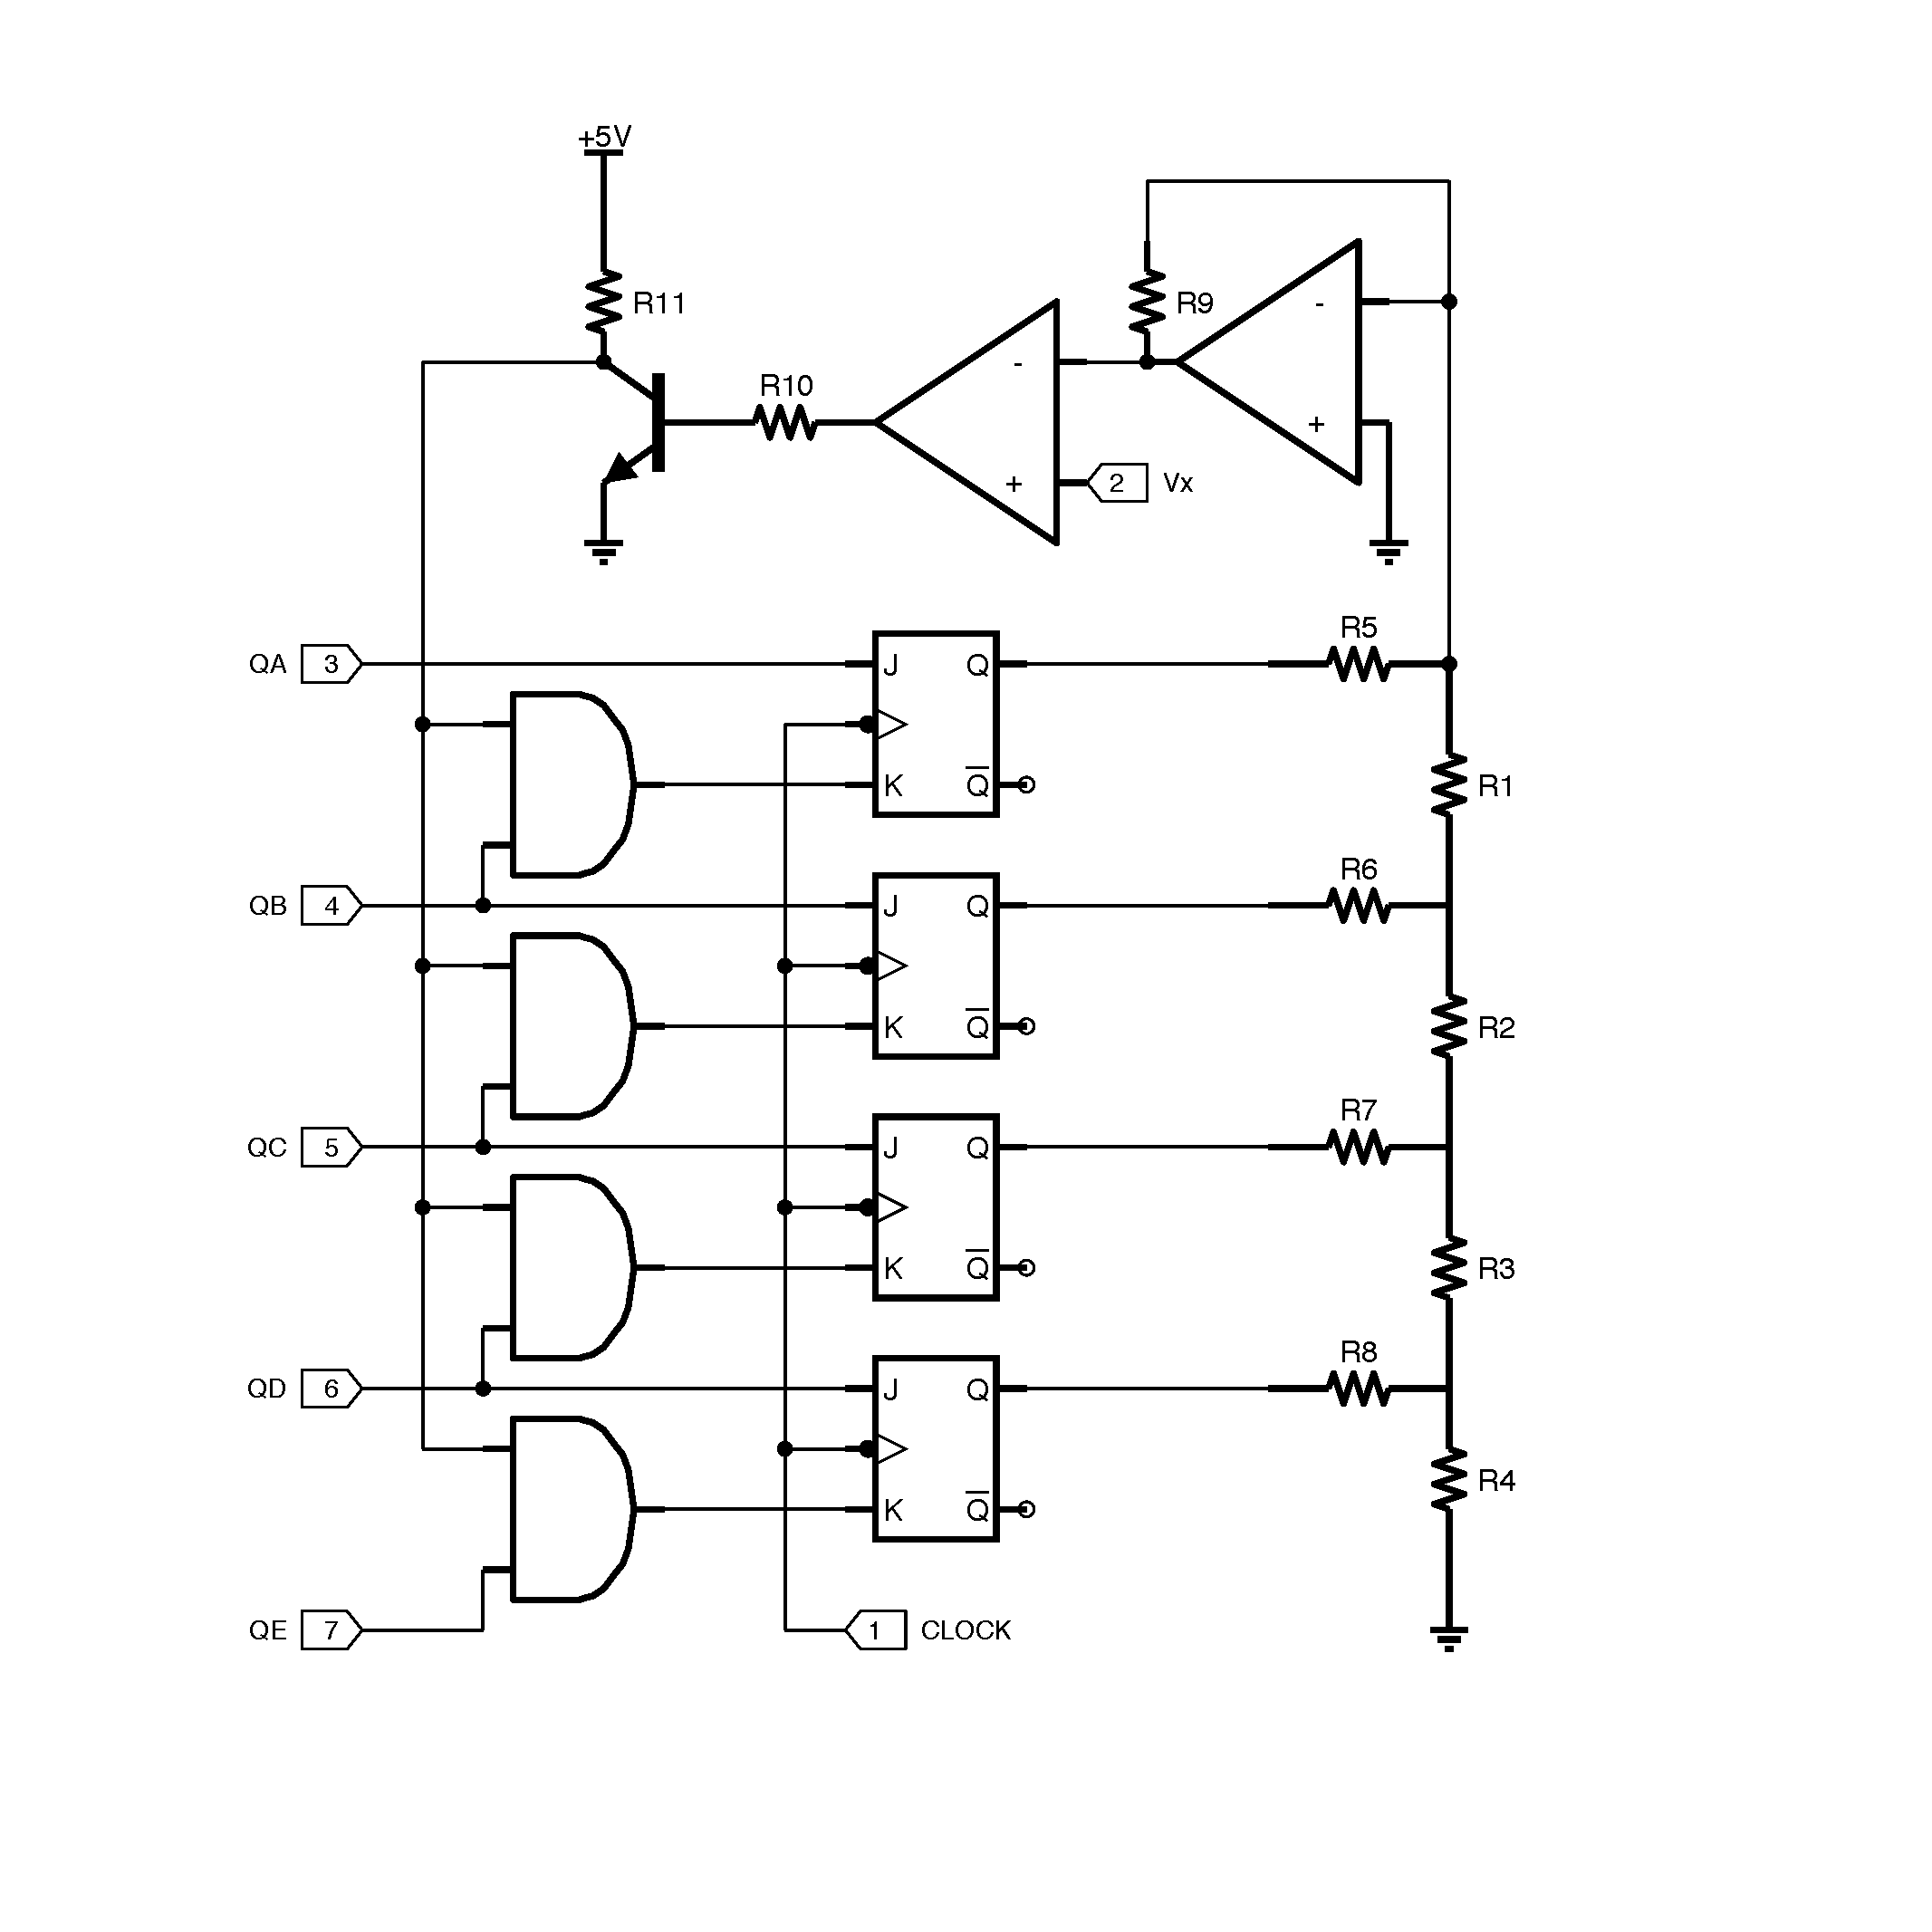
\includegraphics[width=0.40\textwidth]{sch-simulations/digital/output/DAC.pdf}
\caption{DAC}
\label{fig:circuit_DAC}
\end{center}
\end{figure}

\begin{figure}[H]%[!ht]
\begin{center}
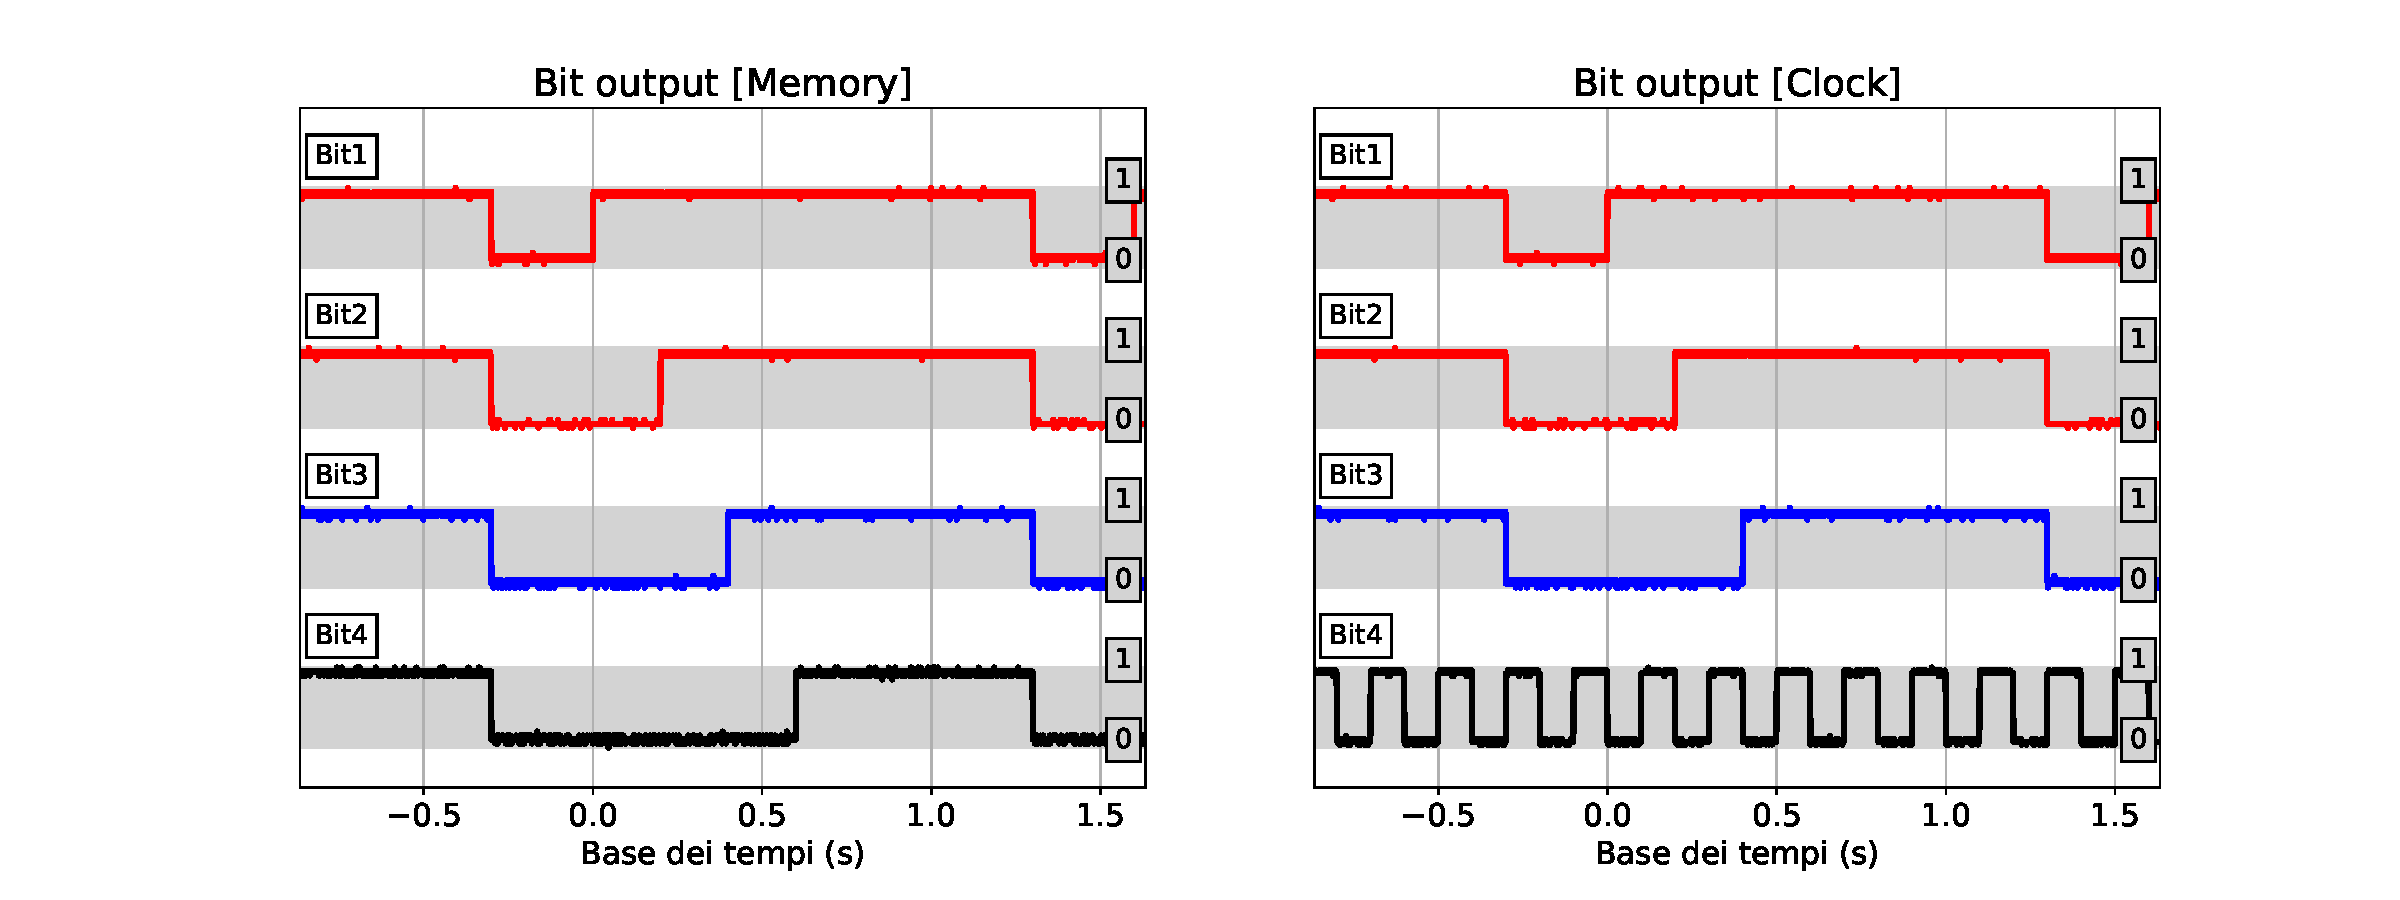
\includegraphics[width=0.40\textwidth]{analysis/output/cumulative_BIT.pdf}
\caption{memoria bit}
\label{fig:cumulative_BIT}
\end{center}
\end{figure}


\begin{figure}[H]%[!ht]
\begin{center}
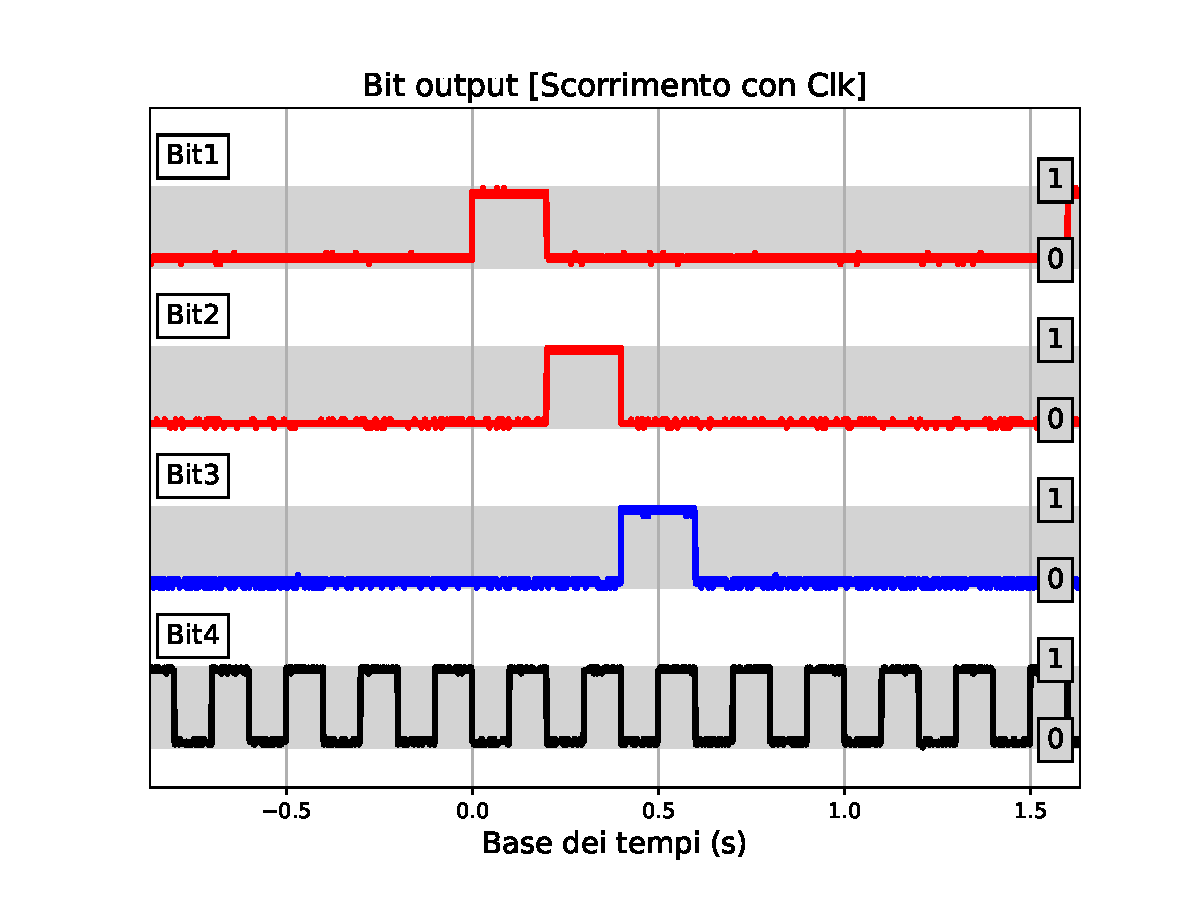
\includegraphics[width=0.40\textwidth]{analysis/output/BIT-shift-clk.pdf}
\caption{circuito di scorrimento}
\label{fig:BIT_shift_clk}
\end{center}
\end{figure}

\begin{figure}[H]%[!ht]
\begin{center}
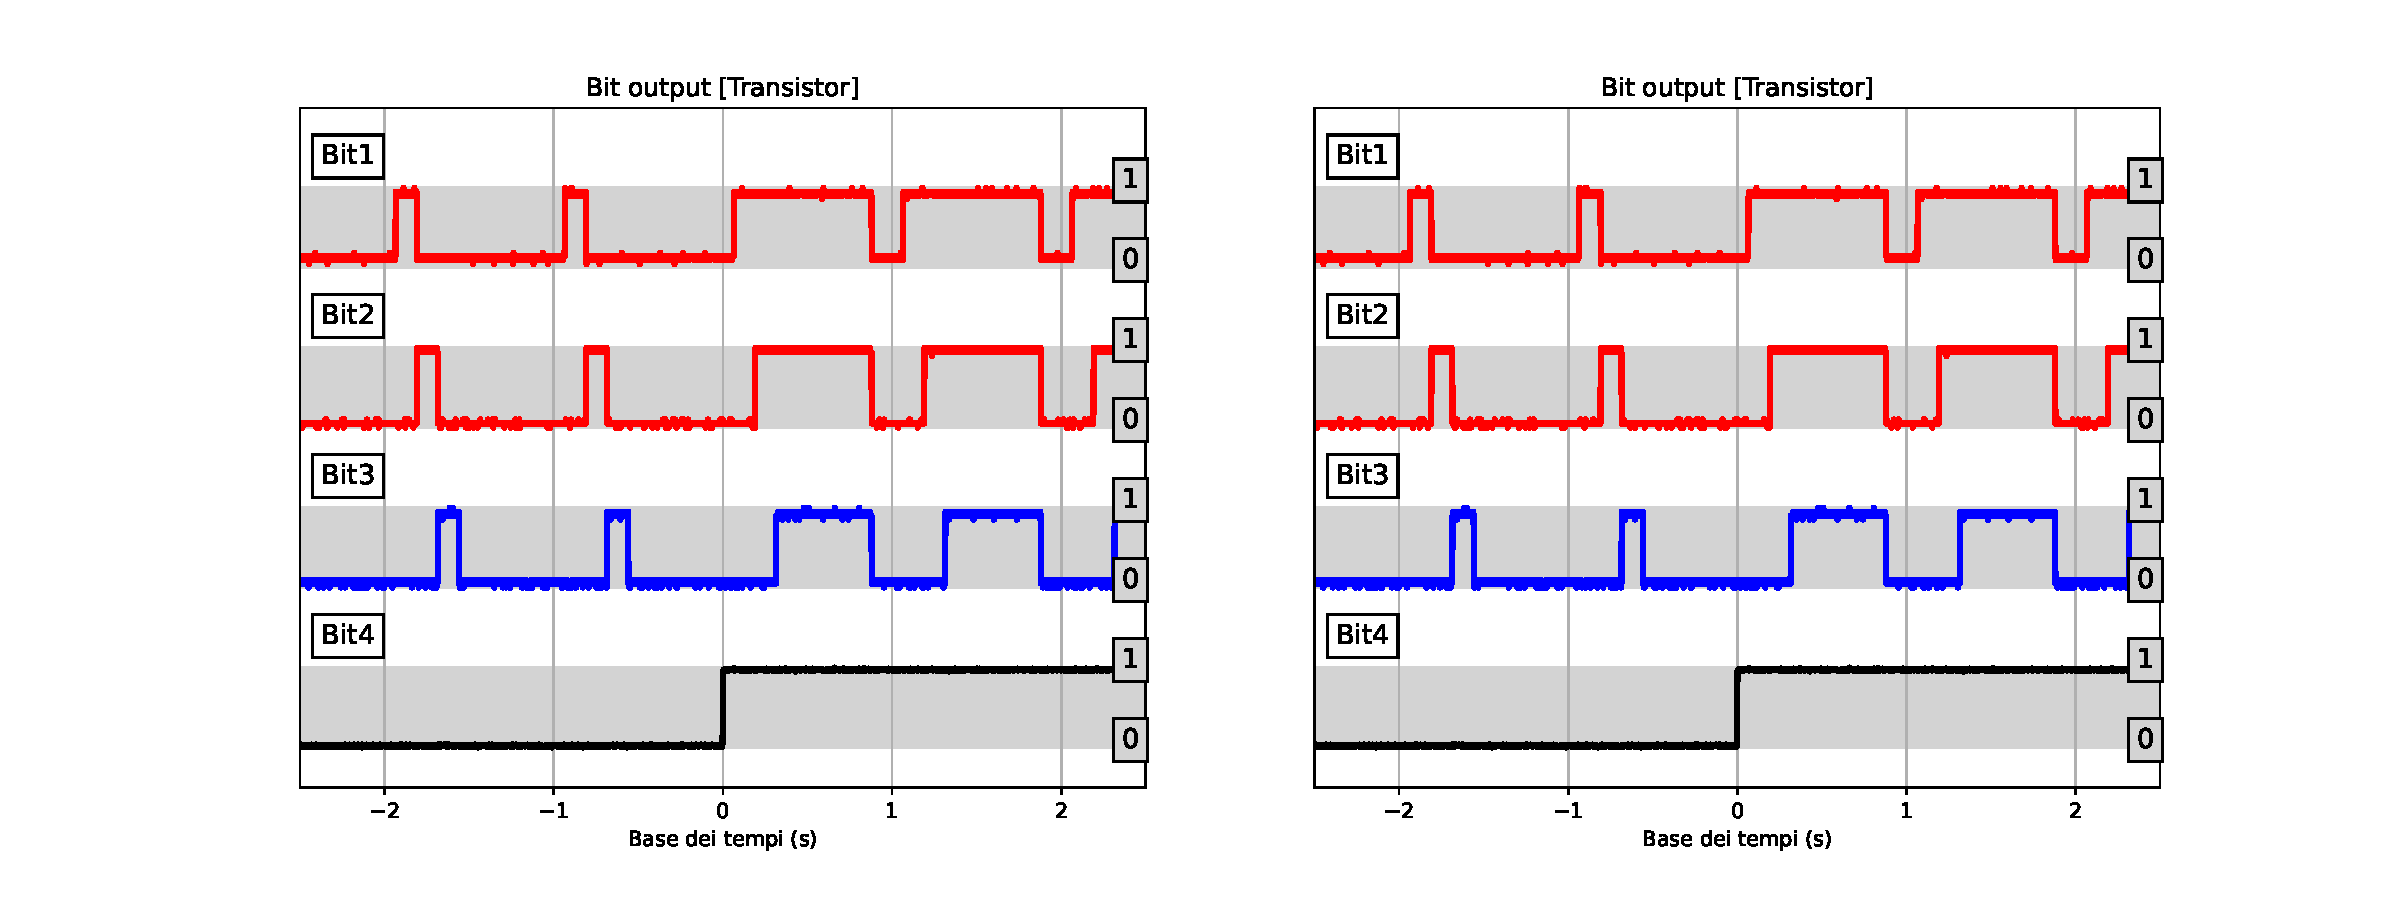
\includegraphics[width=0.40\textwidth]{analysis/output/cumulative_BIT_with_transistor.pdf}
\caption{BIT con transistor}
\label{fig:BIT_with_transistor}
\end{center}
\end{figure}




\subsection{Caratteristica di trasferimento del transistor di interfaccia}
Testo

\begin{figure}[H]%[!ht]
\begin{center}
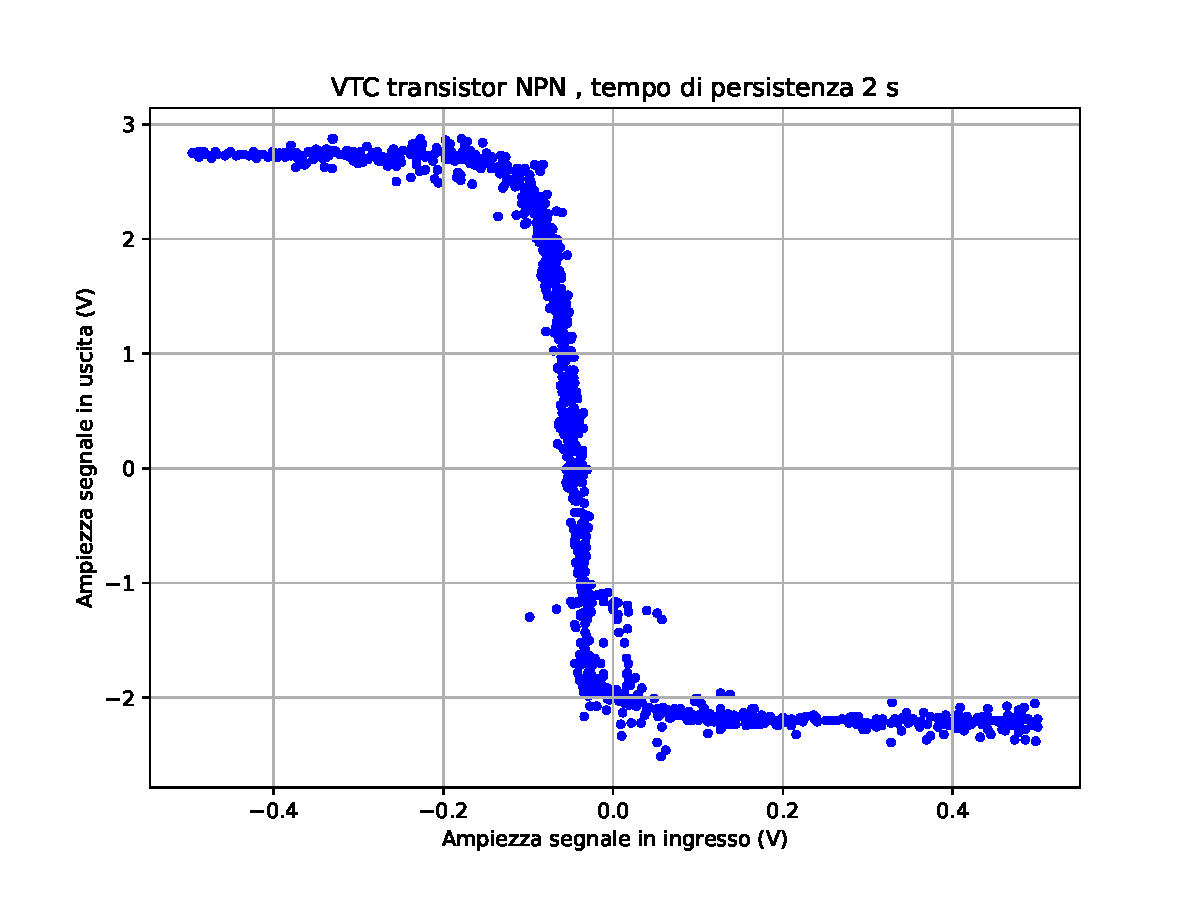
\includegraphics[width=0.45\textwidth]{analysis/output/NPN-XY.pdf}
\caption{Caratteristica di trasferimento in tensione base-collettore del transistor di interfaccia.}
\label{fig:inverter_ring_xy}
\end{center}
\end{figure}


\subsection{Caratteristiche del segnale di \textit{clear}}
Testo

\begin{figure}[H]%[!ht]
\begin{center}
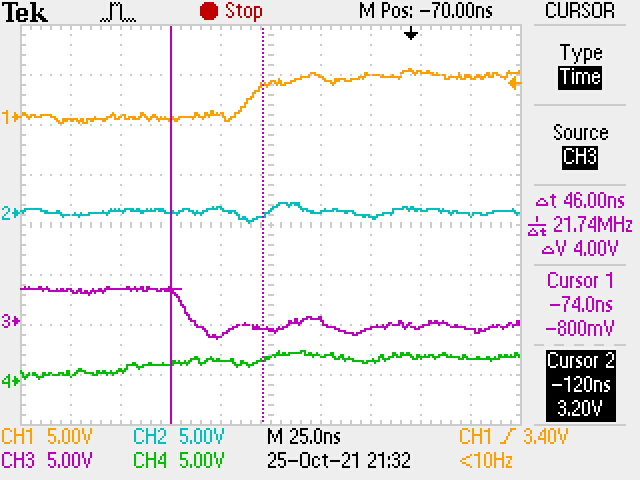
\includegraphics[width=0.45\textwidth]{data-source/25-10-21/DeltaT-clear.JPG}
\caption{Ritardo di propagazione attraverso i circuiti logici di U8 del segnale di clear}
\label{fig:inverter_ring_xy}
\end{center}
\end{figure}

%%%%%%%%%%%%%%%%%%%%%%%%%%%%%%%%%%%%%%%%%%%%%%%%%%%%%%%%%%%%%

\section{Calibrazione del DAC}

\begin{figure}[t]%[t]
\centering
\begin{center}
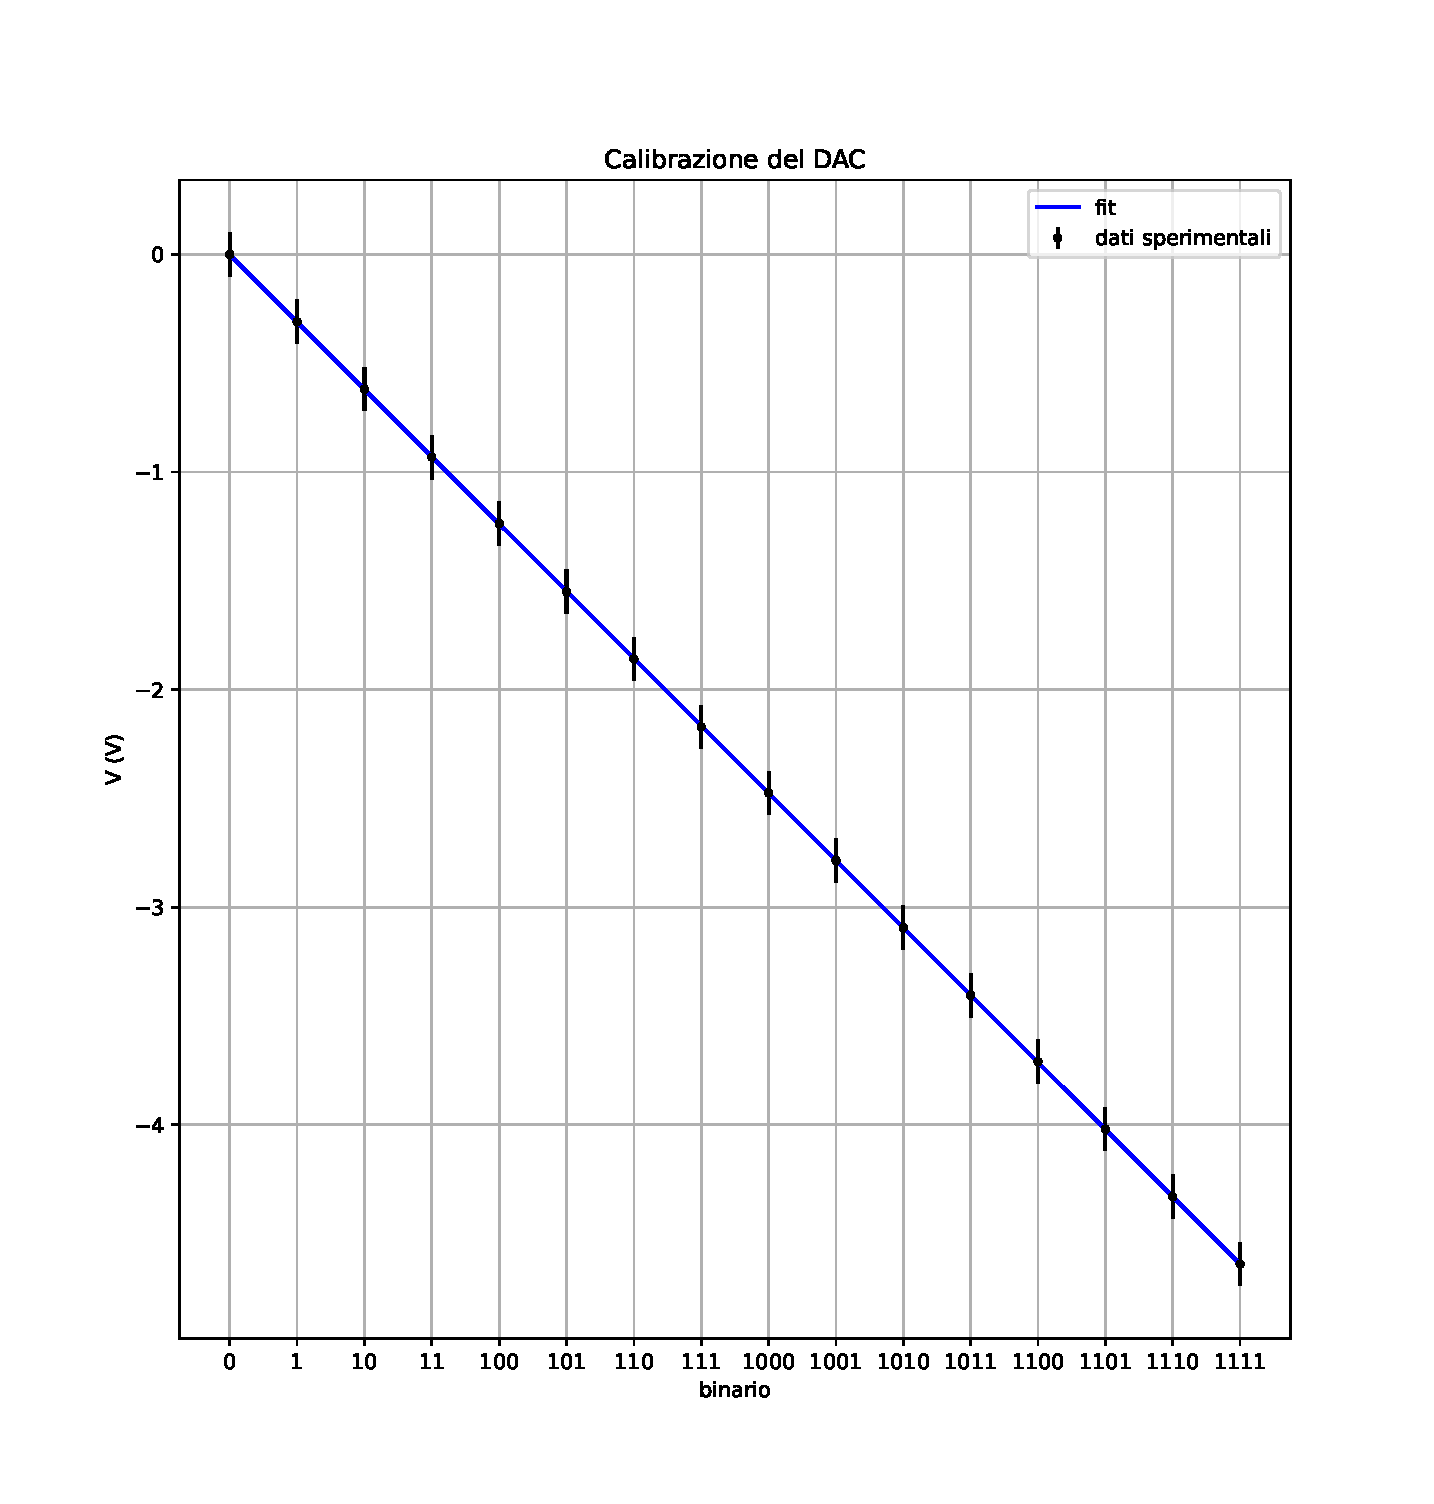
\includegraphics[width=0.51\textwidth]{analysis/output/calibrazione_dac.pdf}
\end{center}
\caption{Retta di calibrazione del DAC, i punti corrispondono alle tensioni misurate all'uscita quando i bit di ingresso vengono portati ai livelli logici rappresentati sull'asse orizzontale.}
\label{fig:graph_calibrazione_dac}
\end{figure}

$ m = -0.211 \pm 0.001 $ \\
$ q = -0.01 \pm 0.01 \ V $ \\
$ \chi^{2} = 0.006 $ \\

\ref{tab:calibrazione_dac}

%%%%%%%%%%%%%%%%%%%%%%%%%%%%%%%%%%%%%%%%%%%%%%%%%%%%%%%%%%%%%

\section{Campionamento di tensioni continue e calibrazione dell'ADC}

\begin{figure}[t]%[t]
\centering
\begin{center}
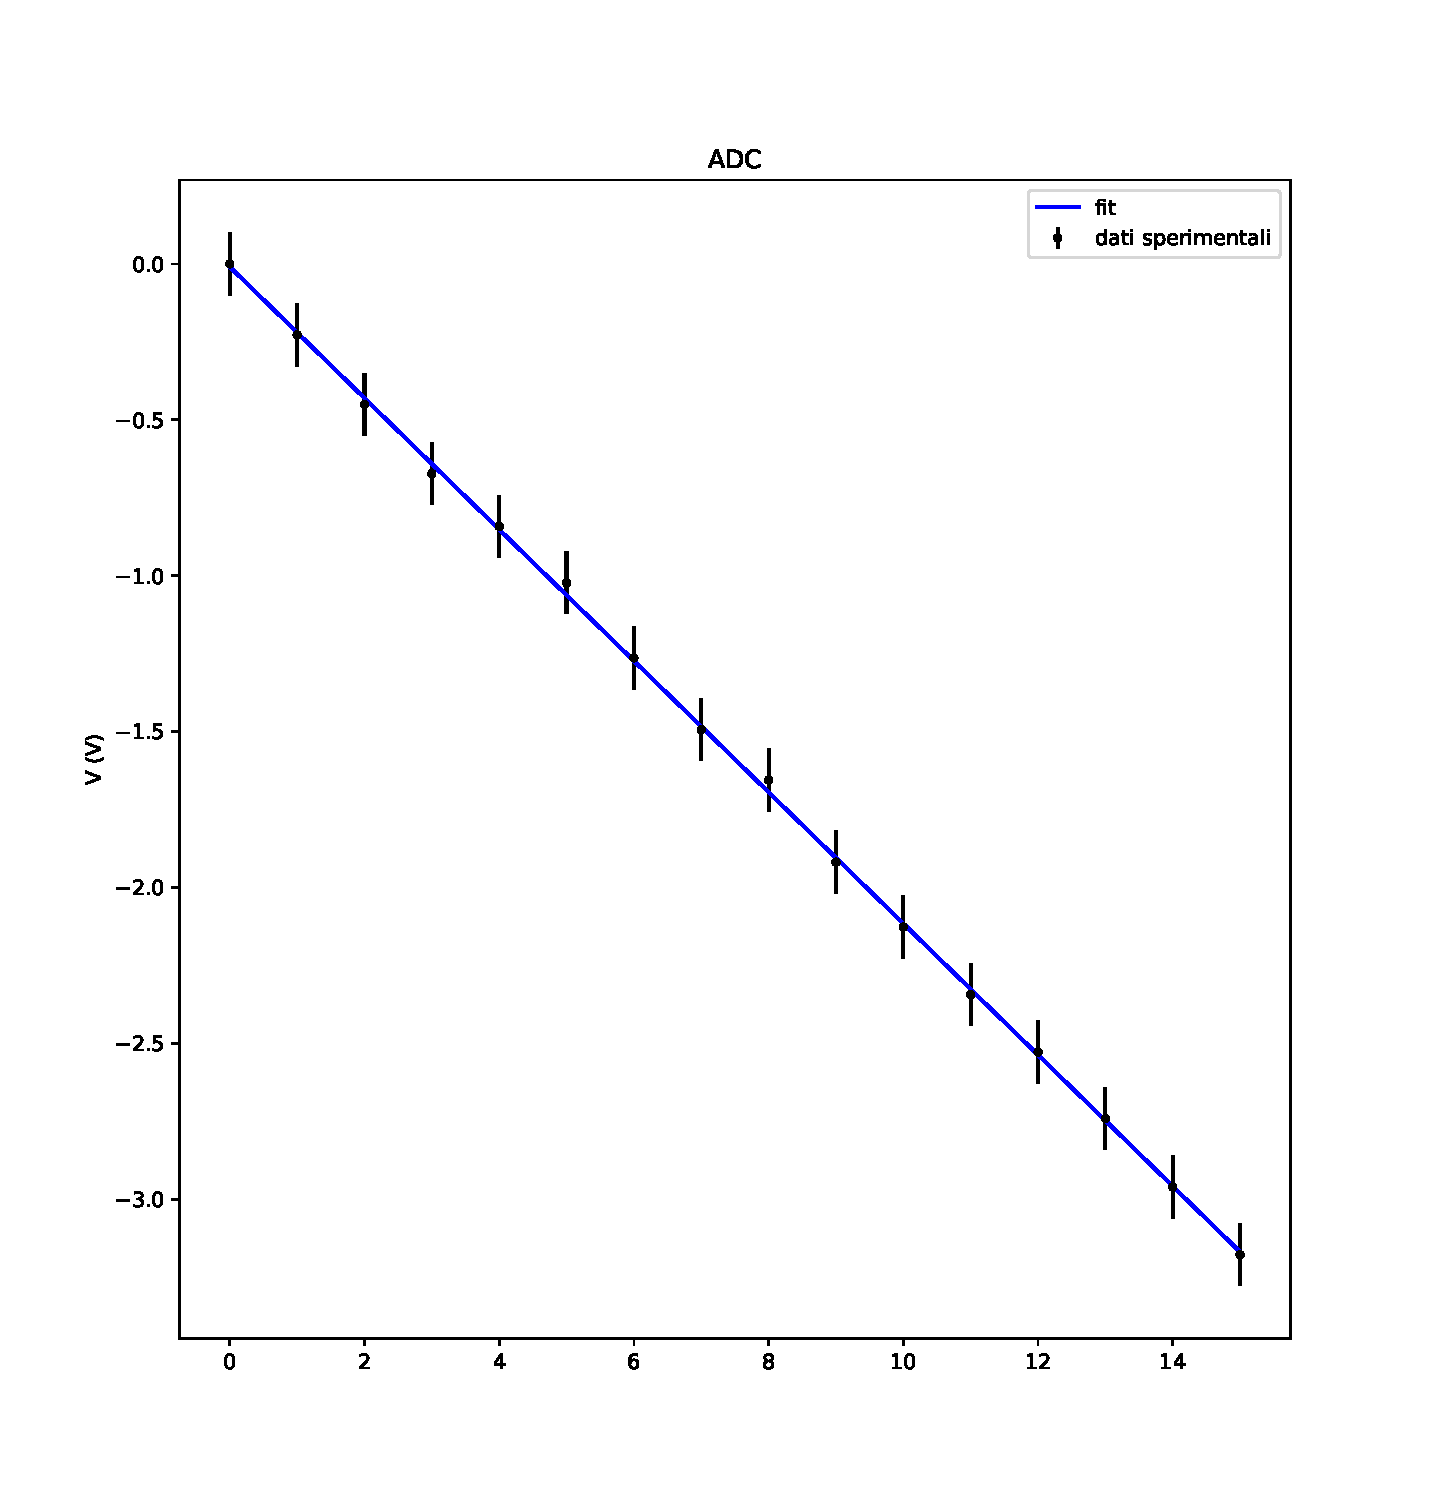
\includegraphics[width=0.51\textwidth]{analysis/output/calibrazione_adc.pdf}
\end{center}
\caption{Retta di calibrazione dell'ADC, i punti corrispondono alle soglie in cui cambia il codice binario restituito facendo variare la tensione in ingresso dal valore più negativo fino a 0 V.}
\label{fig:graph_calibrazione_adc}
\end{figure}

$ m = -0.3092 \pm 0.0001 $ \\
$ q = -0.02 \pm 0.01 \ V$ \\
$ \chi^{2} = 0.57 $ \\

\ref{tab:calibrazione_adc}

\begin{figure*}[t]%[t]
\centering
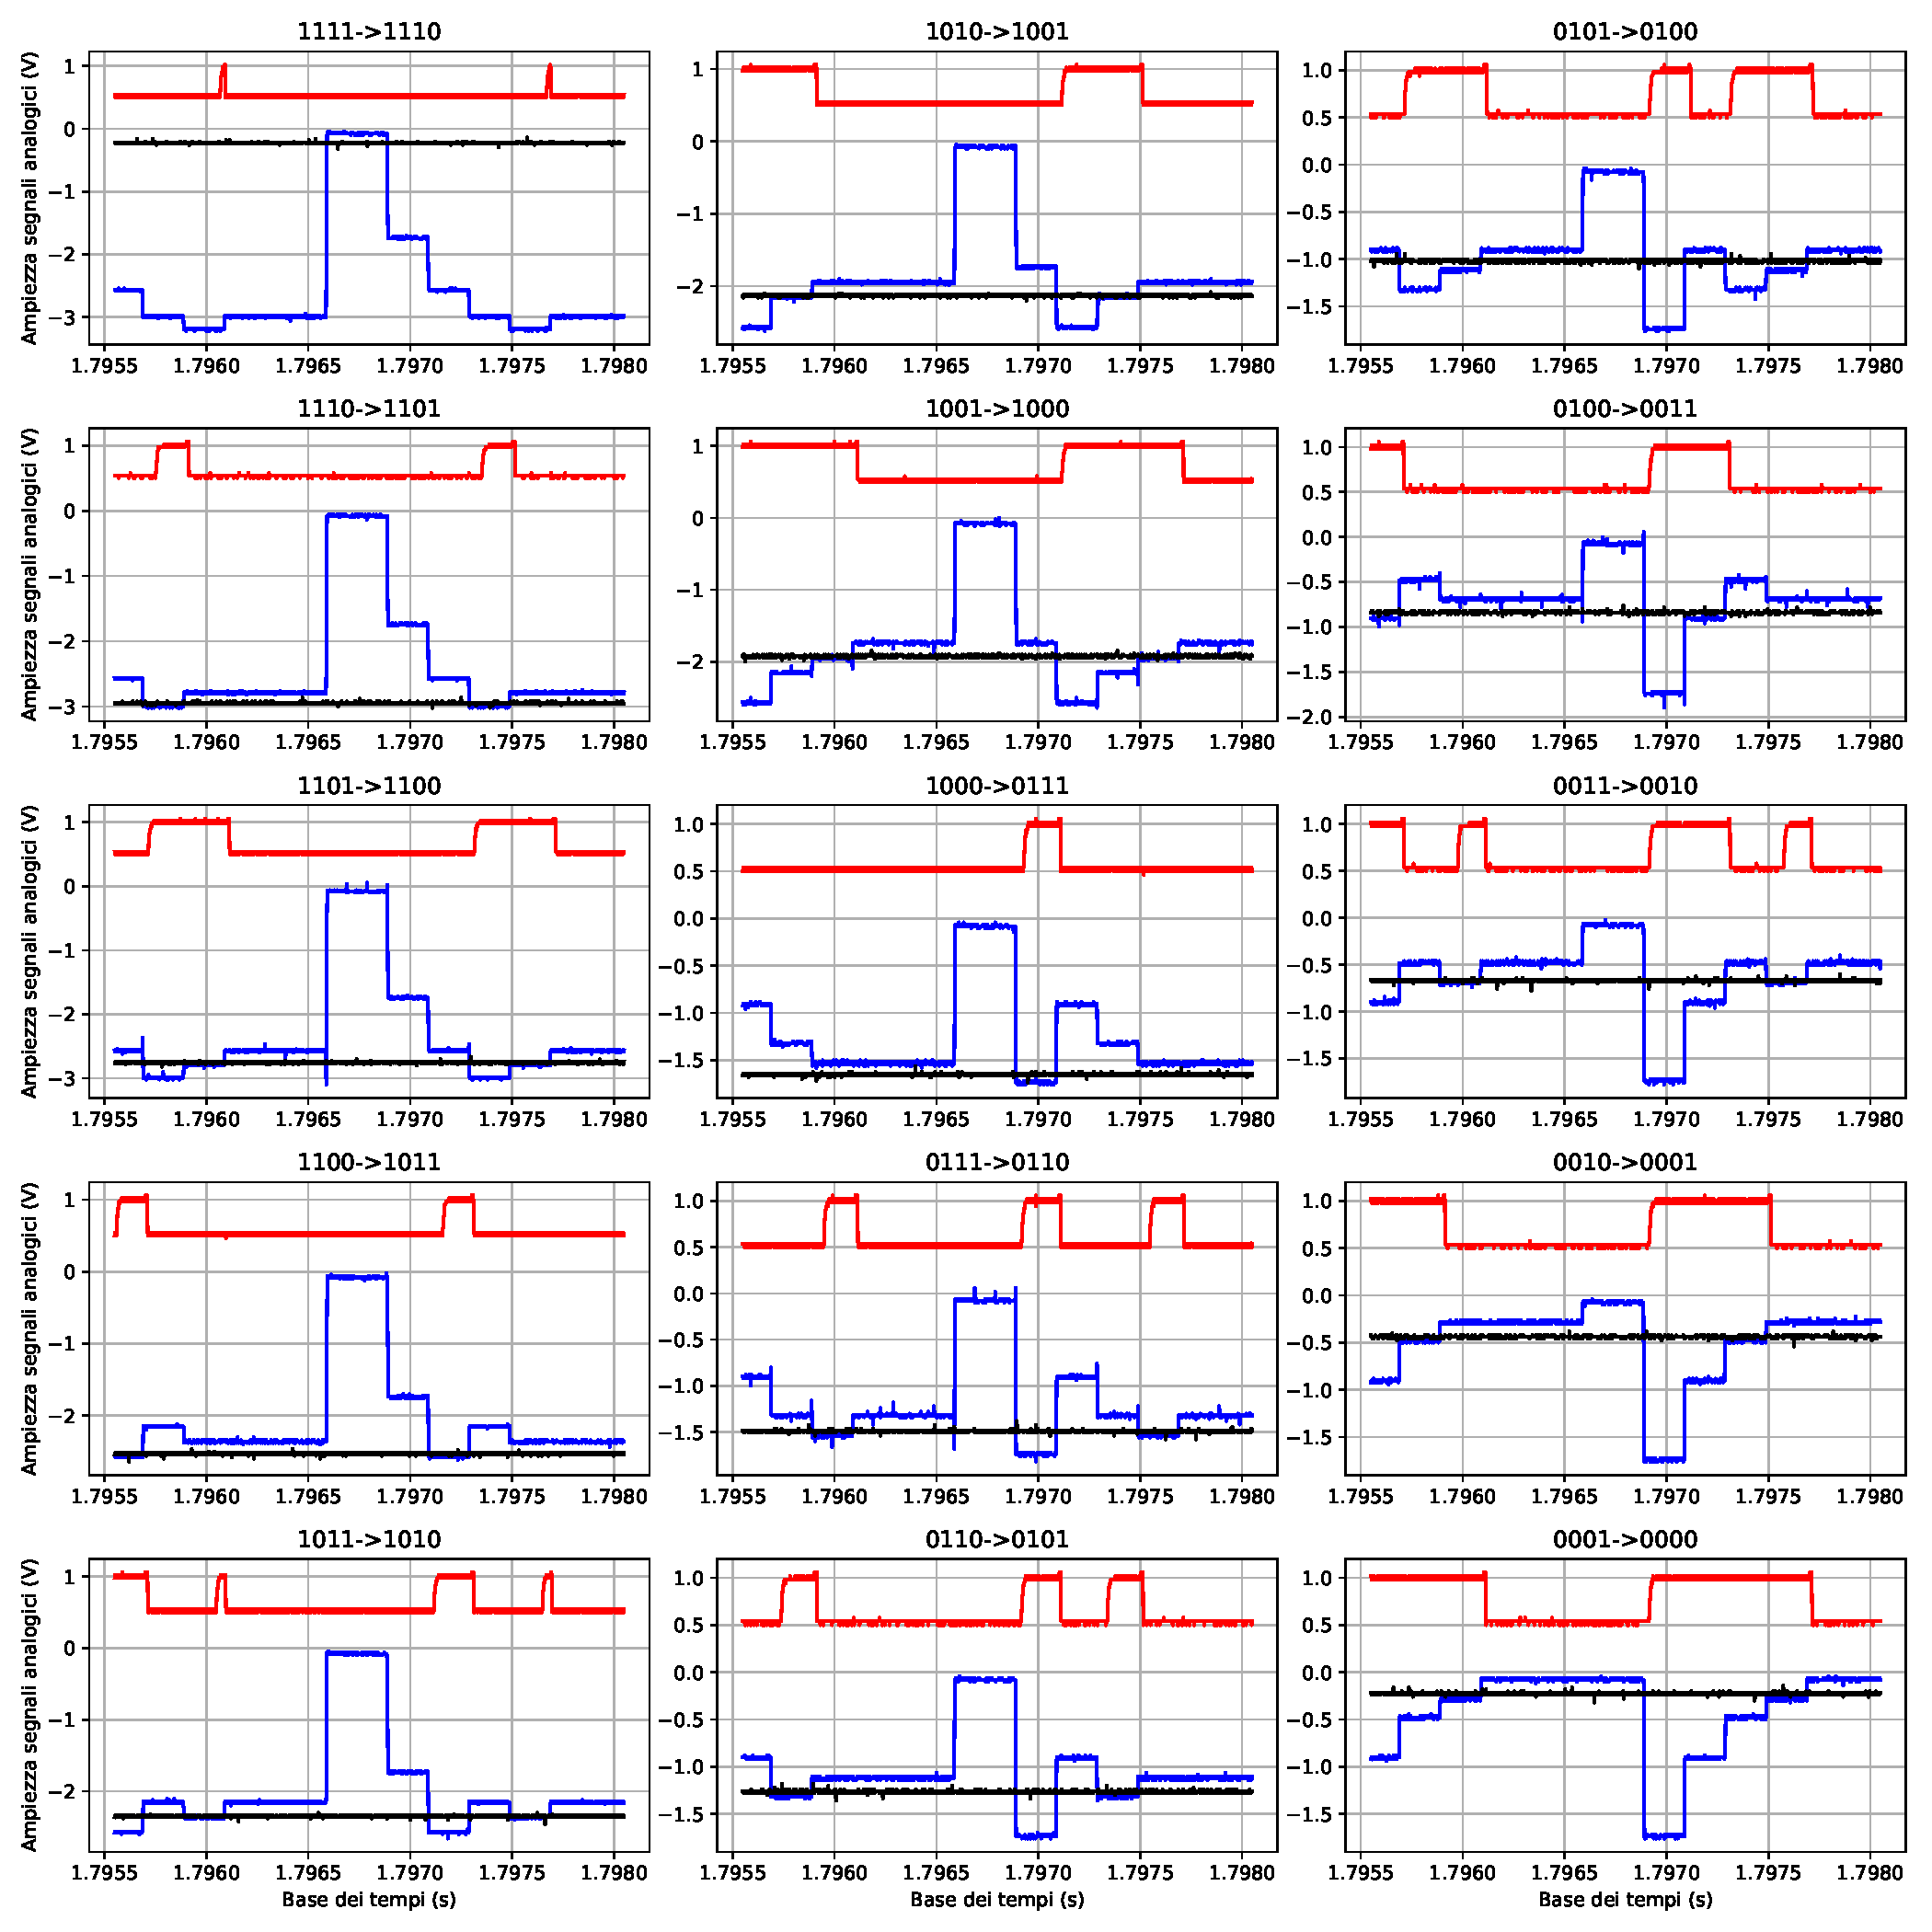
\includegraphics[trim = {30 0 50 0}, width=0.95\textwidth]{analysis/output/calibration.pdf}
\caption{Calibrazione dell'ADC}
\label{fig:waveforms_no_sh_scope}
\end{figure*}

%%%%%%%%%%%%%%%%%%%%%%%%%%%%%%%%%%%%%%%%%%%%%%%%%%%%%%%%%%%%%
\section{Campionamento di tensioni variabili}
Testo

\begin{figure}[H]%[!ht]
\begin{center}
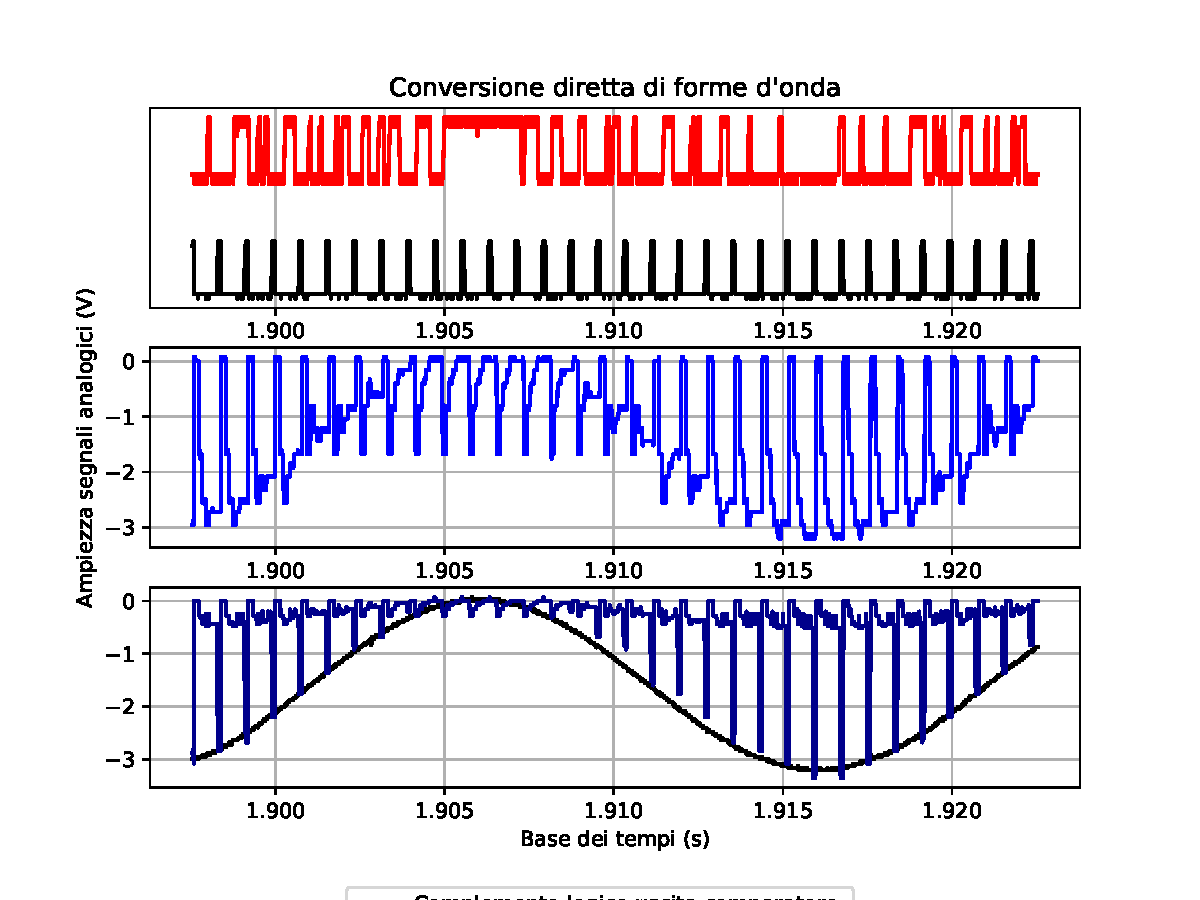
\includegraphics[trim = {0 25 0 0},clip, width=0.50\textwidth]{analysis/output/direct_aq_waveforms.pdf}
\caption{Didascalia}
\label{fig:circuit_DAC}
\end{center}
\end{figure}

\begin{figure}[H]%[!ht]
\begin{center}
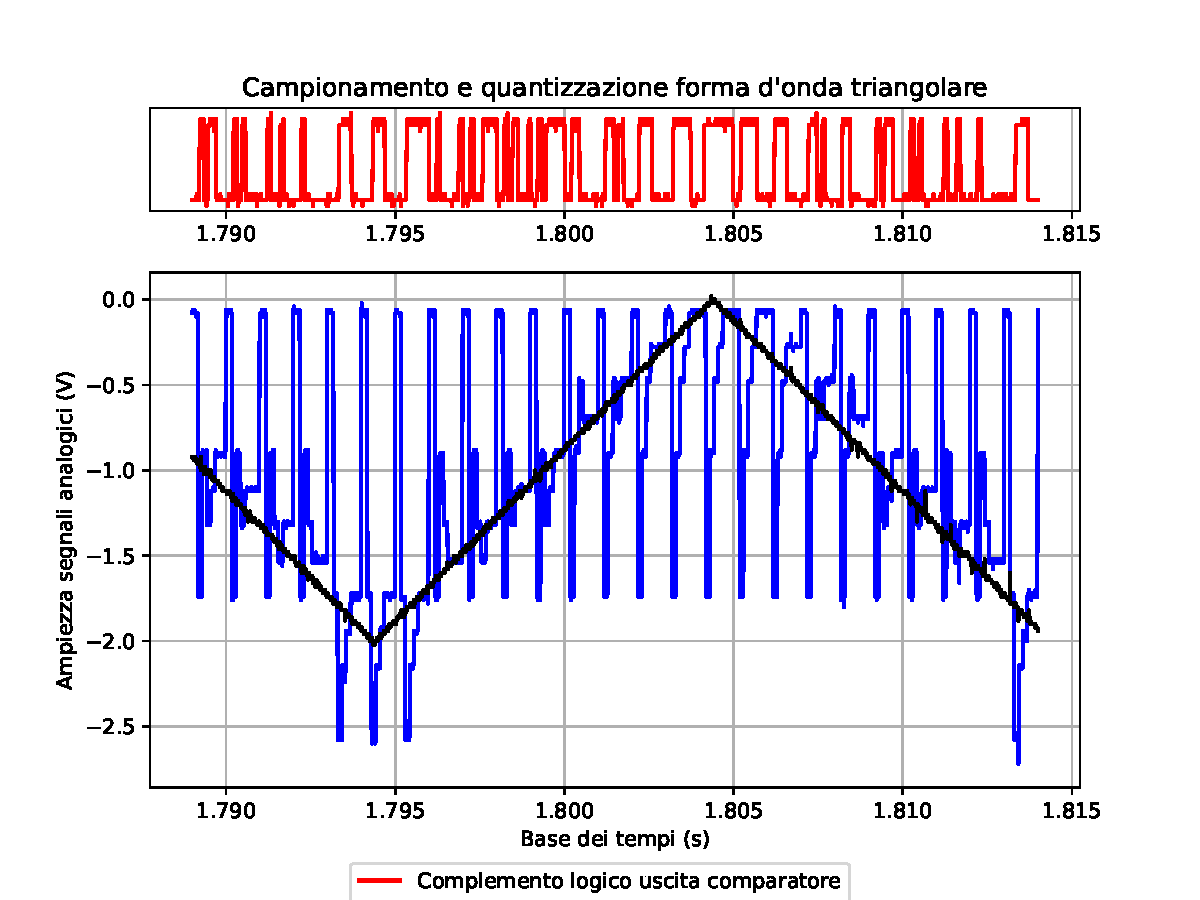
\includegraphics[trim = {0 25 0 0},clip, width=0.50\textwidth]{analysis/output/triangle_wave_aq.pdf}}
\caption{Didascalia}
\label{fig:circuit_DAC}
\end{center}
\end{figure}

\begin{figure}[H]%[!ht]
\begin{center}
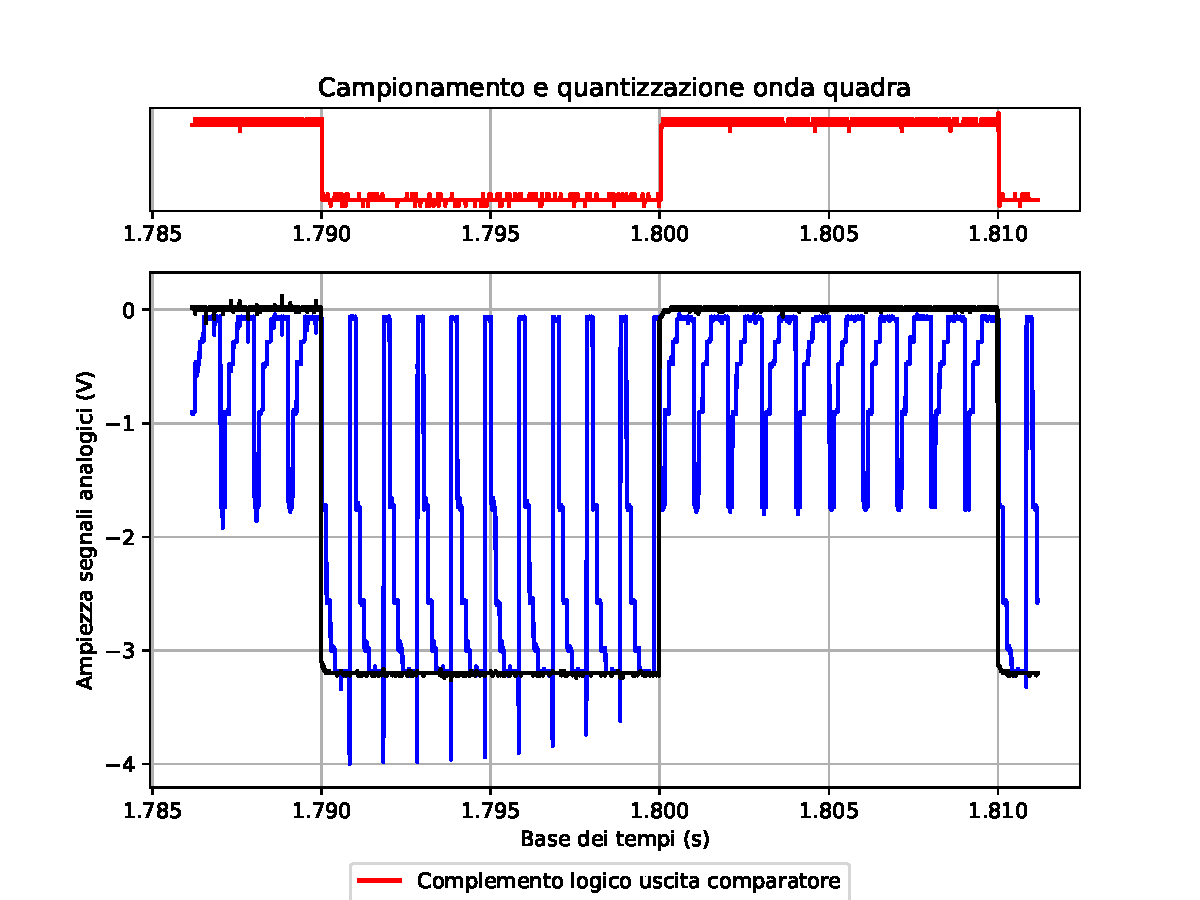
\includegraphics[trim = {0 25 0 0},clip, width=0.50\textwidth]{analysis/output/square_wave_aq.pdf}}
\caption{Didascalia}
\label{fig:circuit_DAC}
\end{center}
\end{figure}

\begin{figure*}[t]%[t]
\centering
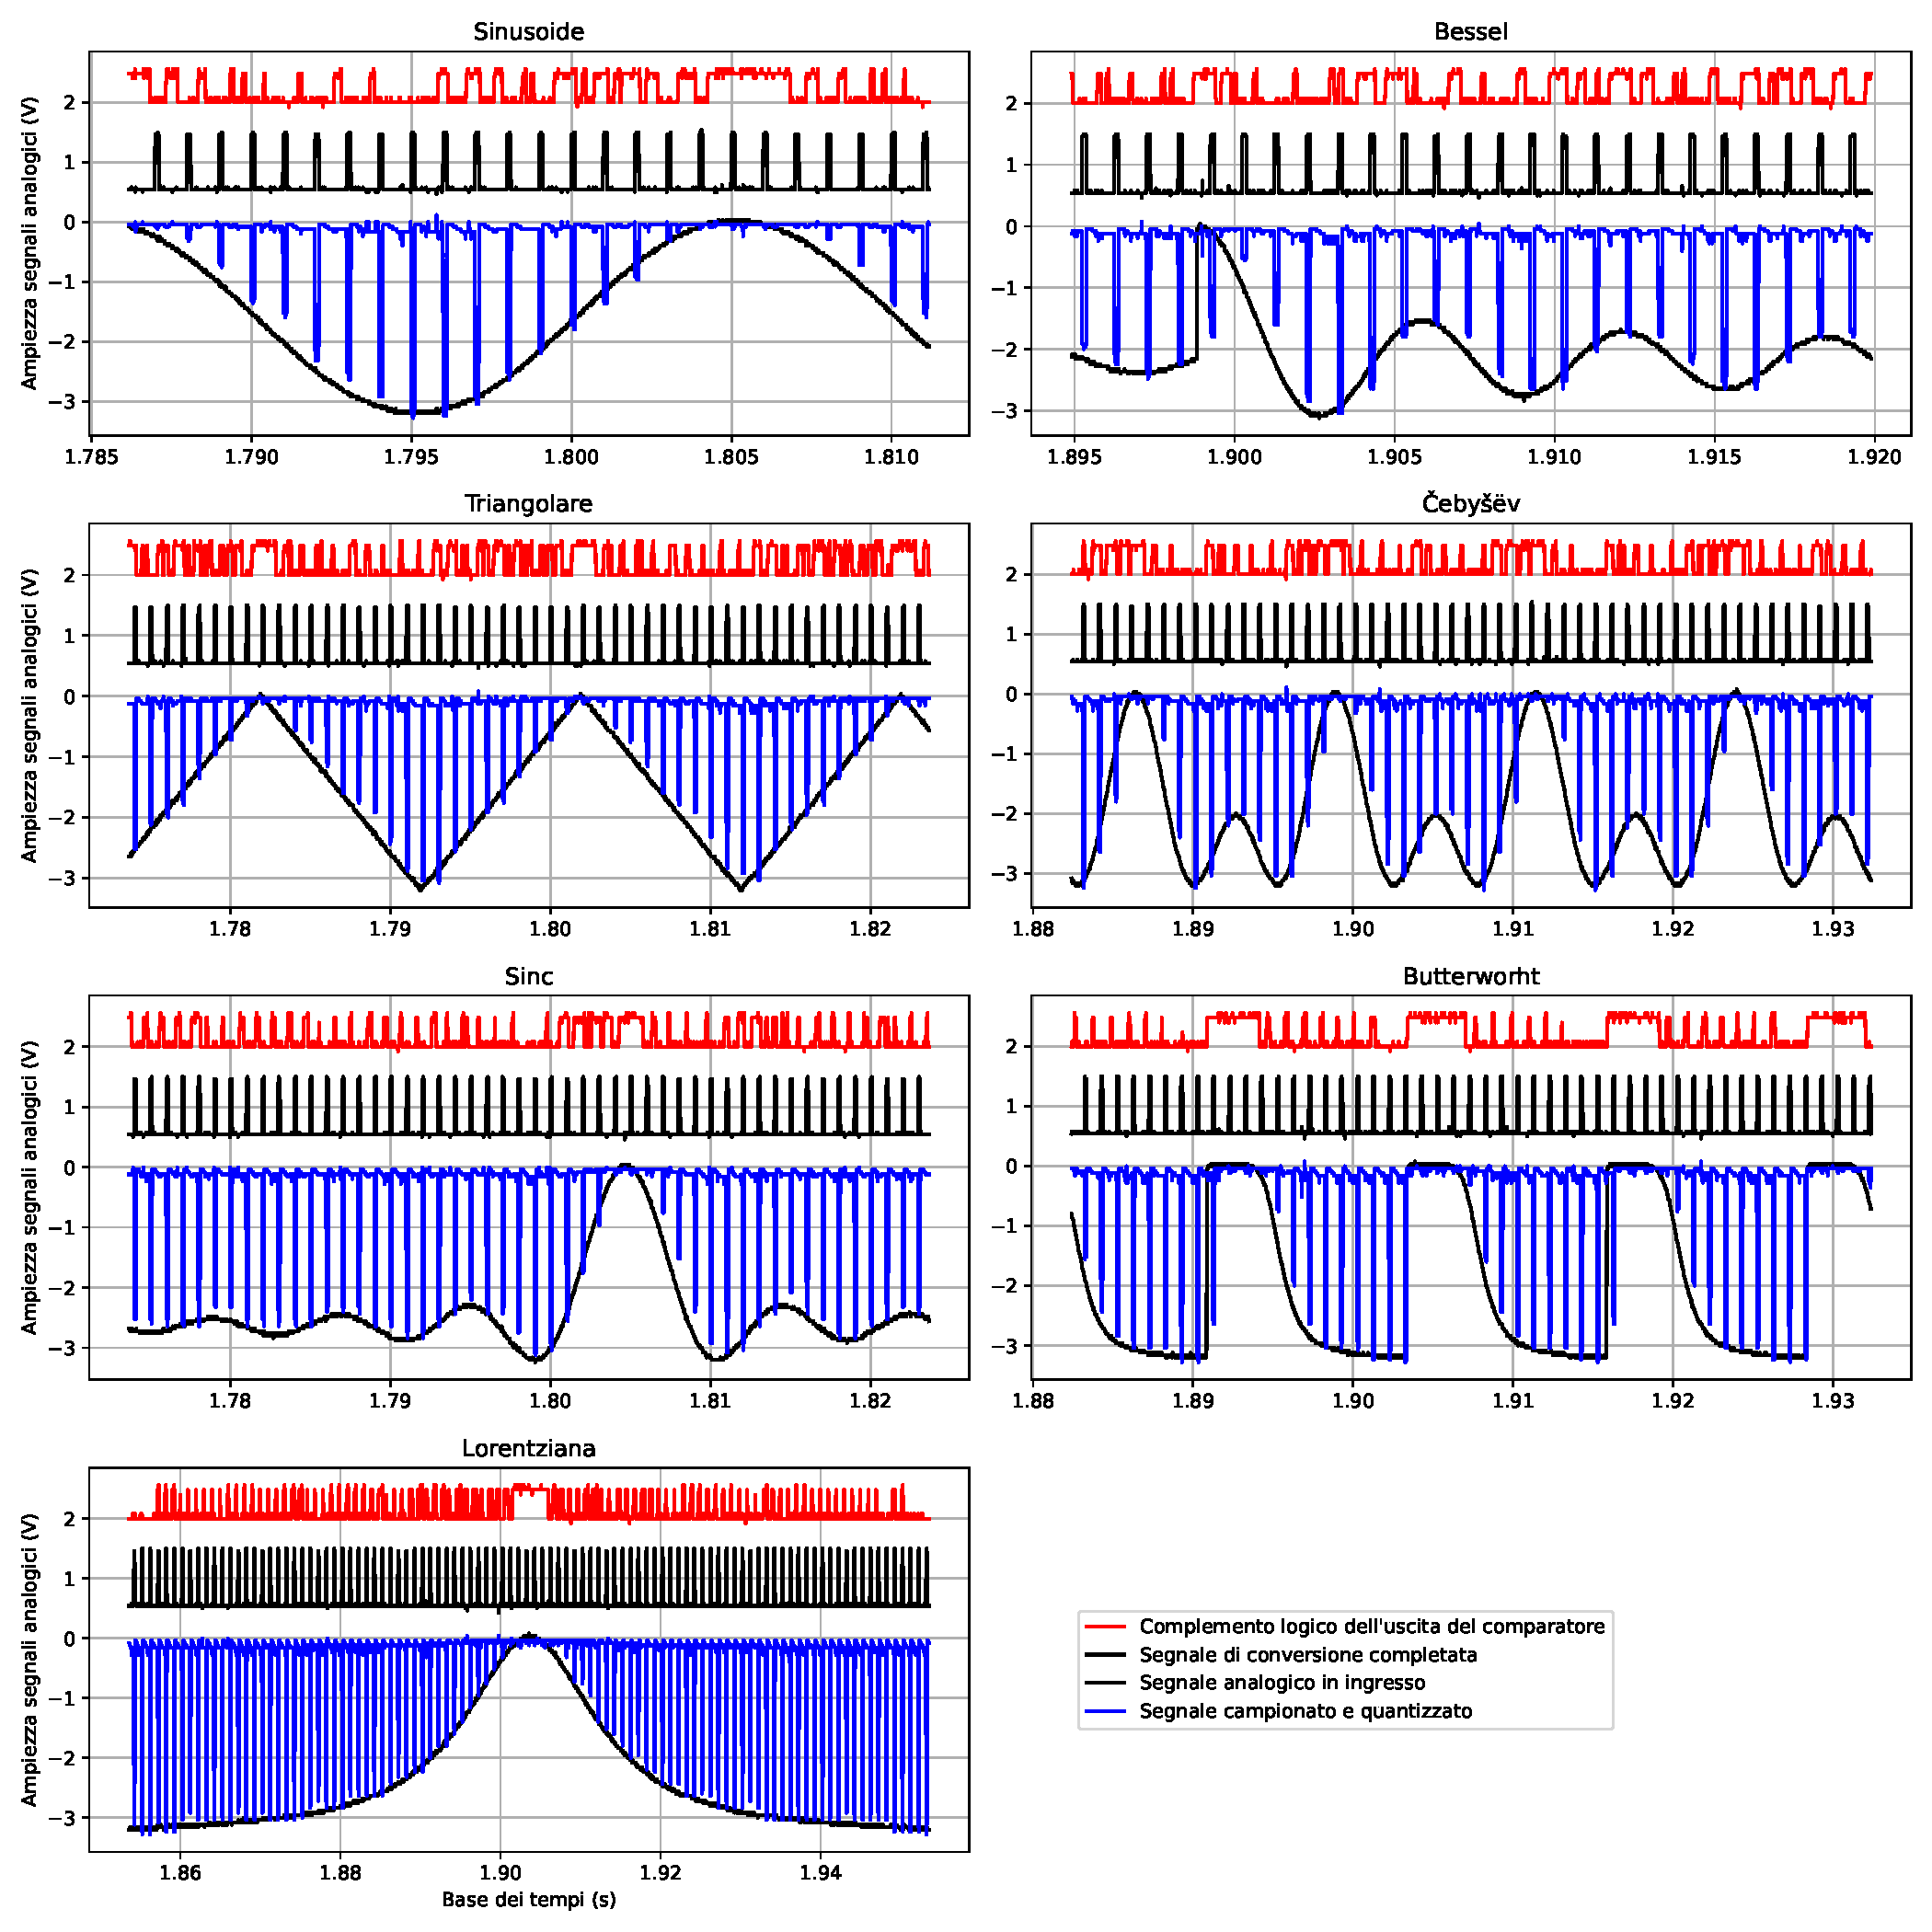
\includegraphics[trim = {30 0 50 0}, width=0.95\textwidth]{analysis/output/waveforms.pdf}
\caption{Schema elettrico completo del convertitore ADC SAR 4 bit}
\label{fig:waveforms_no_sh_scope}
\end{figure*}



\subsection{Circuito \textit{sample-hold}}
Testo


\begin{figure}[H]%[!ht]
\begin{center}
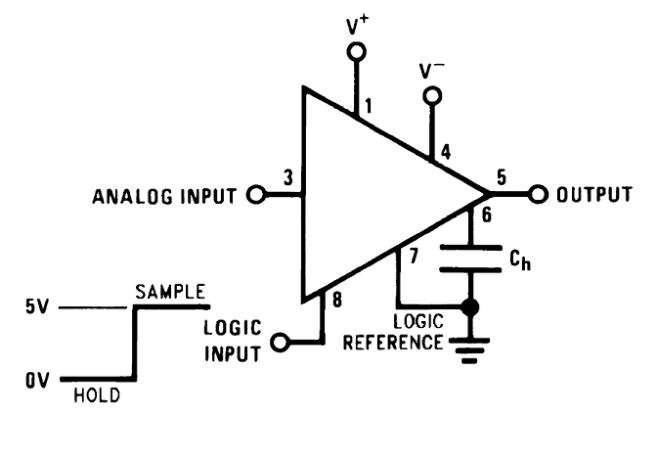
\includegraphics[width=0.35\textwidth]{sch-simulations/digital/output/lf398.png}
\caption{Schema di collegamento dell'integrato LF398 utilizzato in laboratorio per realizzare il circuito di \textit{sample and hold}, proveniente dal datasheet Texas Instruments del componente. Il valore del condensatore è $C_h$ = (0.00 $\pm$ 0.00) pF}
\label{fig:circuit_sample_and_hold}
\end{center}
\end{figure}

%%%%%%%%%%%%%%%%%%%%%%%%%%%%%%%%%%%%%%%%%%%%%%%%%%%%%%%%%%%%%
\section{Registrazione della conversione mediante scheda a microcontrollore}
Testo

\subsection{Verifica del teorema del campionamento di Nyquist-Shannon con sample-hold e oscilloscopio}
Testo

\clearpage
\clearpage
\begin{figure}[H]%[!ht]
\begin{center}
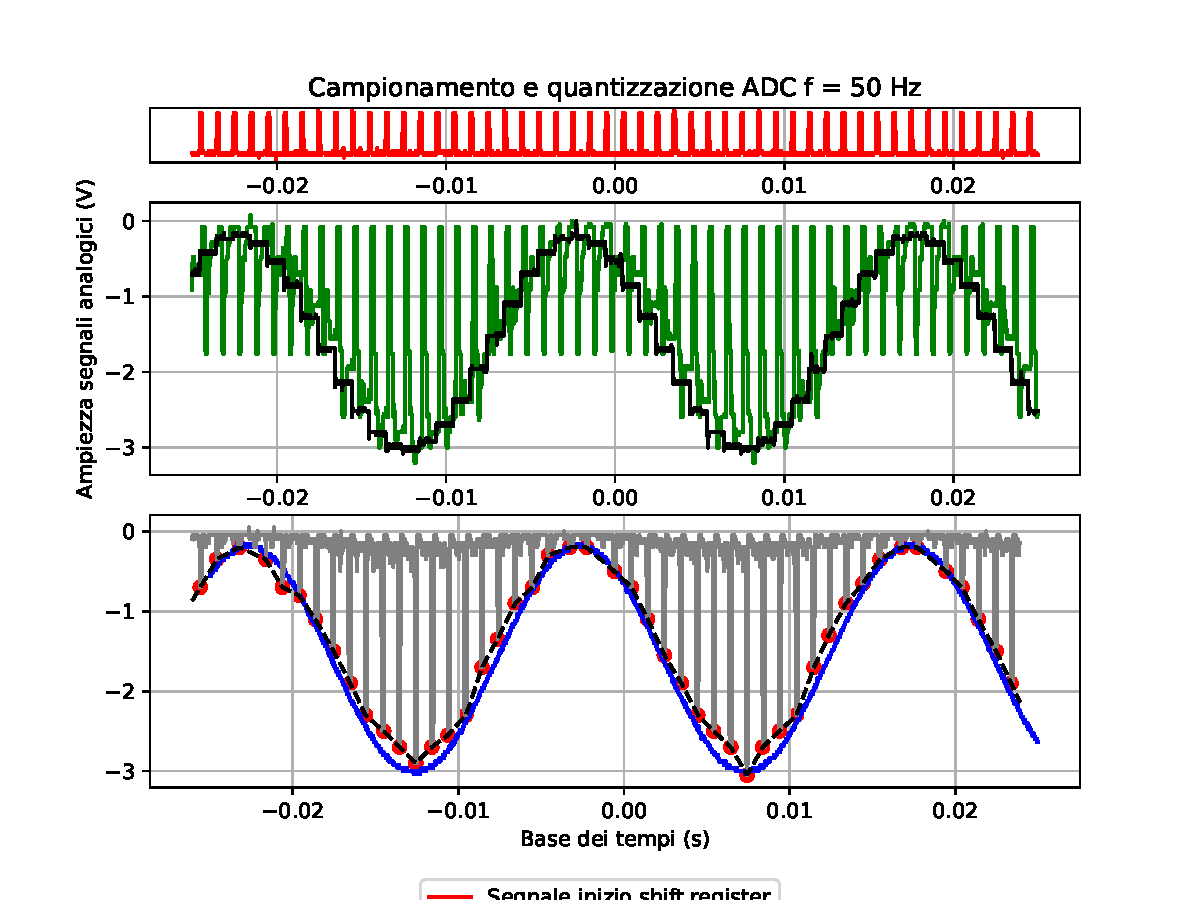
\includegraphics[trim={0 25 0 0}, clip, width=0.50\textwidth]{analysis/output/campionamento_50Hz.pdf}

\caption{Campionamento di forma d'onda sinusoidale f = 50 Hz. In rosso il segnale logico di controllo del sample-hold, in nero il segnale in uscita dal sample-hold, in verde il segnale in uscita dal DAC, il blu il segnale analogico in ingresso e in grigio il segnale ricostruito dall'ADC.}
\label{fig:graph_ring_oscillator}
\end{center}
\end{figure}
\vspace{-10mm}
%
\begin{figure}[H]%[!ht]
\begin{center}
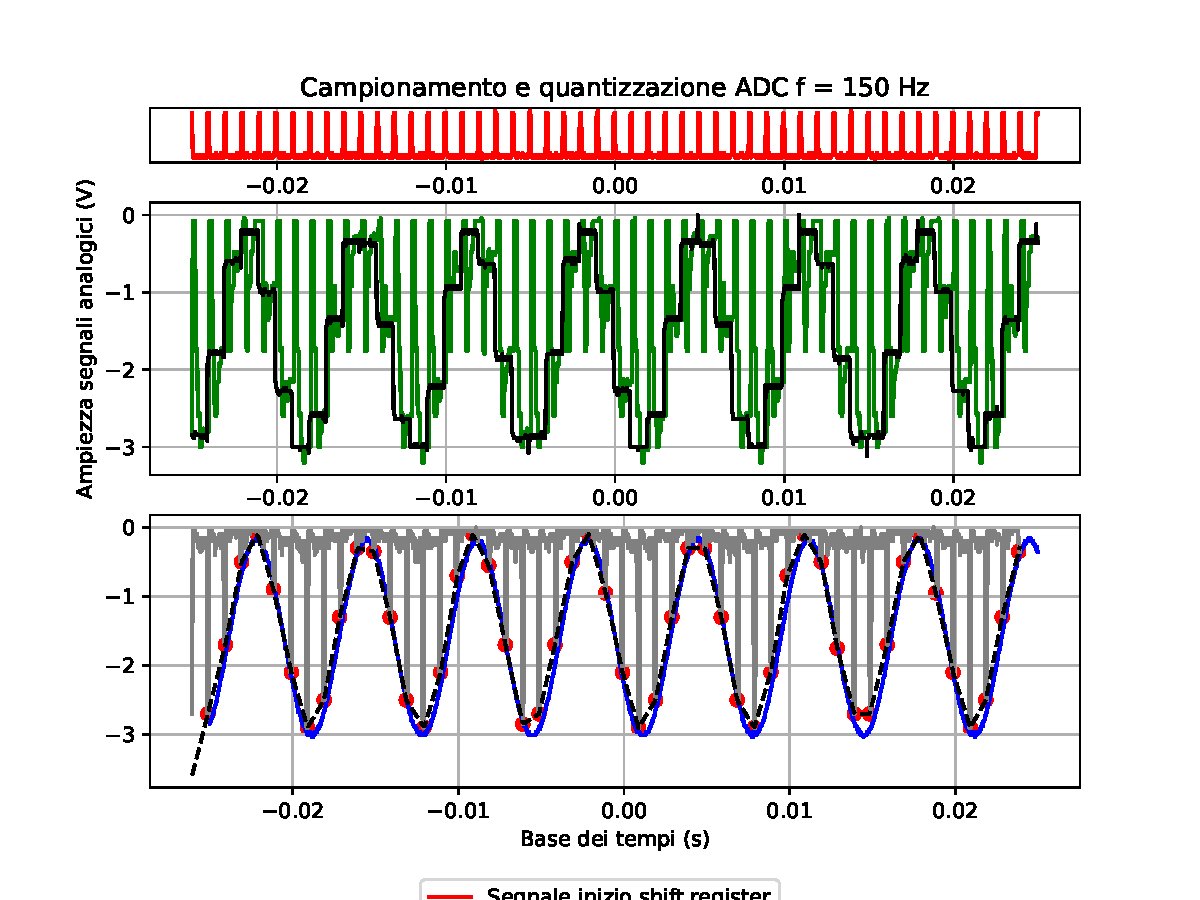
\includegraphics[trim={0 25 0 0}, clip,width=0.50\textwidth]{analysis/output/campionamento_150Hz.pdf}
\caption{Campionamento di forma d'onda sinusoidale f = 150 Hz, colori come nella figura precedente.}
\label{fig:graph_ring_oscillator}
\end{center}
\end{figure}
\vspace{-10mm}
%
\begin{figure}[H]%[!ht]
\begin{center}
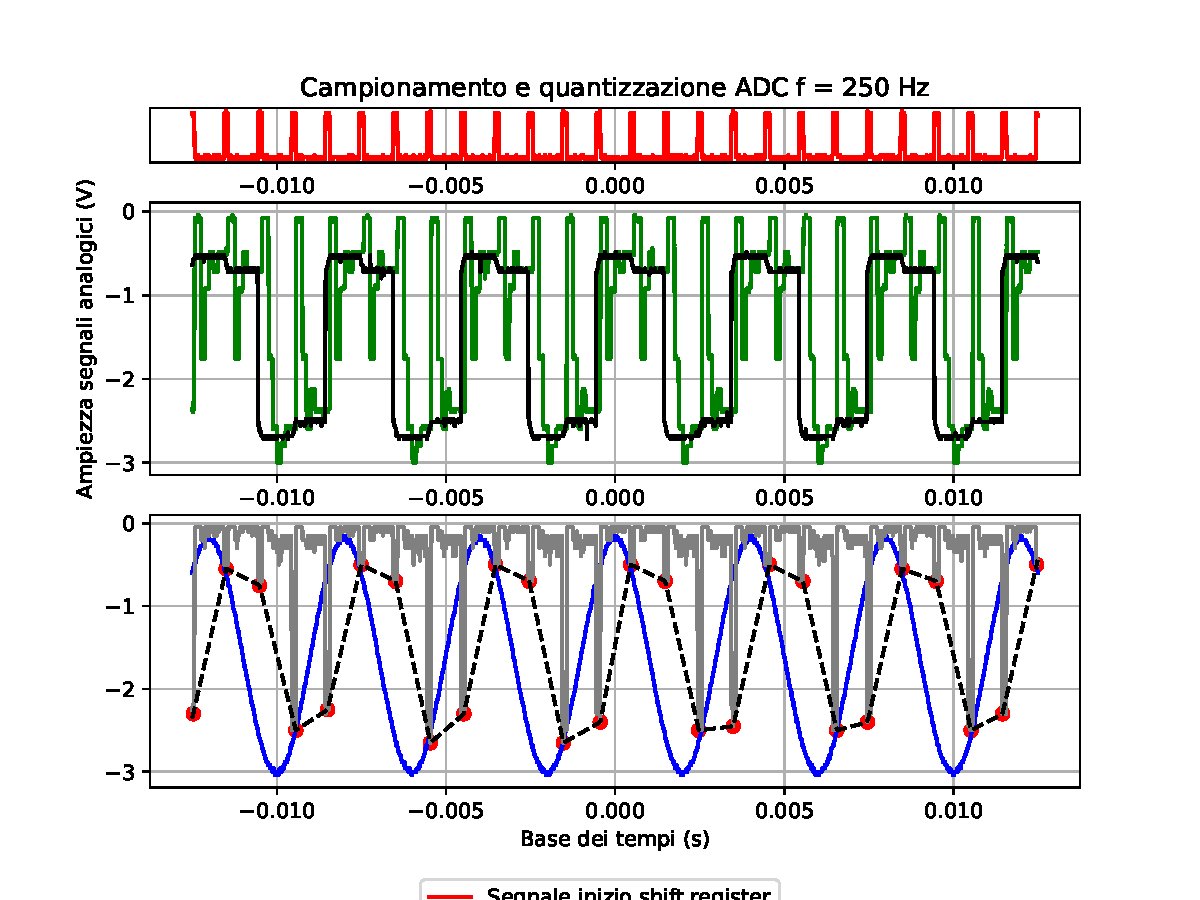
\includegraphics[trim={0 25 0 0}, clip,width=0.50\textwidth]{analysis/output/campionamento_250Hz.pdf}
\caption{Campionamento di forma d'onda sinusoidale f = 250 Hz, colori come nella figura precedente.}
\label{fig:graph_ring_oscillator}
\end{center}
\end{figure}
\vspace{-10mm}
%
\begin{figure}[H]%[!ht]
\begin{center}
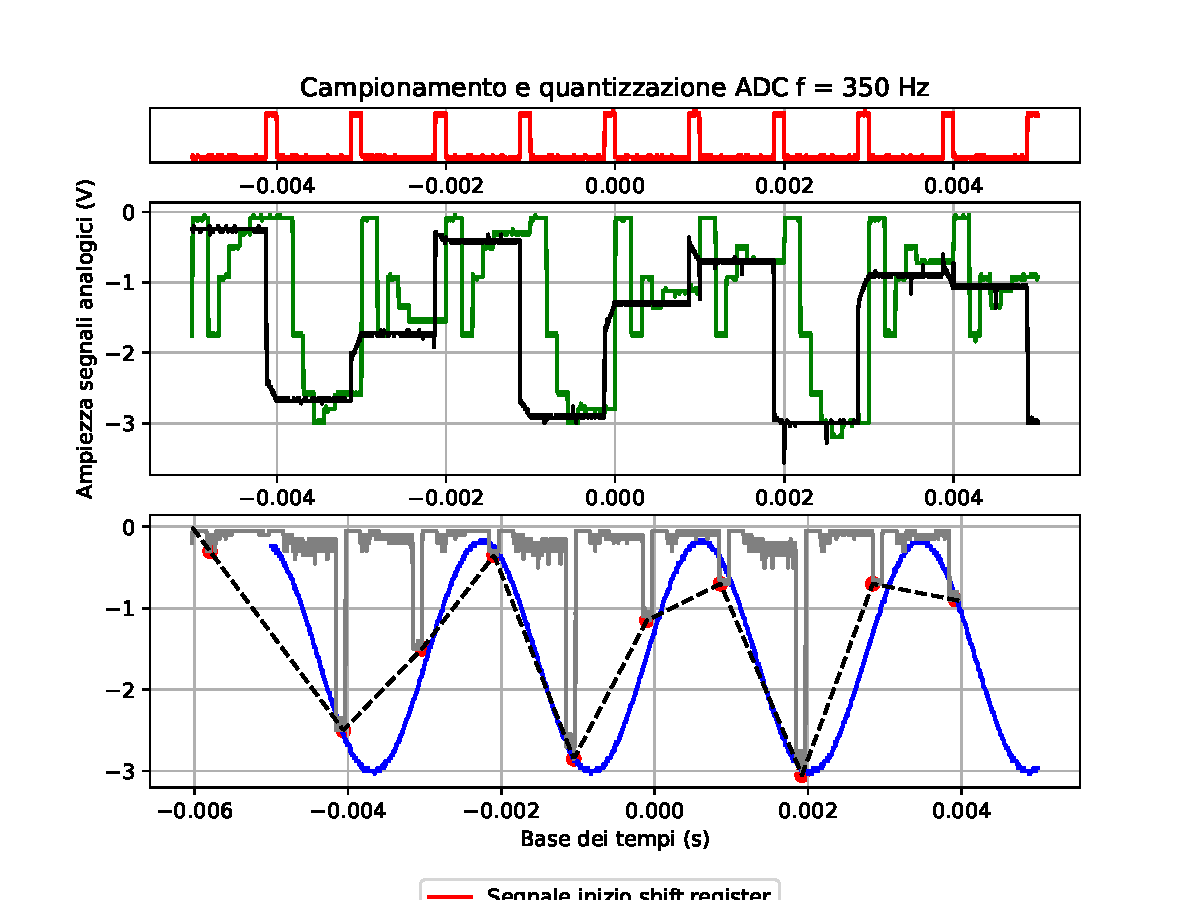
\includegraphics[trim={0 40 0 0}, clip,width=0.50\textwidth]{analysis/output/campionamento_350Hz.pdf}
\caption{Campionamento di forma d'onda sinusoidale f = 350 Hz, colori come nella figura precedente.}
\label{fig:graph_ring_oscillator}
\end{center}
\end{figure}
\vspace{-10mm}
%
\begin{figure}[H]%[!ht]
\begin{center}
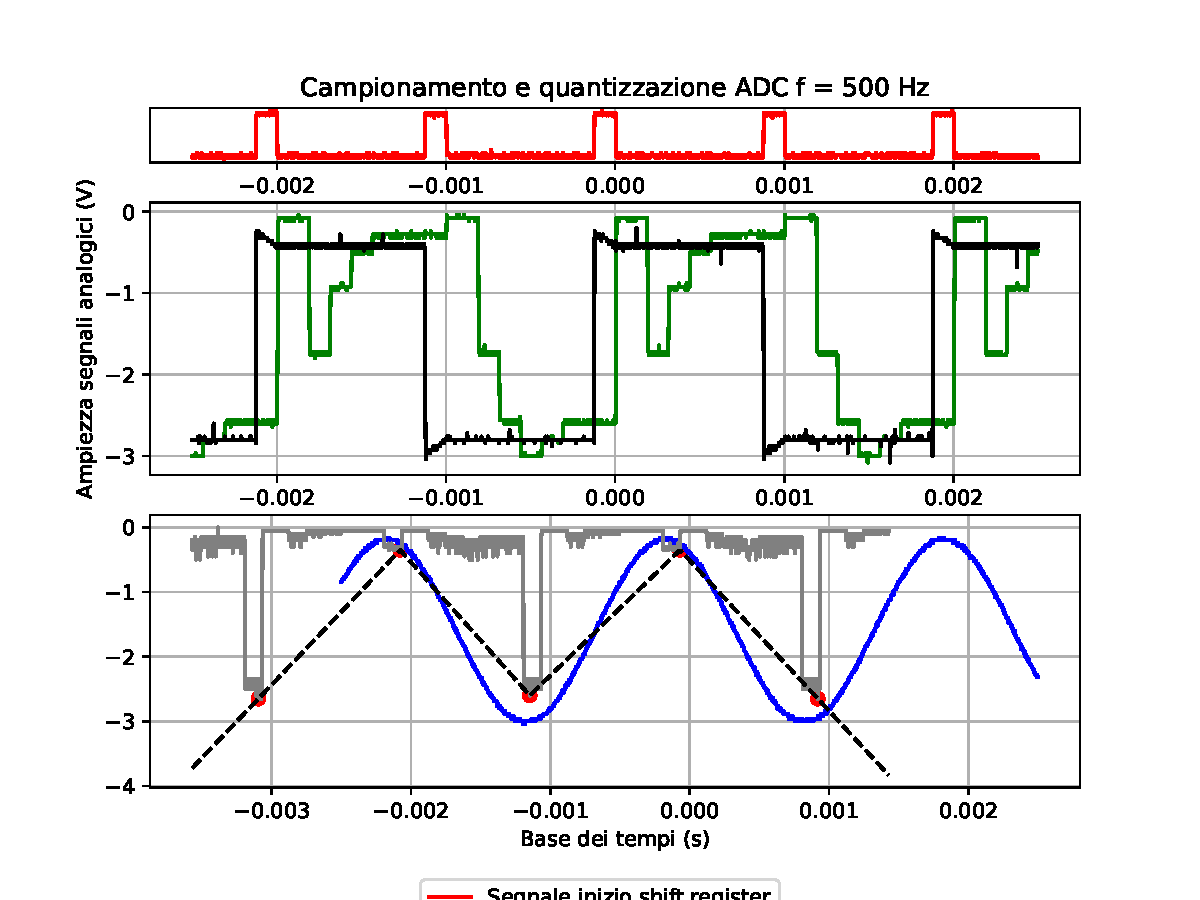
\includegraphics[trim={0 40 0 0}, clip,width=0.50\textwidth]{analysis/output/campionamento_500Hz.pdf}
\caption{Campionamento di forma d'onda sinusoidale f = 500 Hz, colori come nella figura precedente.}
\label{fig:graph_ring_oscillator}
\end{center}
\end{figure}
\vspace{-10mm}
%
\begin{figure}[H]%[!ht]
\begin{center}
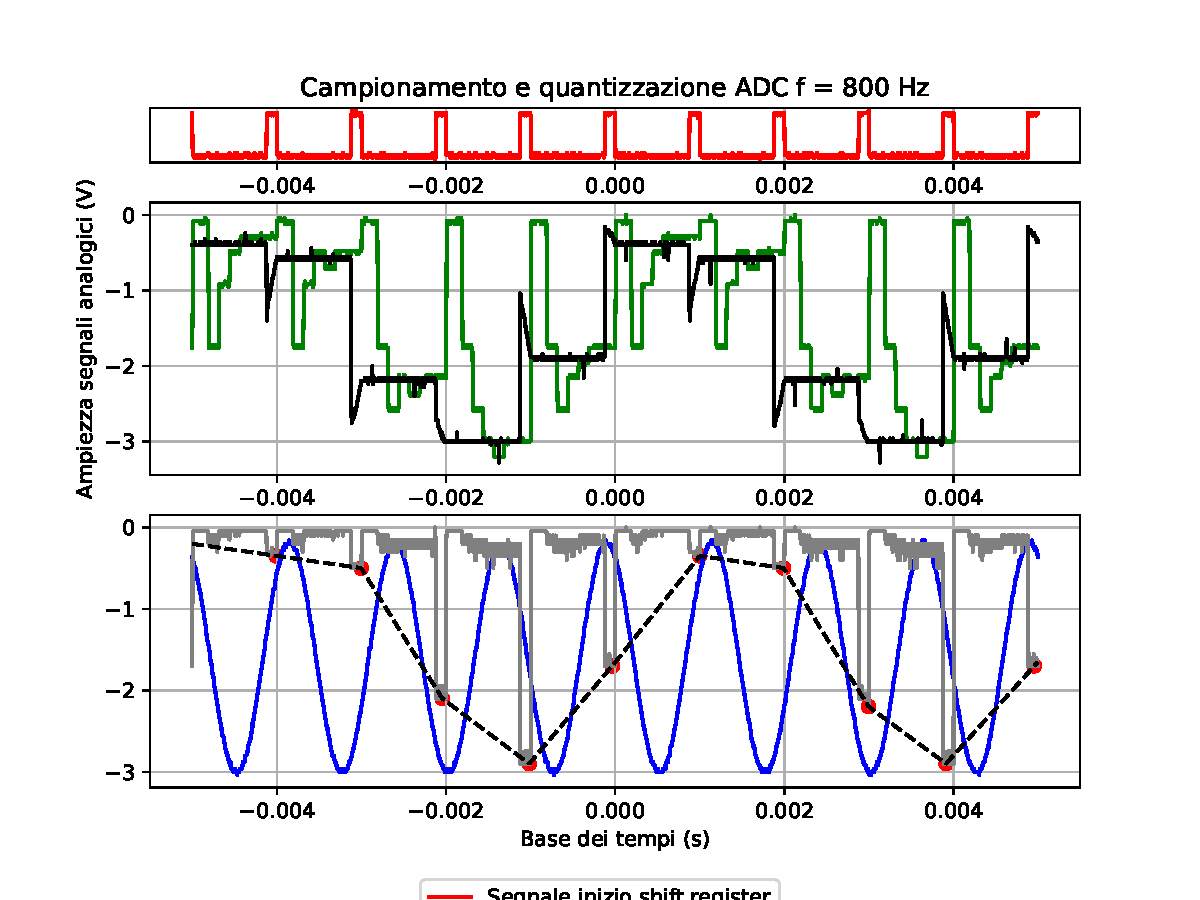
\includegraphics[trim={0 40 0 0}, clip,width=0.50\textwidth]{analysis/output/campionamento_800Hz.pdf}
\caption{Campionamento di forma d'onda sinusoidale f = 800 Hz, colori come nella figura precedente.}
\label{fig:graph_ring_oscillator}
\end{center}
\end{figure}

\subsection{Verifica del teorema del campionamento di Nyquist-Shannon con sample-hold e acquisizione con microcontrollore}

\begin{figure}[H]%[!ht]
\begin{center}
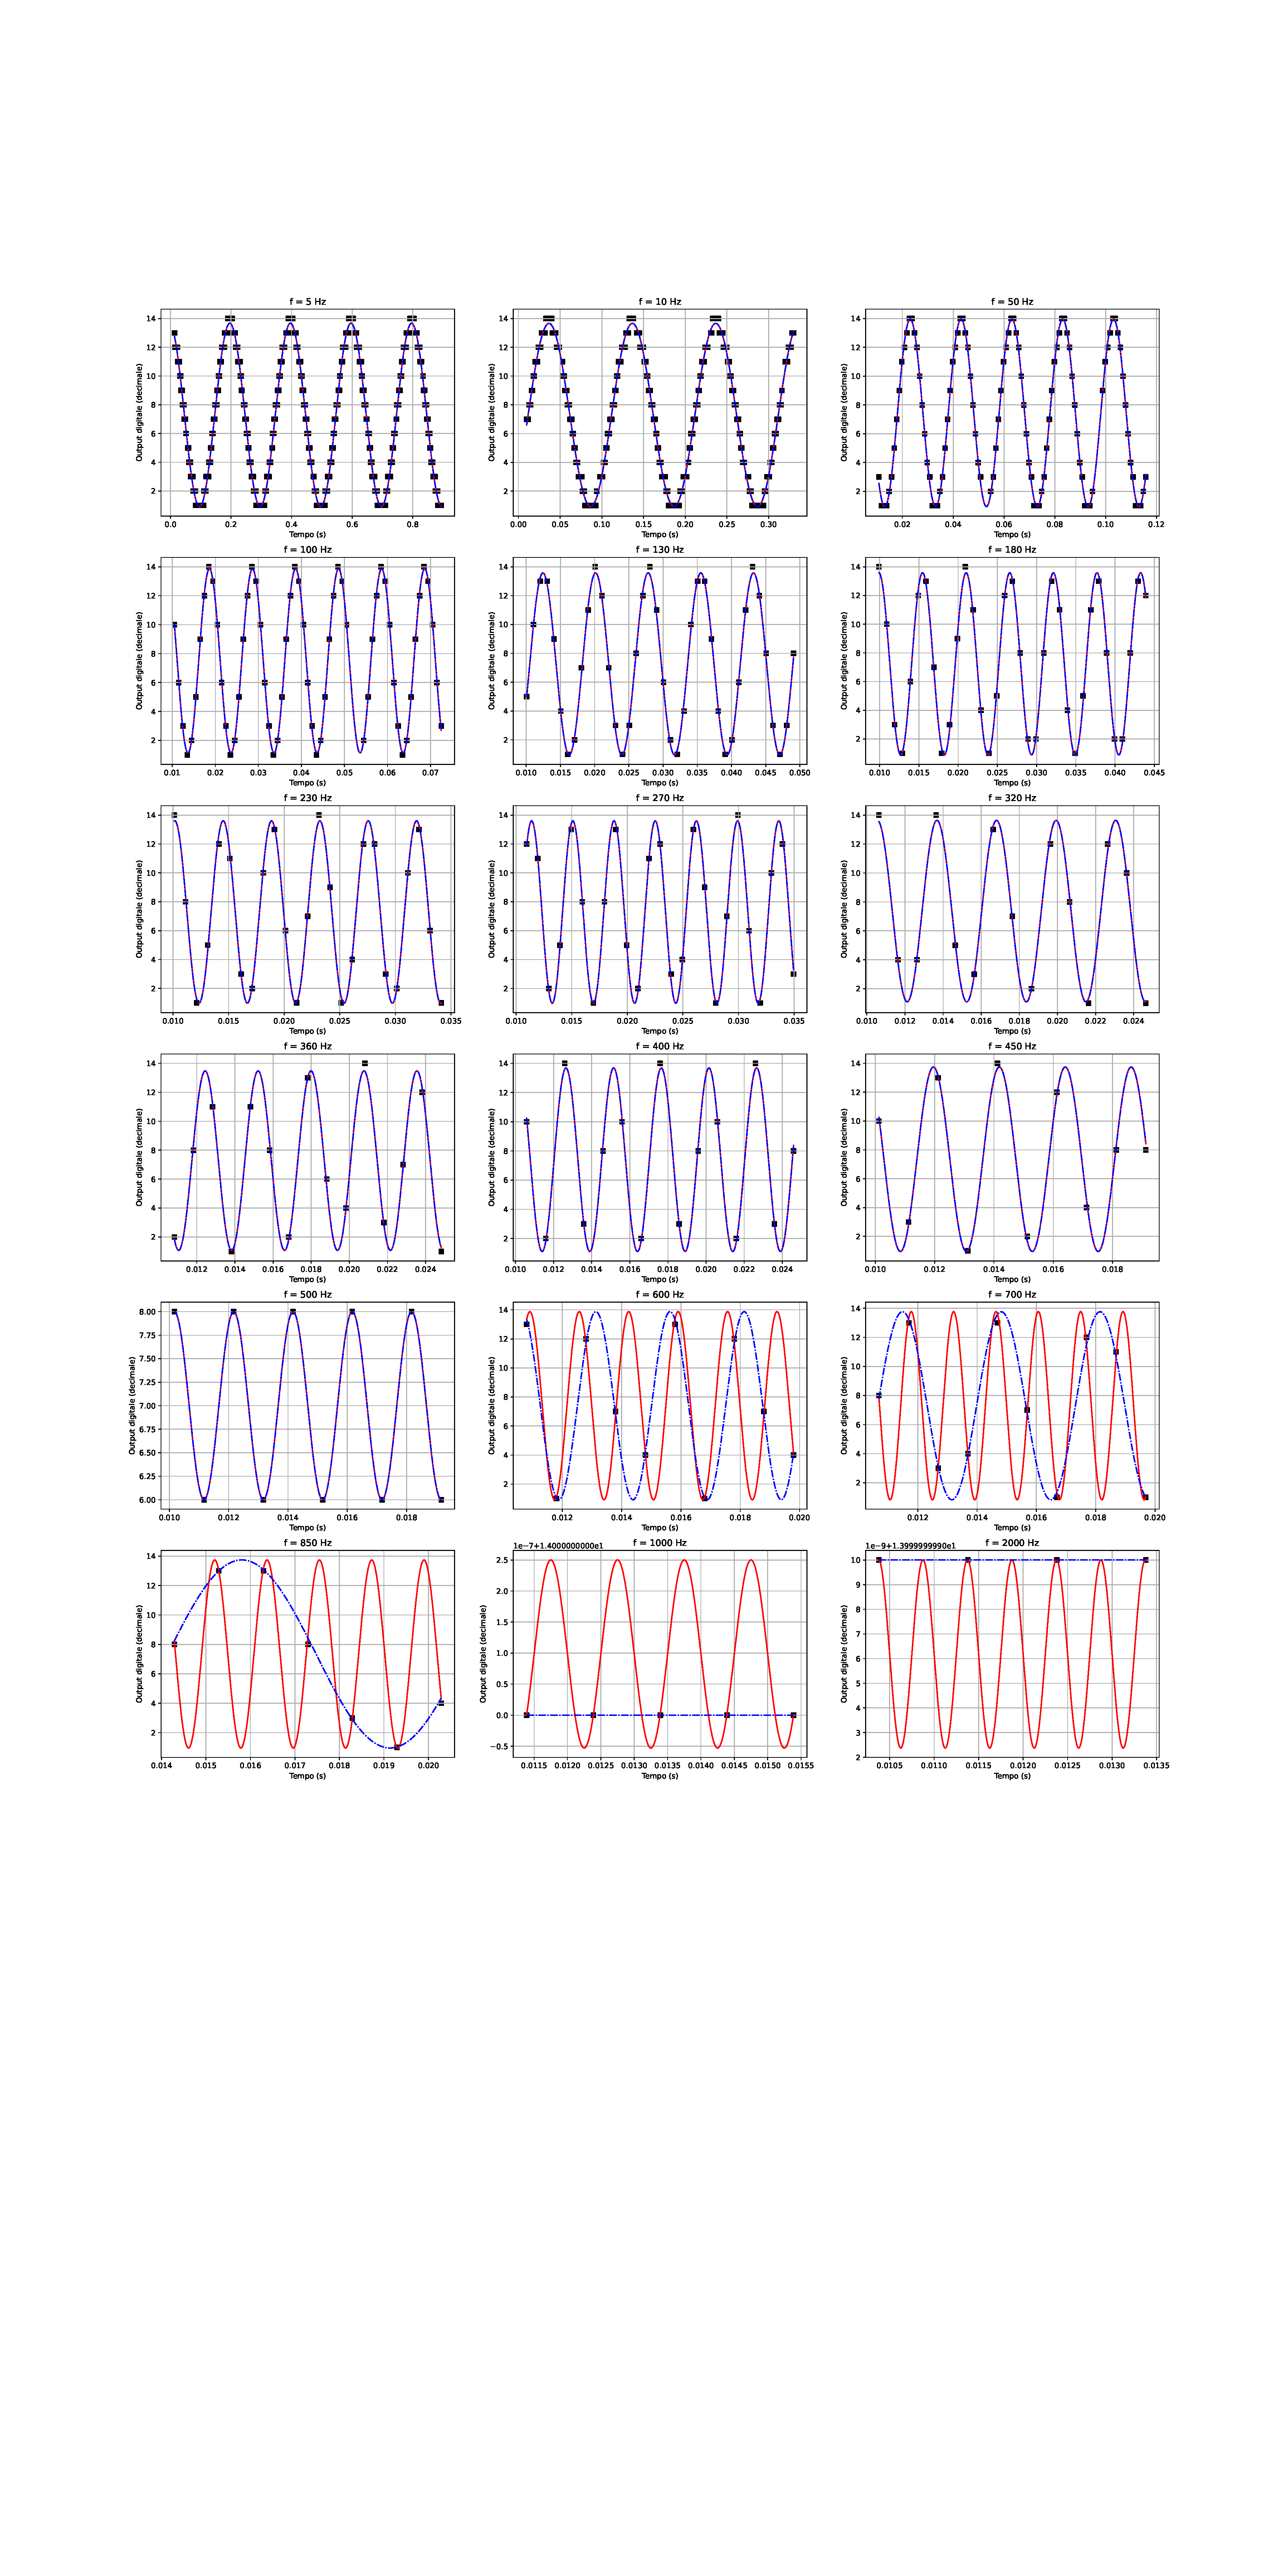
\includegraphics[width=0.48\textwidth]{analysis/output/cumulative_nyquist_mcu.pdf}
\caption{campionamento di segnale sinusoidale con frequenze da 5 a 2000 Hz}
\label{fig:nyquist_mcu_cumulative}
\end{center}
\end{figure}




\subsection{Valutazione della linearità con metodo della \textit{code density}}

\begin{figure}[H]%[!ht]
\begin{center}
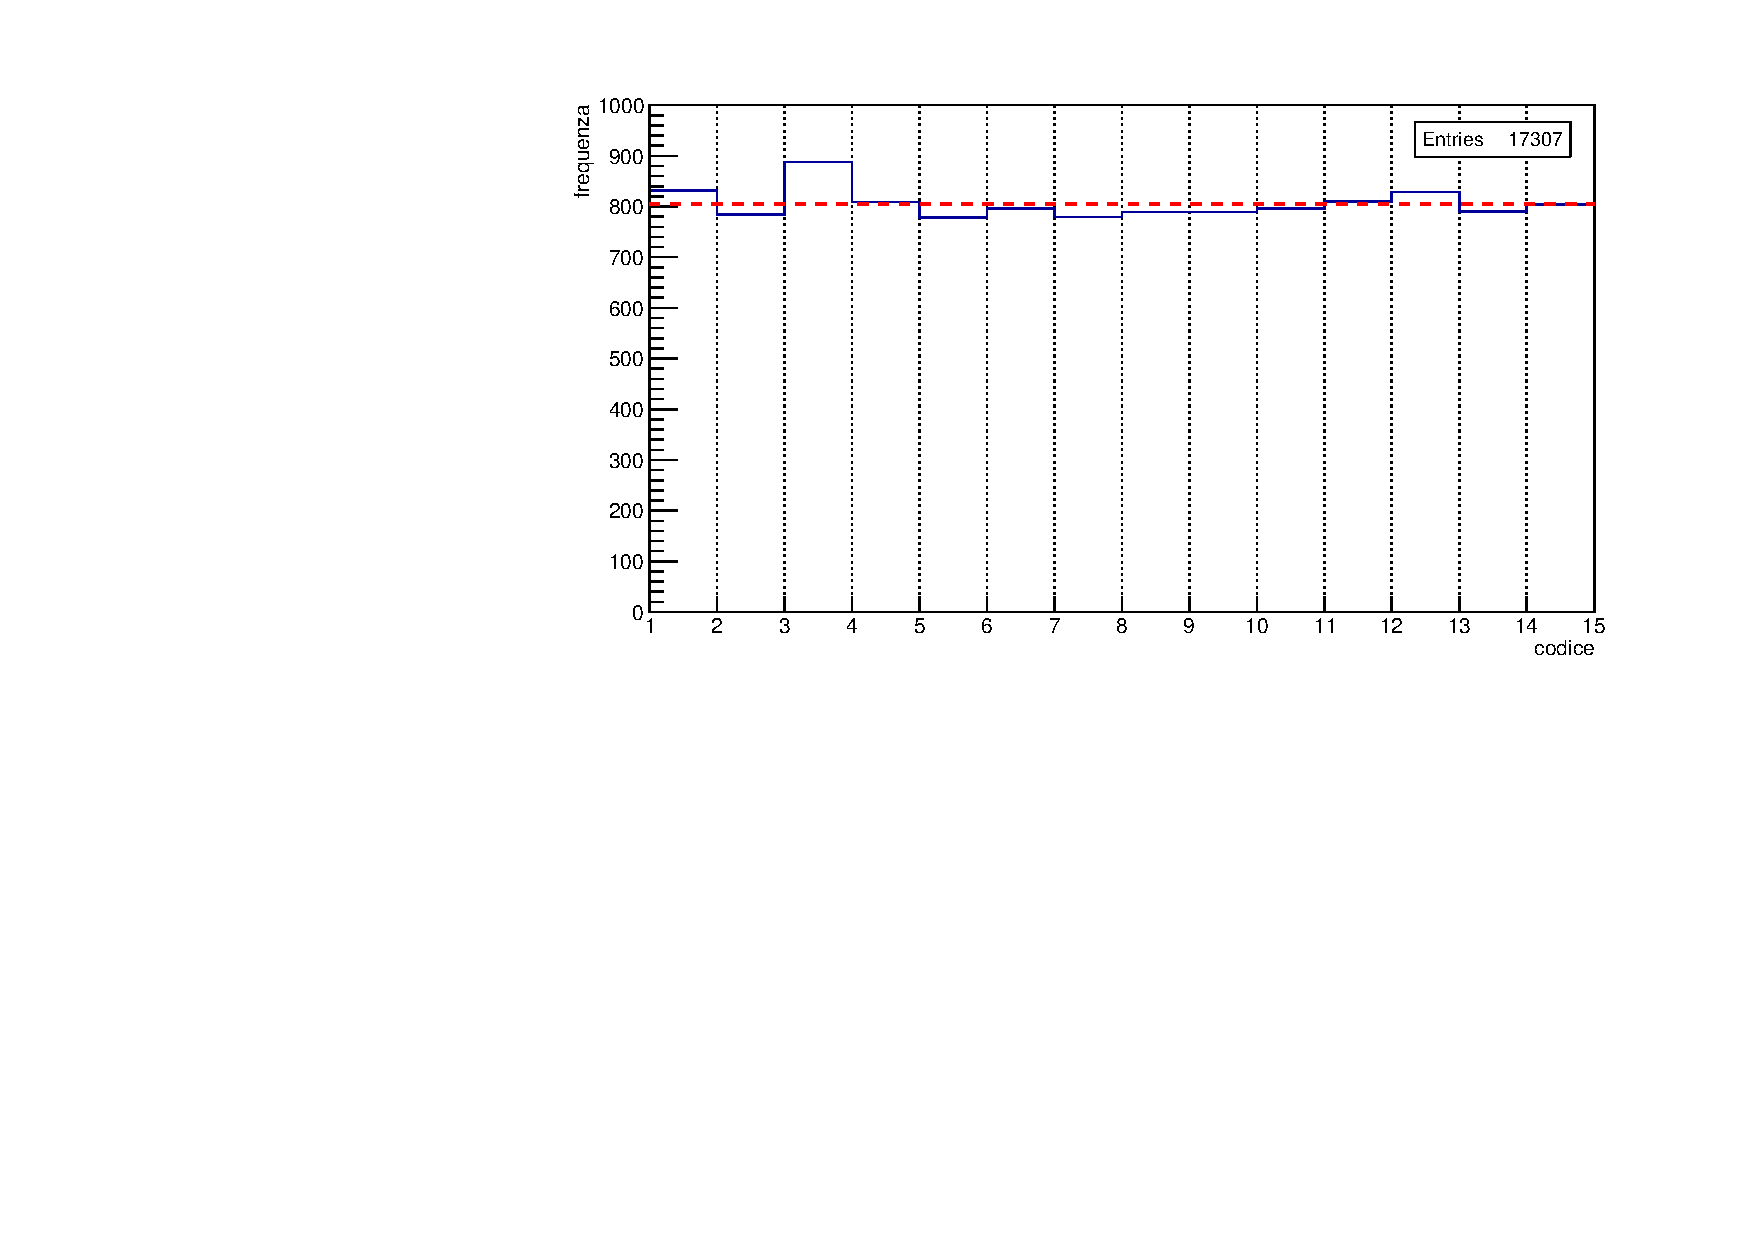
\includegraphics[width=0.48\textwidth]{analysis/output/dnl_800_hz.pdf}
\caption{Istogramma delle frequenze di occupazione dei codici: frequenza di clock pari a 800 Hz}
\label{fig:graph_dnl_800_hz}
\end{center}
\end{figure}



\begin{figure}[H]%[!ht]
\begin{center}
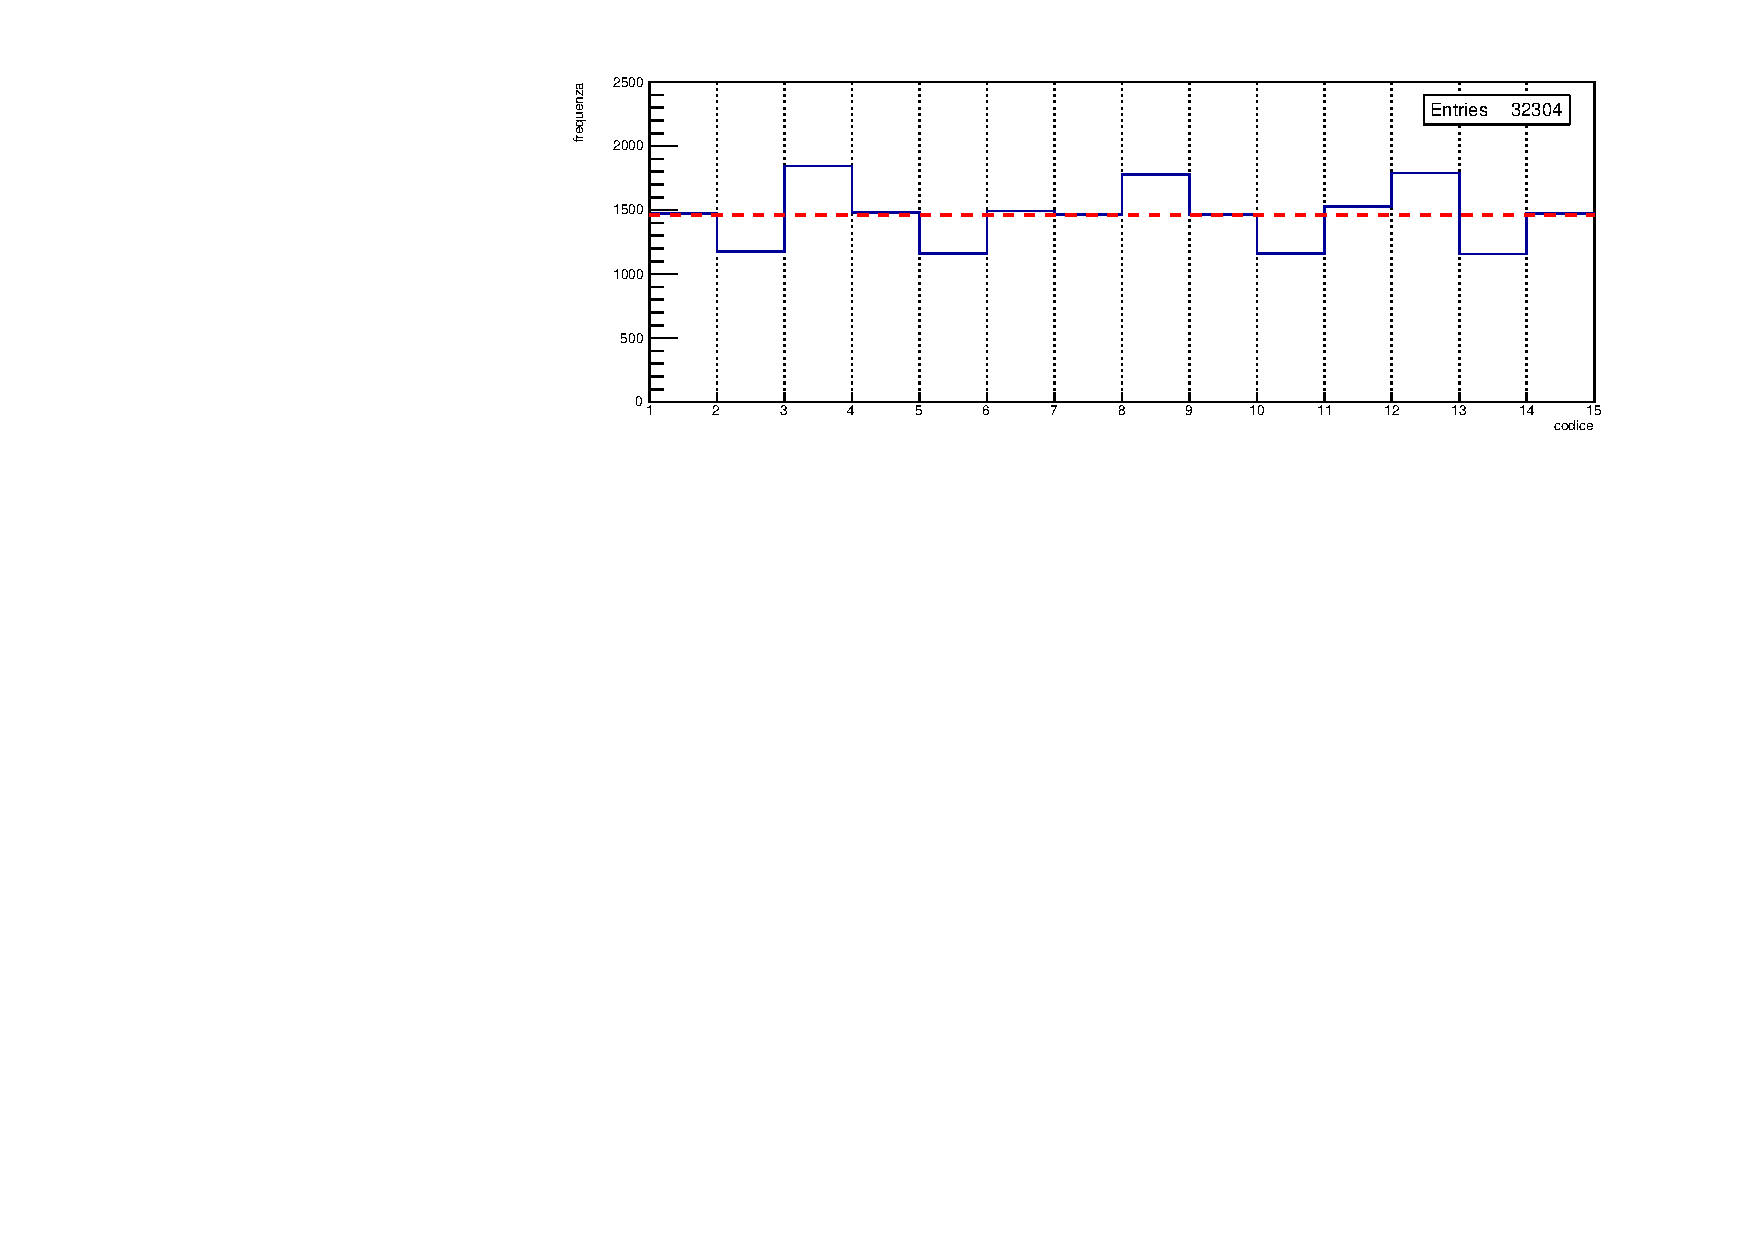
\includegraphics[width=0.48\textwidth]{analysis/output/dnl_8000_hz_S28.pdf}
\caption{Istogramma delle frequenze di occupazione dei codici: frequenza di clock pari a 8000 Hz}
\label{fig:graph_dnl_8000_hz_S28}
\end{center}
\end{figure}


%%%%%%%%%%%%%%%%%%%%%%%%%%%%%%%%%%%%%%%%%%%%%%%%%%%%%%%%%%%%%
\section{Discussione dei risultati e conclusioni}
Testo


\begin{figure*}[t]%[t]
\centering
\begin{center}
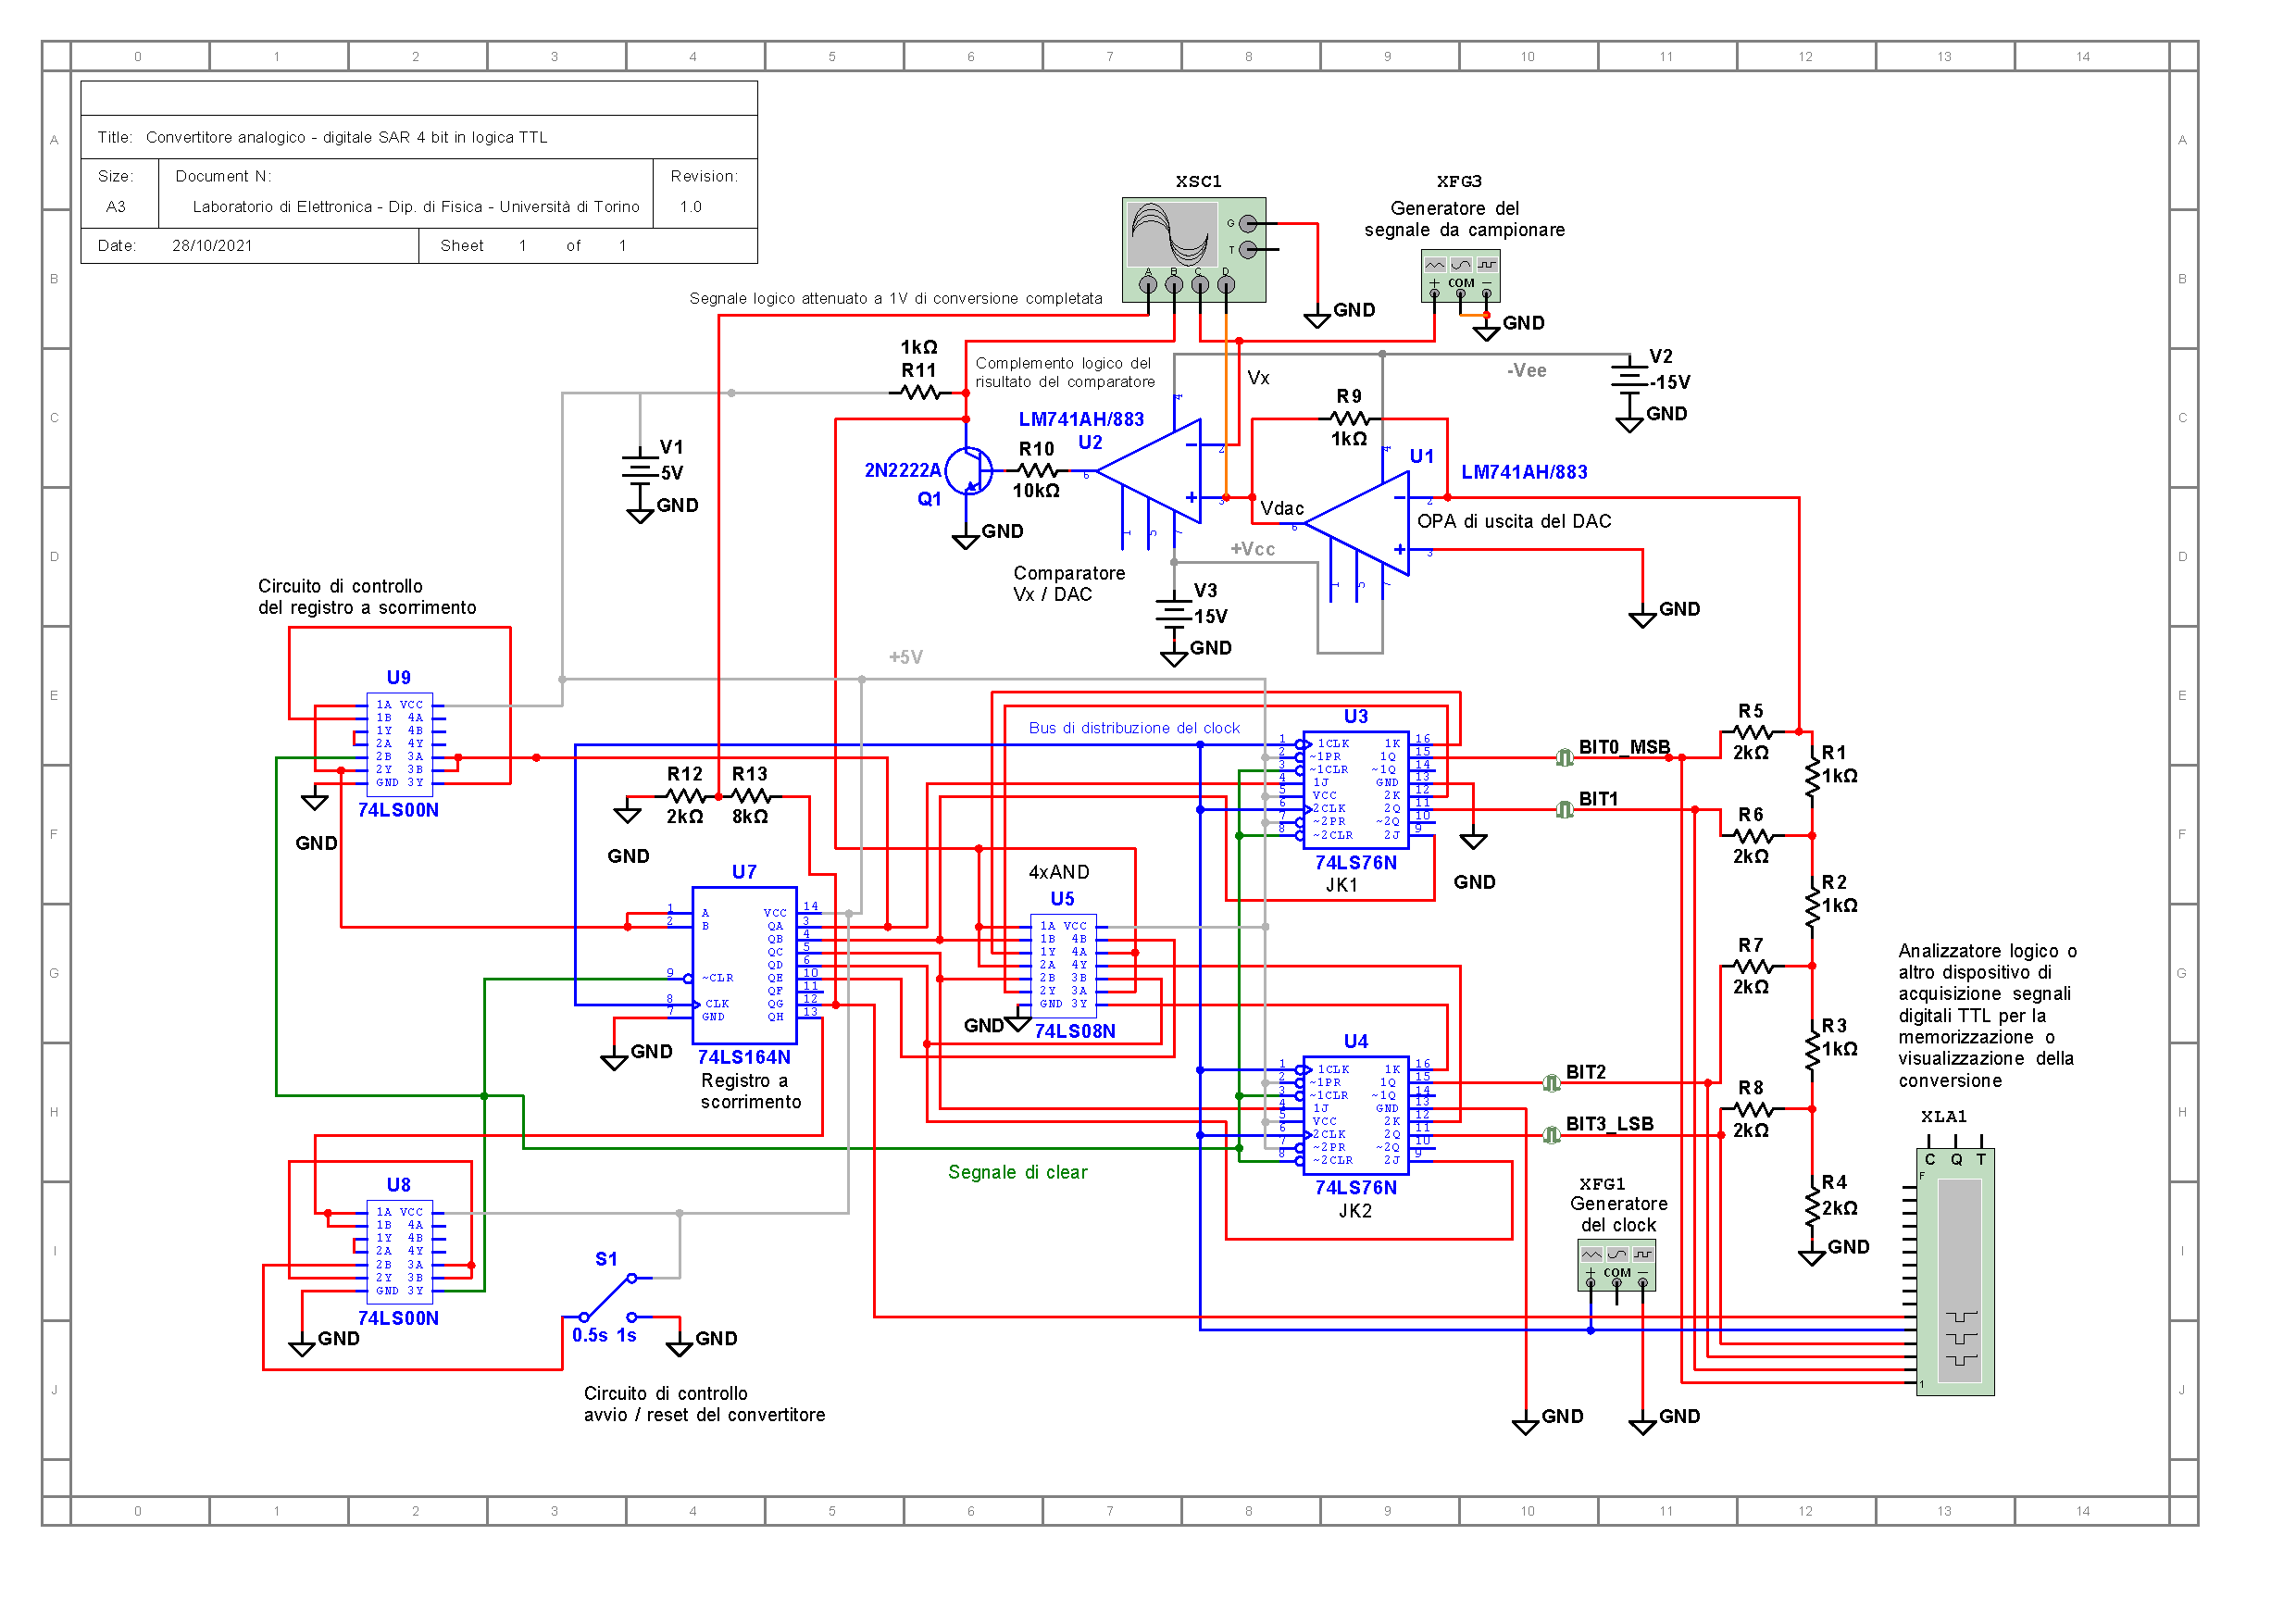
\includegraphics[trim = {0 0 50 0}, width=1.40\textwidth, angle=90]{sch-simulations/digital/output/Schema_convertitore_completo.pdf}
\end{center}
\caption{Schema elettrico completo del convertitore ADC SAR 4 bit}
\label{fig:circuit_sarCompleteSchematic}
\end{figure*}



%%%%%%%%%%%%%%%%%%%%%%%%%%%%%%%%%%%%%%%%%%%%%%%%%%%%%%%%%%%%%
%% Appendice
%%%%%%%%%%%%%%%%%%%%%%%%%%%%%%%%%%%%%%%%%%%%%%%%%%%%%%%%%%%%%

\clearpage

\begin{appendices}

\section{Tabella calibrazione DAC}

\centering
\begin{tabular}{cc}
binario & V $ \pm 0.1 \ V $ \\ \hline
0       & 0.0                          \\
1       & -0.3                       \\
10      & -0.6                       \\
11      & -0.9                       \\
100     & -1.2                       \\
101     & -1.6                       \\
110     & -1.9                       \\
111     & -2.2                       \\
1000    & -2.5                       \\
1001    & -2.8                       \\
1010    & -3.1                       \\
1011    & -3.4                       \\
1100    & -3.7                       \\
1101    & -4.0                       \\
1110    & -4.3                       \\
1111    & -4.6
\vspace{5 mm}
%\caption{}
\label{tab:calibrazione_dac}
\end{tabular}


\section{Tabella calibrazione ADC}

\begin{tabular}{cc}
binario & $V_{min}  \pm 0.1 \ V$ \\ \hline
1111    & -3.2                  \\
1110    & -3.0                  \\
1101    & -2.7                  \\
1100    & -2.5                  \\
1011    & -2.3                  \\
1010    & -2.1                  \\
1001    & -1.9                  \\
1000    & -1.7                  \\
111     & -1.5                  \\
110     & -1.3                  \\
101     & -1.0                  \\
100     & -0.8                  \\
11      & -0.7                  \\
10      & -0.5                  \\
1       & -0.2                  \\
0       & 0.0
\vspace{5 mm}
%\caption{}
\label{tab:calibrazione_adc}
\end{tabular}


\end{appendices}

%%%%%%%%%%%%%%%%%%%%%%%%%%%%%%%%%%%%%%%%%%%%%%%%%%%%%%%%%%%%%
%% Indice e Bibliografia 
%%%%%%%%%%%%%%%%%%%%%%%%%%%%%%%%%%%%%%%%%%%%%%%%%%%%%%%%%%%%%

\clearpage
\newpage

\tableofcontents % Indice

\newpage

\printbibliography % Bibliografia

\end{document}